\documentclass[aos]{imsart}

\RequirePackage{amsthm,amsmath,amsfonts,amssymb}
\RequirePackage[authoryear]{natbib}
\RequirePackage[colorlinks,citecolor=blue,urlcolor=blue]{hyperref}
\RequirePackage{graphicx}
\usepackage{booktabs}
\usepackage{nicefrac}
\usepackage{microtype}
\usepackage{xcolor}
\usepackage{comment}
\usepackage{multirow}
\usepackage{threeparttable}
\usepackage{algorithm}
\usepackage{algpseudocode}
\usepackage{grffile}
\usepackage{wrapfig}

\DeclareFontShape{T1}{ptm}{m}{scit}{<->ssub*ptm/m/sc}{}

\startlocaldefs
\numberwithin{equation}{section}

\theoremstyle{plain}
\newtheorem{theorem}{Theorem}[section]
\newtheorem{lemma}[theorem]{Lemma}
\newtheorem{corollary}[theorem]{Corollary}
\newtheorem{proposition}[theorem]{Proposition}
\newtheorem{claim}[theorem]{Claim}
\newtheorem{conjecture}[theorem]{Conjecture}
\newtheorem{fact}[theorem]{Fact}

\theoremstyle{definition}
\newtheorem{definition}[theorem]{Definition}
\newtheorem{assumption}[theorem]{Assumption}
\newtheorem{example}[theorem]{Example}
\newtheorem{observation}[theorem]{Observation}
\newtheorem{problem}[theorem]{Problem}

\theoremstyle{definition}
\newtheorem{remark}[theorem]{Remark}

\newcommand{\poly}{\mathrm{poly}}
\newcommand{\polylog}{\mathrm{polylog}}

\newcommand{\vecz}{\mathrm{vec}} % vectorize

\newcommand{\diag}{\mathrm{diag}}
\newcommand{\rank}{\mathrm{rank}}
\newcommand{\fed}{\mathrm{fed}}
\newcommand{\var}{\mathrm{Var}}
\newcommand{\cov}{\mathrm{Cov}}
\newcommand{\acc}{\mathrm{acc}}
\newcommand{\test}{\mathrm{test}}
\newcommand{\train}{\mathrm{train}}
\newcommand{\tr}{\mathrm{tr}}
\newcommand{\KL}{\mathrm{KL}}
\newcommand{\TV}{\mathrm{TV}}
\newcommand{\cP}{\mathcal{P}}
\newcommand{\cI}{\mathcal{I}}
\newcommand{\sgn}{\mathrm{sgn}}
\newcommand{\ra}{\rightarrow}
\newcommand{\la}{\leftarrow}
\newcommand{\stat}{\mathrm{stat}}
\newcommand{\Var}{\mathrm{Var}}
\newcommand{\sumin}{\sum_{i=1}^n}
\newcommand{\mc}{\mathrm{mc}}
\newcommand{\tp}{\mathrm{tp}}

\newcommand{\obj}{\mathrm{obj}}
\newcommand{\eff}{\mathrm{eff}}
\newcommand{\peff}{\mathrm{pure}}
\newcommand{\supp}{\mathrm{supp}}
% \newcommand{\test}{\mathrm{test}}
\newcommand{\sg}{\mathrm{SG}}
\newcommand{\poa}{\mathrm{POA}}

%\newcommand{\span}{\mathrm{span}}
\newcommand{\Z}{\mathbb{Z}}
\newcommand{\R}{\mathbb{R}}
\newcommand{\E}{\mathbb{E}}
\newcommand{\PP}{\mathbb{P}}

\newcommand{\bY}{\mathbf{Y}}
\newcommand{\bX}{\mathbf{X}}
\newcommand{\bZ}{\mathbf{Z}}
\newcommand{\bG}{\mathbf{G}}
\newcommand{\bR}{\mathbf{R}}


\newcommand{\M}{\mathbf{M}}
\newcommand{\0}{\mathbf{0}}
\newcommand{\D}{\mathcal{D}}
\newcommand{\Q}{\mathcal{Q}}
\newcommand{\I}{\mathcal{I}}
\newcommand{\N}{\mathcal{N}}
\newcommand{\W}{\mathcal{W}}
\newcommand{\V}{\mathbf{V}}
\newcommand{\X}{\mathcal{X}}
\newcommand{\mec}{\mathcal{M}}
\newcommand{\property}{\mathbf{P}}

\newcommand{\norm}[1]{\left\| #1 \right\|}
\newcommand{\normsm}[1]{\| #1 \|}
\newcommand{\normtwo}[1]{\norm{#1}_2}
\newcommand{\normtwosm}[1]{\normsm{#1}_2}
\newcommand{\normF}[1]{\left\| #1 \right\|_{\mathrm{F}}}
\newcommand{\normast}[1]{\left\| #1 \right\|_{\ast}}


\newcommand{\contC}{\mathcal{C}}

\newcommand{\wt}{\widetilde}



\newcommand{\groups}{\mathcal{G}}
\newcommand{\group}{g}
\newcommand{\capgroup}{G}
\newcommand{\groupalt}{j}
\newcommand{\risk}{\mathcal{R}}
\newcommand{\groupfxn}{r}

% \keywords removed — AOS uses its own \keyword environment

\newcommand{\vct}{\boldsymbol}
\newcommand{\sR}{\mathfrak{R}}
\endlocaldefs
\begin{document}

\begin{frontmatter}
\title{Supplement to ``HAL-MLE Log-Splines Density Estimation (Part I: Univariate)''}
\runtitle{Supplement to HAL-MLE Log-Splines Density Estimation}

\begin{aug}
\author[A]{\fnms{Yilong}~\snm{Hou}\ead[label=e1]{yilong\_hou@berkeley.edu}},
\author[B]{\fnms{Zhengpu}~\snm{Zhao}\ead[label=e2]{zhengpu@berkeley.edu}},
\author[A]{\fnms{Yi}~\snm{Li}\ead[label=e3]{yi\_li@berkeley.edu}}
\and
\author[A]{\fnms{Mark}~\snm{van der Laan}\ead[label=e4]{laan@berkeley.edu}}

\address[A]{Division of Biostatistics, University of California, Berkeley, CA\printead[presep={,\ }]{e1,e3,e4}}
\address[B]{Department of Statistics, University of California, Berkeley, CA\printead[presep={,\ }]{e2}}
\end{aug}
\end{frontmatter}

\setcounter{section}{0}
\renewcommand{\thesection}{S.\arabic{section}}
\renewcommand{\thesubsection}{S.\arabic{section}.\arabic{subsection}}
\renewcommand{\thesubsubsection}{S.\arabic{section}.\arabic{subsection}.\arabic{subsubsection}}
\renewcommand{\theequation}{S.\arabic{section}.\arabic{equation}}
\renewcommand{\thetheorem}{S.\arabic{section}.\arabic{theorem}}
\renewcommand{\thelemma}{S.\arabic{section}.\arabic{lemma}}
\renewcommand{\thecorollary}{S.\arabic{section}.\arabic{corollary}}
\renewcommand{\theproposition}{S.\arabic{section}.\arabic{proposition}}
\renewcommand{\theclaim}{S.\arabic{section}.\arabic{claim}}
\renewcommand{\theconjecture}{S.\arabic{section}.\arabic{conjecture}}
\renewcommand{\thefact}{S.\arabic{section}.\arabic{fact}}
\renewcommand{\thedefinition}{S.\arabic{section}.\arabic{definition}}
\renewcommand{\theassumption}{S.\arabic{section}.\arabic{assumption}}
\renewcommand{\theexample}{S.\arabic{section}.\arabic{example}}
\renewcommand{\theobservation}{S.\arabic{section}.\arabic{observation}}
\renewcommand{\theproblem}{S.\arabic{section}.\arabic{problem}}
\renewcommand{\theremark}{S.\arabic{section}.\arabic{remark}}

\section{Notation, Definition, and Representation} \label{Appendix A: Notation, Definition}
\subsection{Notation}
\paragraph{Acronym}~\\
TV: Total Variation \\
BTV: Bounded Total Variation \\
SVN: Sectional Variational Norm \\
BSVN: Bounded Sectional Variational Norm \\
HAL: Highly Adaptive Lasso \\
TMLE: Target Maximum Likelihood Estimator (or Minimum Loss)\\
HAL-TMLE: TMLE that uses HAL for initial estimation \\
HAL-MLE: Highly Adaptive Lasso Maximum Likelihood Estimator \\
KDE: Kernel Density Estimation \\
LAS: Local Adaptive Splines \\
TF: Trend Filtering \\
TFPP: Trend Filtering with Penalty on the Parametric Part \\
LSDE: Logspline Density Estimation \\
PLSDE: TV-penalized Logspline Density Estimation \\
KM: Kaplan-Meier Estimator \\
CV: Cross Validation \\
càdlàg function: multivariate real-valued function on (say) unit cube $[0, 1]^d$ that is right-continuous with left-hand limits \\
CDF: generalized cumulative distribution function.\\
DGP: Data-Generating Process. \\
LLFP: local least favorable path \\
ULFP: universal least favorable path \\
FISTA: Fast Iterative Shrinkage-Thresholding Algorithm \\
L-BFGS: Limited-memory Broyden-Fletcher-Goldfarb-Shanno \\
AdaGrad: Adaptive Gradient \\

\paragraph{Mathematical Notation}~\\
$\sim$: We say $X \sim P_0$ if the random variable $X$ has distribution $P_0$. \\
$\lesssim$: We say $a \lesssim b$ if $a \leq Cb$ for some constant $C$.\\
$\asymp$: We say $a \asymp b$ if $cb \leq a \leq Cb$ for some constant $c$ and $C$. \\
$\asymp^+$: We say $a \asymp^+ b$ if $cb \leq a \leq 
Cb(\log n)^p$ for some constant $c$, $C$, and finite $p$. Note that $p$ can be negative. \\
$\equiv$: Definition.
$\mathrm{TV}(\cdot)$: Total variation functional as defined in Section 9.1 of \citet{tibshirani2022divided}. When the function $f$ is a càdlàg function, $\mathrm{TV}(f) = \int_0^1 |df(u)|$. This is also referred to as the total variation norm (a seminorm), denoted as $|f|_v$. \\
$X$: Euclidean valued observed random variable. \\
$P_0$: True data-generating distribution of X or the truth expectation operator in empirical process. \\
$P_n$: Empirical data-generating distribution of X or the empirical expectation operator in empirical process. \\
$P_{f_n}$: Expectation operator with measure $Q_n$. \\
$P_{f_0}$: Expectation operator with measure $f_0$, which is the truth $P_0$. \\
$(\mathbb{G}_n(f) : f \in \mathcal{F})$: denotes empirical process $\mathbb{G}_n = n^{1/2}(P_n - P) \in \ell^{\infty}(\mathcal{F})$ indexed by a class of functions $\mathcal{F}$.\\
$\mathcal{M}$: Statistical model, the set of possible probability distributions for $P_0$.\\
$O^+(r(n))$: We use notation $O^+(r(n))$ if the term is $O(r(n)(\log n)^p)$ for some finite $p$, and the $+$ notation is also used in $O_p^+$. In words, it is described as "up till a $\log n$ factor".\\
$d_0(f, f_0)$: loss-based dissimilarity between $f$ and $f_0$ defined by $d_0(f, f_0) = P_0L(f) - P_0L(f_0)$ for some general loss $L$.\\
$P_0 \in \mathcal{M}$: $P_0$ is known to be an element of the statistical model $\mathcal{M}$.\\
$\mathrm{d}f/\mathrm{d}\mu$: Radon-Nikodym derivative of measure implied by cadlag function $f$ w.r.t. Lebesgue measure $\mu$.\\
$p = \mathrm{d}P/\mathrm{d}\mu$: Density of $P$ w.r.t. dominating measure $\mu$\\
$p_0$: True density of data-generating distribution $P_0$ w.r.t. appropriate dominating measure $\mu$\\
$p_f$: The density $p$ indexed by a function $f$ through a link function.\\
$\| f \|_v$: variation norm of cadlag function $f$.\\
$f^{(k)}$: k-th order Lebesgue-Radon-Nikodym derivative of cadlag function $f$. \\
$N(\varepsilon, \mathcal{F}, \| \cdot \|)$: the covering number of class $\mathcal{F}$ w.r.t. some metric defined as the minimal number of balls with radius $\varepsilon$ needed to cover $\mathcal{F}$.\\
$J(\delta, \mathcal{F}, \| \cdot \|)$: the entropy integral for class $\mathcal{F}$ w.r.t. some metric defined as $\int_0^{\delta} \sqrt{\log N(\varepsilon, \mathcal{F}, \| \cdot \|)} \mathrm{d}\varepsilon$. $J_{\infty}(\delta, \mathcal{F})$ is used when the norm is the supremum norm. $J_{2}(\delta, \mathcal{F})$ is used when the norm is the $L^2$ norm.\\
$\Pi$: projection operator.\\
$S_f$: score operator at $f$.\\
$D^*(P)$: canonical gradient (efficient influence curve) of a pathwise differentiable parameter at $P$.\\

\paragraph{Definition}~\\
$f_n$: we use subscript n for estimations, like $\beta_n$ or $C_n$. Here in this paper, $f_n$ means the HAL-MLE.\\
$f_{n, \beta_n(M)}$: the HAL-MLE with a user-specified M. So it is parameterized by the coefficient $\beta_n$ under the $L_1$ constraint less than M. $f_{n, \beta_n(M)}$ is the MLE over $D^{(k)}_M(\mathcal{R}_n)$\\
$M_{cv}$: the hyperparameter M chosen by CV.\\
$f_n^{rel}$: Relaxed HAL-MLE. Relax the HAL-MLE $f_{n, \beta_n(M)}$ by loosening the $L_1$ constraint with a larger constant $C > M$, such that it is a MLE over $D^{(k)}_C(\mathcal{R}_n)$. Notice that we use the word "fully relaxed" when we drop the $L_1$ constraint completely \\
Undersmooth: The behavior that we intentionally include more basis to reduce the bias, which will increase variance. Practically, we can choose $M' > M_{cv}$ to realize this. It represents the trade off between bias and variance. \\
$f_{n,0}$: The oracle HAL-MLE over a sample of size n. Such that $f_{n,0}=\arg\min_{f\in D^{(k)}_M({\cal R}_{n,0} )}-P_0 \log p_{f}$. \\
$\tilde f_n$: The projection of $f_n$ to some other linear subspace. Typically, we used $\tilde f_n$ to denote the projection of $f_n$ on $ D^{(k)}_M({\cal R}_{n,0})$ in Appendix~\ref{appendix_D: proof of asymptotic normality}. \\
$f_n^k$: the k-th step TMLE update, shorthand notation of $f_{n, \varepsilon_n^k}$. $f_n$ is also $f_n^0$. \\
$f^{(k)}$: the k-th order derivative of f. \\
$C_n$: The normalizing constant of $\tilde f_n$, also denoted as $C(\tilde f_n)$, or $C(\tilde \beta_n)$. \\
$C_{n,0}$: The oracle normalizing constant, also denoted as $C(f_{n,0})$, or $C(\beta_{n,0})$. \\
$\| f \|_v^*$: sectional variation norm $\| f \|_v^* = \int_{[0,1]^d} | df(u) |$.\\
$D^{(0)}_U([0, 1]^d)$: Space of real valued cadlag functions on $[0, 1]^d$ with BSVN for some $U < \infty$. We use $D^{(0)}_U([0, 1])$ for our univariate case.\\
$\| f \|_{v,k}^*$: $k$-th order sectional variation norm of f.\\
$D^{(k)}_U([0, 1])$: functions $f$ in $D^{(0)}_U([0, 1])$ for which all k-th order Lebesgue-Radon-Nikodym derivatives exist and $\| f \|_{v,k}^* < U < \infty$\\
$\mathcal{R}_0$: complete infinite index set of basis.\\
$\mathcal{R}_n$: a finite data-adaptive index set of basis. The active set after Lasso selection. For the nonparametric part of the basis system, we index them each by a tuple $(k, u)$ for $k$-th order splines and any knot point $u \in (0,1]$. For the parametric part of the basis system, we index them each by a tuple $(i, 0)$, for $i \leq k$ and starting point 0. As such, we could define the total index set as a union of all these. \\
$D^{(k)}(\mathcal{R}_n)$: for a given subset $\mathcal{R}_n \subset \mathcal{R}_0$, this is defined as the space of functions that are in closure of linear span of $\{\phi_{k,u} : (k, u) \in \mathcal{R}_n\}$. \\
$D^{(k)}_M(\mathcal{R}_n)$: the subset of $D^{(k)}(\mathcal{R}_n)$ with a user-specified $M$ as the $L_1$ norm constraint of the basis.\\
$D^{(k)}_M(\mathcal{R}_{n,0})$: an independent oracle space with a user-specified $M$ as the $L_1$ norm constraint of the basis. A technique used for proving pointwise asymptotic normality.\\
$J_n$: the effective dimension of $D^{(k)}_M(\mathcal{R}_n)$. The number of active basis. \\
$J_{n,0}$: the effective dimension of $D^{(k)}_M(\mathcal{R}_{n,0})$. The number of active basis. \\
$\phi_j^*$: some orthonormal basis function on $D^{(k)}_M(\mathcal{R}_{n,0})$.\\
$\bar \phi_{n,x}$: a special basis function at point $x$ defined as $\bar \phi_{n,x} = J_{n,0}^{-1/2} \sum_{j \in \mathcal{R}_{n,0}} \phi_j^*(x) \phi_j^*$. Used interchangably with $\bar \phi$.\\
$\tilde \phi_j$: the projection of $\phi_j^*$ onto some linear span, like $D^{(k)}_M(\mathcal{R}_n)$. In general, we use the tilde sign above an element to denote its projection on some other spaces, e.g. $\tilde \phi_{n,x}$, $\tilde f_n$.\\




\subsection{Representation Theorem} \label{App:representation thm}
This is the proof for Proposition \ref{thm:HAL_representation}

\begin{proof}
\textit{Base case:} For $k = 0$ (with $u_0 = u$),
\[
  f(x)
  = f(0) + \int_{(0, x]} \mathrm{d}\,f(u)
  = f(0) + \int_{(0, 1]} I\{u \le x\}\,\mathrm{d}\,f(u)
  = f(0) + \int_0^1 (x - u)_+^0 \,\mathrm{d}\,f(u).
\]

\textit{Induction:} If, for a $k$‑times differentiable function $f$, the representation holds true, we now show it for a $(k+1)$‑times differentiable $f$.

Since $f^{(k)}$ is differentiable,
\[
  \mathrm{d}\,f^{(k)}(u_k) = f^{(k+1)}(u_k)\,\mathrm{d}u_k,
  \quad f^{(k+1)}(u_k)\in D^{(0)}_U([0,1]).
\]
Starting from the inductive hypothesis,
\begin{align*}\label{HAL_representation_formula}
  f(x)
  &= \sum_{i = 0}^k \frac{1}{i!}f^{(i)}(0)\,x^{i}
    + \int_0^1 \frac{1}{k!}(x - u_k)_+^k\,\mathrm{d}\,f^{(k)}(u_k) \\
  &= \sum_{i = 0}^k \frac{1}{i!}f^{(i)}(0)\,x^{i}
    + \int_0^1 \frac{1}{k!}(x - u_k)_+^k\,f^{(k+1)}(u_k)\,\mathrm{d}u_k \\
  &= \sum_{i = 0}^k \frac{1}{i!}f^{(i)}(0)\,x^{i}
    + \int_0^1 \frac{1}{k!}(x - u_k)_+^k \\
  &\quad \times \Bigl(f^{(k+1)}(0)
    + \int_0^{u_k} \mathrm{d}\,f^{(k+1)}(u_{k+1})\Bigr)\,\mathrm{d}u_k \\
  &= \sum_{i = 0}^k \frac{1}{i!}f^{(i)}(0)\,x^{i}
    + \int_0^1 \frac{1}{k!}(x - u_k)_+^k\,f^{(k+1)}(0)\,\mathrm{d}u_k \\
  &\quad + \int_0^1 \frac{1}{k!}\int_0^{u_k}(x - u_k)_+^k\,\mathrm{d}\,f^{(k+1)}(u_{k+1})\,\mathrm{d}u_k \\
  &= \sum_{i = 0}^k \frac{1}{i!}f^{(i)}(0)\,x^{i}
    + f^{(k+1)}(0)\int_0^x \frac{1}{k!}(x - u_k)^k\,\mathrm{d}u_k \\
  &\quad + \int_0^1 \frac{1}{k!}\int_0^{u_k}(x - u_k)_+^k\,\mathrm{d}\,f^{(k+1)}(u_{k+1})\,\mathrm{d}u_k \\
  &= \sum_{i = 0}^{k+1} \frac{1}{i!}f^{(i)}(0)\,x^{i}
    + \int_0^1 \frac{1}{k!}\int_0^{u_k}(x - u_k)_+^k\,\mathrm{d}\,f^{(k+1)}(u_{k+1})\,\mathrm{d}u_k \\
  &= \sum_{i = 0}^{k+1} \frac{1}{i!}f^{(i)}(0)\,x^{i} \\
  &\quad + \int_0^1 \frac{1}{k!}\int_0^1(x - u_k)^k I\{u_{k+1}\le u_k\le x\}\,\mathrm{d}\,f^{(k+1)}(u_{k+1})\,\mathrm{d}u_k \\
  &= \sum_{i = 0}^{k+1} \frac{1}{i!}f^{(i)}(0)\,x^{i} \\
  &\quad + \int_0^1 \frac{1}{k!}\int_0^1(x - u_k)^k I\{u_{k+1}\le u_k\le x\}\,\mathrm{d}u_k\,\mathrm{d}\,f^{(k+1)}(u_{k+1}) \\
  &\qquad\text{(by Fubini's theorem)}\\
  &= \sum_{i = 0}^{k+1} \frac{1}{i!}f^{(i)}(0)\,x^{i}
    + \int_0^1\frac{1}{k!}\Bigl(\int_{u_{k+1}}^{x}(x - u_k)^k\,\mathrm{d}u_k\Bigr)\,\mathrm{d}\,f^{(k+1)}(u_{k+1})\\
  &= \sum_{i = 0}^{k+1} \frac{1}{i!}f^{(i)}(0)\,x^{i}
    + \int_0^1\frac{1}{(k+1)!}(x - u_{k+1})_+^{k+1}\,\mathrm{d}\,f^{(k+1)}(u_{k+1}).
\end{align*}

Then, by induction, the representation holds for all \(k\).
\end{proof}
\section{\texorpdfstring{$L^2$}{L2} Convergence Analysis} \label{appB: $L^2$ Convergence Analysis}
We start with the $L^2$ convergence proof, which is a standard proof based on the convergence of loss-based dissimilarity. Let \(\mathcal F := D^{(k)}_U([0,1])\), and define \(f_{0} \;=\; \arg\min_{f\in\mathcal F} P_{0}L(f)\). Let $M$ be the user-supplied $L_1$ norm constraint and $\mathcal{R}_n$ be the index set of the finite-dimensional working model, and define 
\(f_{n} \;=\; \arg\min_{f\in D^{(k)}_M(\mathcal{R}_n)} P_{n}L(f).\)
Define the loss-based dissimilarity to be
\(d_{0}(f_{n},f_{0}) \;=\; P_{0}L(f_{n}) - P_{0}L(f_{0}).\) Notice that $d_{0}(f_{n},f_{0})$ is just the KL divergence of the true density $p_{f_{0}}$ and the estimated density $p_{f_{n}}$ when $L$ is $-\log p_f$. Knowing the fact that KL divergence is equivalent to the squared $L^2$-norm when the positivity assumption in Theorem~\ref{thm:density_HAL_asymptotic_normality} holds true, we can show the $L^2$ convergence of HAL-MLE by showing the convergence of $d_{0}(f_{n},f_{0})$. Again, the positivity assumption is guaranteed by the link function.

\subsection{Proof of Theorem~\ref{thm:l2-convergence-hal-mle}}
We show the convergence by discussing the covering number of $D^{(k)}_U([0,1]^d)$ and its relationship to the covering number of $\mathcal{F}_L := \{L(f) - L(f_0): f \in \mathcal F\}$.
The sup–norm covering number of $D^k_M[0,1]^d$ is covered in Lemma 29 of \citep{vanderlaan2023higherordersplinehighly}, and this implies the $L^2$ covering number of $D^k_M[0,1]^d$. However, for the univariate case, it is sufficient—and conventional—to rely directly on existing \(L^{2}\) results for functions whose \(k^{\text{th}}\) derivative has bounded total variation. The equivalency is already stated in Section~\ref{Relationship with TV}. The earliest source we have been able to locate is \citep{birman1967piecewise}, which establishes the sharp bound
\(
\log N\!\Bigl(\varepsilon,\; D^{(k)}_U([0,1]),\; L^2(\mu)\Bigr)
\;\lesssim\;
\Bigl(\tfrac{C}{\varepsilon}\Bigr)^{\frac{1}{\,k+1\,}},
\) where $C$ is a constant.
Similar results and follow-up applications also appear in \citep{mammen1997locally}, \citep{tibshirani2014adaptive}, and \citep{sadhanala2019additive}. Consequently, we adopt the one-dimensional \(L_{2}\) entropy bound throughout; it is fully compatible with—and indeed implied by the broader sup–norm result in \citep{vanderlaan2023higherordersplinehighly}.

To show the connection between $N\!\Bigl(\varepsilon,\; \mathcal{F},\; L^2(\mu)\Bigr)$ and $N\!\Bigl(\varepsilon,\; \mathcal{F}_L,\; L^2(P_0)\Bigr)$, we list two key assumptions.

\begin{assumption}[Quadratic loss-based dissimilarity assumption]\label{as1}
For the loss function \(L\) and loss–based dissimilarity 
\(d_{0}(f,f_{0}) = P_{0}L(f) - P_{0}L(f_{0})\),
assume 
\[
\sup_{f \in \mathcal{F}}
\frac{P_{0}\!\bigl\{L(f) - L(f_{0})\bigr\}^{2}}
     {d_{0}(f,f_{0})}
\;= O(1) <\;\infty.
\]
\end{assumption}

\begin{remark}
When \(L(f) = -\log p_f\) (negative log-likelihood), then Assumption~\ref{as1} becomes a fact \citet{van2004asymptotic}.
\end{remark}

\begin{assumption}[Norm comparison]\label{as2}
Let \(\lVert\cdot\rVert\) be the norm used for  $N\!\Bigl(\varepsilon,\; \mathcal{F},\; \lVert\cdot\rVert\Bigr)$.  
Assume
\[
\sup_{f \in \mathcal{F}}
\frac{P_{0}\!\bigl\{L(f) - L(f_{0})\bigr\}^{2}}
     {\lVert f - f_{0}\rVert^{2}}
\; = O(1) <\;\infty.
\]
\end{assumption}

\begin{remark}
If \(\lVert\cdot\rVert\) is chosen as either \(L_{2}(\mu)\) or \(L_{\infty}\),
then Assumption~\ref{as1} implies Assumption~\ref{as2}, based on the equivalency of KL divergence and the squared $L^2$ distance under positivity assumption.
\end{remark}

\begin{theorem}[Covering number equivalency]\label{Covering number equivalency}
For a choice of \(\lVert\cdot\rVert\) such that Assumption~\ref{as2} holds (e.g. $L^2$ and $L_{\infty}$), Assumption~\ref{as2} implies that $N\!\Bigl(\varepsilon,\; \mathcal{F},\; \lVert\cdot\rVert\Bigr) \asymp N\!\Bigl(\varepsilon,\; \mathcal{F}_L,\; L^2(P_0)\Bigr)$.
\end{theorem}

\begin{proof}
Let $\{f_j^\varepsilon: j = 1, \cdots, N(\varepsilon)\}$ be an $\varepsilon$-covering number on $\mathcal{F}$, then there $\exists j$, such that for any $f \in \mathcal{F}$, $\lVert f_j^\varepsilon - f\lVert < \varepsilon $. Notice that for negative log-likelihood loss, there is a one-to-one relationship between $\mathcal{F}$ and $\mathcal{F}_L$.

And this implies that any element in $\mathcal{F}_L$ can be expressed as $L(f) - L(f_0)$. Constructing a net $\{L(f_j^\varepsilon) - L(f_0): j = 1, \cdots, N(\varepsilon)\}$ on $\mathcal{F}_L$ based on that covering number, then $\lVert((L(f_j^\varepsilon) - L(f_0)) - (L(f) - L(f_0))\lVert_{L^2(P_0)}^2 = \lVert L(f_j^\varepsilon) - L(f)\lVert_{L^2(P_0)}^2 = P_0\{L(f_j^\varepsilon) - L(f) \}^2 =O(\lVert f_j^\varepsilon - f\rVert^{2}) = O(\varepsilon^2)$. The second last step is implied by Assumption~\ref{as2}. So this net is a covering number on $\mathcal{F}_L$ which indicates the equivalence of the covering number of both classes.
\end{proof}

Now we have developed all the tools needed for proving Theorem~\ref{thm:l2-convergence-hal-mle}. 

\begin{proof}
Let \( J(\delta, \mathcal{F}_L, L^2(P_0)) \) be the entropy integral of $\mathcal{F}_L$; for brevity we write \(J_2(\delta)\). Based on Theorem~\ref{Covering number equivalency}, $\mathcal{F}_L$ and $\mathcal{F}$ shares the same entropy integral \(J_2(\delta) = \delta^\frac{2k+1}{2k+2}\).

Define \( \mathbb{G}_n = n^{1/2} (P_n - P_0) \) to be the empirical process. \(P_{n}\) is the empirical measure and
\(P_{0}\) the true data-generating measure. Formal definitions of covering numbers and entropy integrals can be found in
Section 2.2 of \citet{van1996weak}.

\begin{align}
0
\;\le\;
d_{0}(f_{n},f_{0})
&= -\bigl(P_{n}-P_{0}\bigr)\bigl\{L(f_{n})-L(f_{0})\bigr\}
    + P_{n}\bigl\{L(f_{n})-L(f_{0})\bigr\} \notag\\
&\le -\bigl(P_{n}-P_{0}\bigr)\bigl\{L(f_{n})-L(f_{0})\bigr\} \text{, because $f_n$ is the empirical risk minimizer} \notag\\ 
&\le n^{-1/2}\,
   \sup_{\substack{f\in\mathcal F_{L}\\ \lVert f\rVert_{L^{2}(P_{0})}\leq\delta}}
   \bigl\lvert \mathbb{G}_{n}(f) \bigr\rvert \notag \\
&\lesssim n^{-1/2} J_2(\delta) \left( 1 + \frac{J_2(\delta)}{\delta^2 n^{1/2}} \right) \text{Section 3.4.2 of \citep{van1996weak}.}  \notag
\end{align}
\( J_2(\delta) \) dominates \( \frac{J_2(\delta)^2}{\delta^2 n^{1/2}} \) when \( J_2(\delta) \lesssim \delta^2 n^{1/2} \). For any \( \delta \geq \delta_n \asymp n^{-\frac{k+1}{2k+3}} \), we can use \( J_2(\delta) \) as the upper bounded for \( \mathbb{E}_{P_0}\sup_{\substack{f\in\mathcal F_{L}\\ \lVert f\rVert_{L_{2}(P_{0})}<\delta}}
   \bigl\lvert \mathbb{G}_{n}(f) \bigr\rvert\).

The sketch of the following proof is to create a sequence of $\delta \geq \delta_n$, denote as $\delta_k$, to iteratively solve for the optimal rate. We start with the trivially large radius \(\delta_{0}=1\) (and the corresponding $J(\delta_0) = O_p(1)$), which yields  
\(
d_{0}(f_{n},f_{0}) = O_{p}\!\bigl(n^{-1/2}\bigr).
\)
By Assumption~\ref{as1},
\[
P_{0}\!\bigl\{L(f_{n})-L(f_{0})\bigr\}^{2}=O_{p}\!\bigl(d_{0}(f_{n},f_{0})\bigr)=O_{p}\!\bigl(n^{-1/2}\bigr),
\qquad
\bigl\lVert L(f_{n})-L(f_{0})\bigr\rVert_{L_{2}(P_{0})}
        =O_{p}\!\bigl(n^{-1/4}\bigr).
\]
Hence we update the radius to \(\delta_{1}\asymp n^{-1/4}\), which is still
larger than or equal to \(\delta_n\).
We repeat the argument, iteratively shrinking \(\delta\) until convergence.
At convergence the \((k+1)\)-st update equals the \(k\)-th, i.e. 
\(\delta_{k+1}=\delta_{k}=\delta\), and the fixed point solves
\[
\delta
=\sqrt{n^{-1/2}J_2(\delta)}
= n^{-1/4}\,\delta^{\frac{2k+1}{4k+4}}
=\delta_n.
\]
Plugging \(\delta_n\) back into \(J_2(\delta)\) gives
\[
d_{0}(f_{n},f_{0})
\;=\;
O_{p}\!\bigl(n^{-1/2}J(\delta_n)\bigr)
\;=\;
O_{p}\!\bigl(n^{-\frac{2k+2}{2k+3}}\bigr).
\]
The positivity of density holds, which implies that 
\(d_{0}(f_{n},f_{0})\asymp\lVert p_{f_{n}}-p_{f_{0}}\rVert_{L^{2}(\mu)}^{2}\);
therefore
\[
\lVert p_{f_{n}}-p_{f_{0}}\rVert_{L^{2}(\mu)}
=O_{P}\!\bigl(n^{-\frac{k+1}{2k+3}}\bigr).
\]

\end{proof}


%\subsection{Proof of Theorem~\ref{thm:l2-convergence-hal-mle-multivariate}}
%\label{app_subsct:proof-of-theorem-l2-convergence-hal-mle-multivariate}

%\begin{proof}
%\The multivariate case follows exactly the same proof as the univariate case. The only difference is that we need to replace the covering number of $D^{(k)}_U([0,1])$ with the covering number of $D^{(k)}_U([0,1]^d)$. As mentioned in Section~\ref{subsec:rate-of-convergence-hal-mle-loss-based-dissimilarity}, the $L_2$ covering number of $D^{(k)}_U([0,1]^d)$ is mentioned in \cite{ki2024mars,fang2021multivariate,bibaut2019fast, vanderlaan2023higherordersplinehighly}. 
%\[
%log N_2\!\Bigl(\varepsilon,\; D^{(k)}_U([0,1]^d)) \lesssim \left(\frac{1}{\varepsilon}\right)^{\frac{1}{k+1}}(-\log(\varepsilon))^{2(d - 1)},
%\]
%\and then the entropy integral is
%\[
%J_2(\delta) \lesssim \delta^\frac{2k+1}{2k+2} (\log(\delta))^{d - 1},
%\]
%based on Lemma 2 from \cite{bibaut2019fast}.

%\The rest of the proof is exactly the same as the univariate case.
%\\[
%delta_n = n^{-\frac{k+1}{2k+3}} (\log n)^{\frac{2k+2}{2k+3}(d-1)},
%\]
%\and thus
%\[
%J_2(\delta_n) \lesssim n^{\frac{2k+1}{4k+6}}(\log n)^{\frac{4k+4}{2k+3}(d-1)}.
%\]
%\We have 
%  \[
%d_{0}(f_{n},f_{0})
%\;=\;
%O_{p}\!\bigl(n^{-1/2}J_2(\delta_n)\bigr)
%\;=\;
%O_{p}\!\bigl(n^{-\frac{2k+2}{2k+3}}(\log n)^{\frac{4k+4}{2k+3}(d-1)}\bigr).
%\]
%\and also
%\[
%\lVert p_{f_{n}}-p_{f_{0}}\rVert_{L^{2}(\mu)}
%=O_{P}\!\bigl(n^{-\frac{k+1}{2k+3}}(\log n)^{\frac{2k+2}{2k+3}(d-1)}\bigr).
%\]
%\end{proof}



\section{Score Equation Analysis for HAL-MLE} \label{App C: Score Analysis}
HAL-MLE, unlike the log-splines, is not a full parametric MLE on the working model. Instead, we have a $L_1$ norm constraint on the coefficients. So we pay a price that the  empirical score equation is not exactly 0. In this appendix, we will show that the scores we need can be approximately solved with a negligible error.

Recall the definition of the score. Let $S_{\beta}(\phi_j)=\frac{\mathrm{d}}{\mathrm{d}\beta(j)}\log p_{\beta}$ be the score at $\beta$ for $\beta(j)$, the $j$-th coefficient of $\beta$. We also denote this score as $S_{f_{\beta}}(\phi_j)$.
Note that this equals
\[
S_{\beta}(\phi_j)=\phi_j(X)-P_{\beta}\phi_j, \]
where $P_{\beta}\phi_j\equiv \int \phi_j(x)p_{\beta}(x) \mathrm{d}x$.
We note $\phi\rightarrow S_{\beta}(\phi)$ is linear. HAL-MLE has one $L_1$ norm constraint and solves $J_n - 1$ scores. We name the linear span of these $J_n - 1$ scores as the $L_1$ constrained score space, and notice that this space is a closed linear subspace of $D^k(\mathcal{R}_n)$. In the latter proof in Appendix~\ref{appendix_D: proof of asymptotic normality} and Appendix~\ref{appendix_E: Uniform Convergence Rate}, we will construct $\bar{\phi}_{n,x}$ as defined before Theorem~\ref{thm:asymptotic-linearity-hal-mle} and we want to elaborate on the rate of $P_n S_{f_n}(\bar{\phi}_{n,x})$.

Let $\tilde{\phi}_{n,x}$ be the projection of $\bar{\phi}_{n,x}$ onto the $L_1$ constrained score space, that is, the linear span of scores $S_{f_n}(\tilde{\phi}_j)$, $j\in {\cal R}_n$ that HAL solves exactly so that $P_n S_{f_n}(\tilde{\phi}_j)=0$ for $j\in {\cal R}_n$. Then, $P_n S_{f_n}(\tilde{\phi}_{n,x})=0$, and thus we have
\[
P_n S_{f_n}(\bar{\phi}_{n,x})=P_n \{S_{f_n}(\bar{\phi}_{n,x})-S_{f_n}(\tilde{\phi}_{n,x})\}.
\]
We note that the $L^2(P_{f_{n,0}})$-norm of $\bar{\phi}_{n,x}$ is bounded:
\begin{align} \label{eq:bar-phi-norm-L2P0}
\Vert \bar{\phi}_{n,x} \Vert_{\beta_{n,0}}=J_{n,0}^{-1}\sum_{j\in {\cal R}_{n,0}}\{\phi_j^*(x)\}^2=O(1).
\end{align}
%YILONG: should this be $p_{f_n}$ or $p_{f_{n,0}}$?
We have $p_{f_{n,0}}>\delta>0$ on $[0,1]$, so that we also have 
\begin{align} \label{eq:bar-phi-norm-mu-Lebesgue}
\Vert \bar{\phi}_{n,x} \Vert_{\mu}=O(1).
\end{align}

Recall the $L^2$ Approximation Error Assumption between $D^k(\mathcal{R}_n)$ and $D^k_U([0,1])$ in Theorem~\ref{thm:asymptotic-linearity-hal-mle} 
\[
\sup_{f\in D^{(k)}_U([0,1])}\inf_{g\in D^{(k)}(\mathcal R_{n})}\|f-g\|_{\mu}
=O^+\bigl(J_{n}^{-(k+1)}\bigr).
\]

The idea of this assumption is that we can select a rich enough set of basis functions that can approximate the truth in $L^2(\mu)$-norm. The $L_1$ constrained score space has only one less basis than $D^k(\mathcal{R}_n)$, so it is reasonable to extend this assumption to the $L_1$ constrained score space. 

\begin{theorem}[Negligibility of Score Approximation Error for HAL-MLE] \label{thm:score-approximation-negligibility-hal-mle}
Suppose that the $L^2(\mu)$-Approximation Error Assumption can be extended to the $L_1$ constrained score space, then the empirical score equation satisfies
\[
n^{1/2}P_n S_{f_n}(\bar{\phi}_{n,x}) = o_P(1).
\]
\end{theorem}

\begin{proof}
If the $L^2(\mu)$-Approximation Error Assumption holds for $\bar{\phi}_{n,x}$ and its projection $\tilde{\phi}_{n,x}$ as well, then,  
\[
\Vert \bar{\phi}_{n,x} - \tilde{\phi}_{n,x} \Vert_{L^2(\mu)} = O^+(J_n^{-(k+1)}),
\]

\begin{align*}
P_n S_{f_n}(\bar{\phi}_{n,x}) &= P_n \{S_{f_n}(\bar{\phi}_{n,x})-S_{f_n}(\tilde{\phi}_{n,x})\} \\
&= (P_n - P_0) \{\bar{\phi}_{n,x}-\tilde{\phi}_{n,x}\} - (P_{f_n} - P_0) \{\bar{\phi}_{n,x}-\tilde{\phi}_{n,x}\} \\
\end{align*}    

The first term can be bounded by an empirical process, where we shorthanded $\|\cdot\|_{L^2(\mu)}$ by $\|\cdot\|_{\mu}$,
\begin{align*}
    (P_n - P_0) \{\bar{\phi}_{n,x}-\tilde{\phi}_{n,x}\} &= J_{n,0}^{\frac{1}{2}} n^{-\frac12} \sup_{\substack{f\in\mathcal D^{(k)}_U([0,1])\\ \lVert f\rVert_{L^{2}(P_{0})}\leq\delta}}
    \bigl\lvert \mathbb{G}_{n}(f) \bigr\rvert   \\
    &= J_{n,0}^{\frac{1}{2}} n^{-\frac12} J(\delta_n) \\
    &= J_{n,0}^{\frac{1}{2}} n^{-\frac12} \delta_n^{\frac{2k+1}{2k+2}} \\
    &= O_P^+(J_{n,0}^{\frac{1}{2}} n^{-\frac12} (J_n^{-1/k+1})^{(2k+1)/(2k+2)}) \\
    &= O_P^+(n^{-\frac{1}{4k+6}} n^{-\frac12} (n^{-\frac{2k+1}{4k+6}})) \\
    &= O_P^+(n^{-\frac{4k+5}{4k+6}}) \\
    &= o_p(n^{-\frac{1}{2}}) \\
\end{align*}
We here used the same empirical process as in Appendix~\ref{appB: $L^2$ Convergence Analysis}, and the $\delta_n$ is the is the $L^2(P_0)$ convergencerate of $J_n^{-\frac{1}{2}}(\bar{\phi}_{n,x}-\tilde{\phi}_{n,x})$ going to 0. This rate is implied by the $L^2$ Approximation Error Assumption and the positivity of the true density $p_{0}$.

The second term can be bounded by Cauchy-Schwarz inequality.
\begin{align*}
    (P_{f_n} - P_0) \{\bar{\phi}_{n,x}-\tilde{\phi}_{n,x}\} &\leq \|p_{f_n} - p_0\|_{\mu} \cdot \left\|\bar{\phi}_{n,x}-\tilde{\phi}_{n,x}\right\|_{\mu} \\
    &= \|p_{f_n} - p_0\|_{\mu} \cdot \left\|\bar{\phi}_{n,x}-\tilde{\phi}_{n,x}\right\|_{\mu} \\
    &= O_P^+(n^{-\frac{k+1}{2k+3}} J_n^{-(k+1)})  \\
    &= O_P^+(n^{-\frac{2k+2}{2k+3}}) \\
    &= o_p(n^{-\frac{1}{2}}) \\
\end{align*}
And thus, we have
\begin{align*}
    P_n S_{f_n}(\bar{\phi}_{n,x}) &= O_P^+(n^{-\frac{2k+2}{2k+3}}),
\end{align*}
and 
\begin{align*}
    n^{1/2}P_n S_{f_n}(\bar{\phi}_{n,x}) &= o_P(1).
\end{align*}
\end{proof}

%\Yilong{I think we can even have a sharper bound, like $P_n S_{f_n}(\bar{\phi}_{n,x})$ is $O_P^+(n^{-\frac{2k+2}{2k+3}})$. Don't know if needed.
%MARK: Let's state teh bound we really have instead of saying $o_P(n^{-1/2})$}
\section{Proof of Pointwise Asymptotic Normality} \label{appendix_D: proof of asymptotic normality}

This appendix includes the proof of Theorem~\ref{thm:asymptotic-linearity-hal-mle}, Theorem~\ref{thm:density_HAL_asymptotic_normality}, and Corollary~\ref{coro: Delta-method for Density Estimation}.

\begin{proof}
Again, recall that the HAL‐MLE over $D^{(k)}_M(\mathcal R_n)$ by
\[
f_n \;=\;\arg\min_{f\in D^{(k)}_M(\mathcal R_n)}\;-\,P_n\log p_f = f_{\beta_n}.
\]
For the proof, we need to build an auxiliary tool with a set ${\cal R}_{n,0}$ that is independent of $P_n$ instead of ${\cal R}_n$. Let \(\mathcal R_{n,0} = \mathcal R(P_n^{\#})\), using the same selection algorithm on an independent sample \(P_n^{\#}\sim P_0\).
Define the oracle MLE over $D^{(k)}_M(\mathcal R_{n,0})$ as
\[f_{n,0}=\arg\min_{f\in D^{(k)}_M(\mathcal R_{n,0})}\;-\,P_0\log p_f \;=\;f_{\beta_{n,0}},\] the oracle is represented as $f_{n,0}=\sum_{j=1}^{J}\beta_{n,0,j}\,\phi_j^{\ast}$, and it solves the score equation at $f_{n,0}$, \[P_0 S_{f_{n,0}}(\phi_j^{\ast}) = 0\;\;(\forall j).\]
Suppose \(D^{(k)}_M(R_{n,0})\) has effective dimension \(J_{n,0}\) with orthonormal basis
\(\phi^* \equiv \{\phi_j^{\ast}\}_{j=1}^{J_{n,0}}\), and we can project $f_n =  \Pi(f_n\mid D^{(k)}_M({\cal R}_{n,0}))$ from \(D^{(k)}_M(R_{n,0})\) to \(D^{(k)}_M(R_{n})\), denoted by $\tilde f_n$. Since $\tilde f_n$ is an element on $D^{(k)}_M(\mathcal R_{n,0})$, we can also represent $\tilde f_n $ in terms of \(\{\phi_j^{\ast}\}_{j=1}^{J_{n,0}}\), and we have $\tilde f_n = \sum_{j=1}^{J_{n,0}}\tilde \beta_{n}(j)\,\phi_j^{\ast}$. 

\subsection{Outline}
We here give an outline of the proof first and then argue the rates of each terms along the process. Denote the score equation at $f_n$ as $r_n(\cdot) \;=\; P_n S_{f_n}(\cdot)$, and denote the score equation at $\tilde f_n$ as $\tilde r_n(\cdot) \;=\; P_n S_{\tilde f_n}(\cdot)$. Define a linear operator T of an vector with $J$ elements such that \(T(b)(\cdot)=\sqrt{\frac{n}{J}}\sum_{j=1}^{J} b_j\,\phi_j^{\ast}(\cdot)\). Previously in Section~\ref{HAl_MLE with Link Function},  we define the normalized score vector at \(x\) by
\(
\bar{\phi}_{n,x}(\cdot)\equiv J_{n,0}^{-1/2}\sum_{j\in {\cal R}_{n,0}}\phi_j^*(x)\phi_j^*(\cdot)\).
Notice that $T(\phi^*(x))(\cdot) = \bar\phi_{n,x}$, and we shorthand it to be $\bar\phi$ in the following outline.




% =========================
% Chain of equalities
% =========================

\begin{align*}
&\sqrt{\frac{n}{J_{n,0}}}\bigl(\tilde f_n(x) - f_{n,0}(x)\bigr) \\
&\quad= T(\tilde \beta_n - \beta_{n,0})(x) \\
&\quad= T\!\Bigl(
      -\frac{\mathrm{d}}{\mathrm{d}\beta_{n,0}}
      P_0 S_{f_{n,0}}(\phi^{\ast})
      \,( \tilde \beta_n - \beta_{n,0})
    \Bigr)(x) &&\text{(Identity Outer Product)} \\[2pt]
&\quad= T\!\bigl(
        - P_0\{S_{\tilde f_n}-S_{f_{n,0}}\}(\phi^{\ast})
        + R_{1n}(\phi^{\ast})\bigr)(x) &&\text{(Taylor Expansion)} \\[2pt]
&\quad= T\!\bigl(
        -P_0\{S_{\tilde f_n}-S_{f_n}\}
        - P_0\{S_{f_n}-S_{f_{n,0}}\}
        + R_{1n}
      \bigr)(\phi^{\ast}) &&\text{(Add\&subtract $P_0 S_{f_n}$)} \\[2pt]
&\quad= T\!\bigl(
        -\{P_{\tilde f_n}-P_{f_n}\}
        + (P_n-P_0)S_{f_n}
        - r_n + R_{1n}
      \bigr)(\phi^{\ast}) &&\text{(Score expression)} \\[3pt]
&\quad= -n^{1/2}\bigl((P_{\tilde f_n} - P_{f_n})(\bar\phi)\bigr) + n^{1/2}(P_n-P_0)S_{f_{n,0}}(\bar\phi) +  \\
&\qquad\quad (P_n-P_0)\bigl\{S_{f_n}(\bar\phi)-S_{f_{n,0}}(\bar\phi)\bigr\} - n^{1/2}r_n(\bar\phi)
     + n^{1/2}R_{1n}(\bar\phi) &&\text{(Linearity of $T$)} \\[3pt]
&\quad= - o_P(1)
     + n^{1/2}(P_n-P_0)S_{f_{n,0}}(\bar\phi) + 0\\
&\qquad\quad - o_P(1) + o_P(1) &&\text{(Rate substitution)} \\[3pt]
&\quad = n^{1/2}(P_n-P_0)S_{f_{n,0}}(\bar\phi) + o_P(1).
\end{align*}

$\sqrt{J_{n,0}}S_{f_{n,0}}(\bar\phi)$ serves as the influence curve of HAL-MLE, and it is a function of $x$ since $\bar\phi$ is a function of $x$. For an application of the CLT we need that the variance under $P_0$ of $S_{\beta_{n,0}}(\bar{\phi})$ is $O(1)$. We have \[S_{\beta_{n,0}}(\bar{\phi})=\bar{\phi}(X)-P_{\beta_{n,0}}\bar{\phi}.\] Therefore this variance can be bounded by $\| \bar{\phi}\|_{P_0}^2$. 
Recall the Positivity Condition for Theorem~\ref{thm:l2-convergence-hal-mle}, the density $p_f$ is bounded away from zero uniformly for all $f \in \mathcal F$. And the BSVN condition implies that the density $p_f$ is uniformly bounded from above by some constant as well, and then this should generally be true for the oracle MLE. Then, it follows that 
\[
\| \bar{\phi}\|_{P_0}=O(\| \bar{\phi}\|_{P_{\beta_{n,0}} } )=O( J_{n,0}^{-1}\sum_{j\in {\cal R}_{n,0}}\{\phi_j^*(x)\}^2)=O(1).
\]
Let $\sigma^2_{n,0}\equiv P_0 \{S_{\beta_{n,0}}(\bar{\phi})\}^2$. We can then apply the empirical process theory here because $S_{f_{n,0}}(\bar\phi)$ is independent from the sample data based on our construction of oracle MLE.

Then the rest of the proof of the pointwise asymptotic normality from the projection $\tilde f_n$ to the oracle $f_{n,0}$ depends on the rates of the terms $n^{1/2}\bigl(P_{\tilde f_n} - P_{f_n})(\bar\phi)\bigr)$, $n^{1/2}r_n(\bar\phi)$, and $n^{1/2}R_{1n}(\bar\phi)$. By Appendix~\ref{App C: Score Analysis}, we have that $n^{1/2} r_n(\bar \phi)$ is $o_P(1)$. For the rest of the terms, we will discuss them in the following subsections.

We want the property from HAL-MLE $f_n$ to the truth $f_0$, thus we need to deal with the projection error from $f_n$ to $\tilde{f}_n$ and the oracle approximation error from $f_{n,0}$ to $f_0$. And both of the errors could be bounded by the Uniform Approximation Assumption in Theorem~\ref{thm:asymptotic-linearity-hal-mle} of this working model w.r.t. $D^{(k)}_U([0,1])$. Since $f_n\in D^{(k)}_U([0,1])$, we certainly have that $\| f_n-\tilde{f}_n\|_{\infty} = O^+(1/J_{n,0}^{k+1})$. And $\|f_{n,0} - f_0\|_{\infty} = O^+(J_{n,0}^{-(k+1)})$. They become negligible when choosing $(n/J_{n,0})^{1/2}\asymp^+ J_{n,0}^{(k+1)}$. By adding these two terms, we achieve the pointwise asymptotic normality of HAL-MLE $f_n$ to the truth $f_0$, as follows:
\begin{align*}
    \sqrt{\frac{n}{J_{n,0}}}\bigl(f_n - f_{n,0}\bigr)(x) = -\,n^{1/2}(P_n-P_0)S_{f_{n,0}}(\bar\phi)
     + o_P(1) + \sqrt{\frac{n}{J_{n,0}}}O^{+}\!\bigl(J_{n,0}^{-(k+1)}\bigr),
\end{align*}
and thus, 
\begin{align}
    \sqrt{\frac{n}{J_{n,0}}}\bigl(f_n - f_{0}\bigr)(x) &= -\,n^{1/2}(P_n-P_0)S_{f_{n,0}}(\bar\phi)
     + o_P(1) + \sqrt{\frac{n}{J_{n,0}}}O^{+}\!\bigl(J_{n,0}^{-(k+1)}\bigr) \nonumber \\
     &= -\,n^{1/2}(P_n-P_0)S_{f_{n,0}}(\bar\phi)
     + o_P(1),
\end{align}
or equivalently, $\sigma^{-1}_{n,0} n^{1/2}(P_n-P_0)S_{\beta_{n,0}}(\bar{\phi}_{n,x})$ converges in distribution to $N(0,1)$, while $\sigma^2_{n,0}=O(1)$.

\subsection*{The Term of $R_{1n}(\bar\phi)$}
Here, we argue why $n^{1/2}R_{1n}(\bar\phi)$ is $o_P(1)$.
We get the $R_{1n}(\phi_j^*)$ term as a function of some basis function $\phi_j^*$ by the Taylor expansion of the score function $S_{f_n}(\phi_j^*)$ around $f_{n,0}$.
\begin{align}
   R_{1n}(\phi_j^*) &= P_0 \{S_{\tilde \beta_n}(\phi_j^*) - S_{\beta_{n,0}}(\phi_j^*)\} - \frac{\mathrm{d}}{\mathrm{d}\beta_{n,0}}P_{\beta_{n,0}}(\phi_j^*)(\tilde \beta_n - \beta_{n,0}) \nonumber \\
   &= P_{\tilde \beta_n}(\phi_j^*) - P_{\beta_{n,0}}(\phi_j^*) - \frac{\mathrm{d}}{\mathrm{d}\beta_{n,0}}P_{\beta_{n,0}}(\phi_j^*)(\tilde \beta_n - \beta_{n,0}) \nonumber \\
   &= -\int \phi_j^* (p_{\tilde \beta_n} - p_{\beta_{n,0}}) - \frac{\mathrm{d}}{\mathrm{d}\beta_{n,0}}p_{\beta_{n,0}}(\tilde \beta_n - \beta_{n,0}) \mathrm{d}x.
\end{align}
Denoting $R_{1n}(\tilde{f}_n,f_{n,0}) \equiv p_{\tilde \beta_n} - p_{\beta_{n,0}} - \frac{\mathrm{d}}{\mathrm{d}\beta_{n,0}}p_{\beta_{n,0}}(\tilde \beta_n - \beta_{n,0})$, and using the shorthanded notation $C(\tilde f_n)=C_n$ and $C(f_{n,0})=C_{n,0}$ for the normalizing constant, then we have the following lemma.

\begin{lemma}\label{app_d_lemma:R1n_phi_j}
\begin{align*}
R_{1n}(\phi_j) &= - \int \phi_j R_{1n}(\tilde{f}_n,f_{n,0}) \mathrm{d}x\\
 &= -C_{n,0}^{-2}\int \phi_j \exp(f_{n,0})\mathrm{d}x \cdot \tfrac{1}{2} \int \exp(\xi(\tilde{f}_n,f_{n,0}))(\tilde{f}_n-f_{n,0})^2 \mathrm{d}x\\
 &\quad +(C_n-C_{n,0})^2/(C_nC_{n,0}^2)\int \phi_j \exp(f_{n,0}) \mathrm{d}x\\
 &\quad +C_{n,0}^{-1}\tfrac{1}{2}\int \phi_j \exp(\xi(\tilde{f}_n,f_{n,0}))(\tilde{f}_n-f_{n,0})^2\mathrm{d}x\\
 &\quad -(C_n-C_{n,0})/(C_nC_{n,0})\int \phi_j (\exp(\tilde{f}_n)-\exp(f_{n,0}))\mathrm{d}x .
\end{align*}
\end{lemma}

\noindent{\bf Proof:}
Let $C_n=C_n$ and $C_{n,0}=C_{n,0}$. 
We have
\begin{align*}
p_{\tilde{f}_n}-p_{f_{n,0}} 
 &= C_n^{-1}\exp(\tilde{f}_n)-C_{n,0}^{-1}\exp(f_{n,0})\\
 &= \{C_n^{-1}-C_{n,0}^{-1}\}\exp(f_{n,0})+C_n^{-1}(\exp(\tilde{f}_n)-\exp(f_{n,0}))\\
 &= (C_{n,0}-C_n)/(C_nC_{n,0}) \exp(f_{n,0})+C_n^{-1}(\exp(\tilde{f}_n)-\exp(f_{n,0}))\\
 &= - (C_n-C_{n,0})/C_{n,0}^2 \exp(f_{n,0})+(C_n-C_{n,0})^2/(C_nC_{n,0}^2)\exp(f_{n,0})\\
 &\quad + C_{n,0}^{-1}(\exp(\tilde{f}_n)-\exp(f_{n,0}))-(C_n-C_{n,0})/(C_nC_{n,0})(\exp(\tilde{f}_n)-\exp(f_{n,0})).
\end{align*}

By exact Taylor expansion of $\exp(x)=\exp(x_0)+\exp(x_0)(x-x_0)+\tfrac{1}{2}\exp(\xi(x,x_0))(x-x_0)^2$ for a $\xi(x,x_0)$ in between  $x$ and $x_0$, we have
\[
\exp(\tilde{f}_n)-\exp(f_{n,0})=\exp(f_{n,0})(\tilde{f}_n-f_{n,0})+\tfrac{1}{2}\exp(\xi(\tilde{f}_n,f_{n,0})) (\tilde{f}_n-f_{n,0})^2.\]
We have 
\begin{align} \label{eq:Taylor_exp_norm_const}
C_n-C_{n,0} &= \int (\exp(\tilde{f}_n)-\exp(f_{n,0})) \mathrm{d}x \nonumber\\
 &= \tfrac{1}{2}\int \exp(\xi(\tilde{f}_n,f_{n,0}))(\tilde{f}_n-f_{n,0})^2 \mathrm{d}x+
\int \exp(f_{n,0})(\tilde{f}_n-f_{n,0}) \mathrm{d}x.
\end{align}
Thus,
\begin{align*}
-C_{n,0}^{-2} \exp(f_{n,0})(C_n-C_{n,0}) 
 &= -C_{n,0}^{-2}\exp(f_{n,0})\int \exp(f_{n,0})(\tilde{f}_n-f_{n,0})\mathrm{d}x\\
 &\quad -C_{n,0}^{-2}\exp(f_{n,0}) \tfrac{1}{2} \int \exp(\xi(\tilde{f}_n,f_{n,0}))(\tilde{f}_n-f_{n,0})^2 \mathrm{d}x.
\end{align*}
So
\begin{align*}
p_{\tilde{f}_n}-p_{f_{n,0}} 
 &= -C_{n,0}^{-2}\exp(f_{n,0})\int \exp(f_{n,0})(\tilde{f}_n-f_{n,0})\mathrm{d}x\\
 &\quad -C_{n,0}^{-2}\exp(f_{n,0}) \tfrac{1}{2} \int \exp(\xi(\tilde{f}_n,f_{n,0}))(\tilde{f}_n-f_{n,0})^2 \mathrm{d}x\\
 &\quad +(C_n-C_{n,0})^2/(C_nC_{n,0}^2)\exp(f_{n,0})
+C_{n,0}^{-1}\exp(f_{n,0})(\tilde{f}_n-f_{n,0})\\
 &\quad +C_{n,0}^{-1}\tfrac{1}{2}\exp(\xi(\tilde{f}_n,f_{n,0}))(\tilde{f}_n-f_{n,0})^2\\
 &\quad -(C_n-C_{n,0})/(C_nC_{n,0})(\exp(\tilde{f}_n)-\exp(f_{n,0}))\\
 &\equiv \frac{\mathrm{d}}{\mathrm{d}f_{n,0}}p_{f_{n,0}}(\tilde{f}_n-f_{n,0})+R_{1n}(\tilde{f}_n,f_{n,0}),
\end{align*}
where
\begin{align*}
\frac{\mathrm{d}}{\mathrm{d}f_{n,0}}p_{f_{n,0}}(\tilde{f}_n-f_{n,0})
 &= -C_{n,0}^{-2}\exp(f_{n,0})\int \exp(f_{n,0})(\tilde{f}_n-f_{n,0})\mathrm{d}x\\
 &\quad +C_{n,0}^{-1}\exp(f_{n,0})(\tilde{f}_n-f_{n,0}).\\
R_{1n}(\tilde{f}_n,f_{n,0})
 &= -C_{n,0}^{-2}\exp(f_{n,0}) \tfrac{1}{2} \int \exp(\xi(\tilde{f}_n,f_{n,0}))(\tilde{f}_n-f_{n,0})^2 \mathrm{d}x\\
 &\quad +(C_n-C_{n,0})^2/(C_nC_{n,0}^2)\exp(f_{n,0})\\
 &\quad +C_{n,0}^{-1}\tfrac{1}{2}\exp(\xi(\tilde{f}_n,f_{n,0}))(\tilde{f}_n-f_{n,0})^2\\
 &\quad -(C_n-C_{n,0})/(C_nC_{n,0})(\exp(\tilde{f}_n)-\exp(f_{n,0})).
\end{align*}
This completes the proof of Lemma~\ref{app_d_lemma:R1n_phi_j}. 

We apply Lemma~\ref{app_d_lemma:R1n_phi_j} to the term $R_{1n}(\bar\phi)$ and bound each term separately.
\begin{align*}
R_{1n}(\bar\phi)
  &= - \int \bar\phi \Biggl\{
        p_{f_n}-p_{f_{n,0}}
        - \frac{\mathrm{d}}{\mathrm{d}f_{n,0}}p_{f_{n,0}}(f_n-f_{n,0})
      \Biggr\} \mathrm{d}x \\[6pt]
  &\equiv -\tfrac{1}{2} C_{n,0}^{-2} \int \bar\phi \exp(f_{n,0})\, \mathrm{d}x 
            \int \exp\!\bigl(\xi(\tilde{f}_n,f_{n,0})\bigr)
             (\tilde{f}_n-f_{n,0})^2\, \mathrm{d}x \\[6pt]
  &\quad + \frac{(C_n-C_{n,0})^2}{C_n C_{n,0}^2}
            \int \bar\phi \exp(f_{n,0})\, \mathrm{d}x \\[6pt]
  &\quad + \tfrac{1}{2}C_{n,0}^{-1}\int \bar\phi 
             \exp\!\bigl(\xi(\tilde{f}_n,f_{n,0})\bigr)(\tilde{f}_n-f_{n,0})^2\, \mathrm{d}x \\[6pt]
  &\quad - \frac{C_n-C_{n,0}}{C_n C_{n,0}}
            \int \bar\phi \bigl(\exp(\tilde{f}_n)-\exp(f_{n,0})\bigr)\, \mathrm{d}x .
\end{align*}
For the first term, we know that $\exp\!\bigl(\xi(\tilde{f}_n,f_{n,0})\bigr)$ is bounded above and below, so we can treat it as a constant, and then we have
\begin{align*} 
C_{n,0}^{-2}\int \bar\phi \exp(f_{n,0})\, \mathrm{d}x \int \exp\!\bigl(\xi(\tilde{f}_n,f_{n,0})\bigr)(\tilde{f}_n-f_{n,0})^2\, \mathrm{d}x &\lesssim 
(P_{f_{n,0}}(\bar\phi) \,)(\Vert \tilde{f}_n - f_{n,0}\Vert_{\mu}^2)\\
&= O(1) O_p(n^{-\frac{2k+2}{2k+3}}) = o_p(n^{-1/2)}
\end{align*}

We use the shorthand notation for $\Vert \cdot \Vert_{L^2(P_{f_{n,0}})}$ as $\Vert \cdot \Vert_{f_{n,0}}$. By Taylor expanding of $C(\tilde f_n)$ at $C_{n,0}$ as in Eq~\ref{eq:Taylor_exp_norm_const}, we have $C(\tilde f_n) - C_{n,0} = O_p(\Vert\tilde{f}_n-f_{n,0}\Vert_{\mu})$. Then 
the second term can be bounded by $O(\Vert \phi\Vert_{f_{n,0}})$ times $\Vert \tilde{f}_n-f_{n,0}\Vert_{\mu}^2$.
\begin{align*}
\frac{(C_n-C_{n,0})^2}{C_n C_{n,0}^2}\int \bar\phi \exp(f_{n,0})\, \mathrm{d}x &= \frac{(C_n-C_{n,0})^2}{C_n C_{n,0}} \int \frac{\bar\phi \exp(f_{n,0})}{C_{n,0}} \mathrm{d}x \\
& \lesssim (\Vert \tilde{f}_n - f_{n,0}\Vert_{\mu}^2)(\Vert \phi\Vert_{f_{n,0}} \,)\\
&= O_p(n^{-\frac{2k+2}{2k+3}}) O(1) = o_p(n^{-1/2)}
\end{align*}

For the third term, again treating $\exp\!\bigl(\xi(\tilde{f}_n,f_{n,0})\bigr)$ as a constant, we need the Bounded Basis Assumption and Holder's inequality, and then we have,
\begin{align*}
\tfrac{1}{2}C_{n,0}^{-1}\int \bar\phi 
             \exp\!\bigl(\xi(\tilde{f}_n,f_{n,0})\bigr)(\tilde{f}_n-f_{n,0})^2\, \mathrm{d}x
&\lesssim \Vert \bar\phi \Vert_{\infty}\, \int (\tilde f_n - f_{n,0})^2 \mathrm{d}x\\
&=  O(J_{n,0}^{1/2})\, \Vert \tilde f_n - f_{n,0} \Vert_{\mu}^{2} \\
&= O_p(n^{1/4k+6}) O_p(n^{-\frac{2k+2}{2k+3}}) = o_p(n^{-1/2)},
\end{align*}

For the last term, we can similarly Taylor expand $\exp(\tilde{f}_n)$ on $\exp(f_{n,0})$, we have $\exp(\tilde{f}_n) - \exp(f_{n,0}) = \exp(\xi(\tilde{f}_n,f_{n,0}))(\tilde{f}_n - f_{n,0})$ for some $\xi$. Again using the Taylor Expansion of Eq~\ref{eq:Taylor_exp_norm_const}, and Cauchy-Schwartz inequality,
\begin{align*}
\frac{C_n-C_{n,0}}{C_n C_{n,0}}
            \int \bar\phi \bigl(\exp(\tilde{f}_n)-\exp(f_{n,0})\bigr)\, \mathrm{d}x &\lesssim \Vert \tilde{f}_n - f_{n,0} \Vert_{\mu}\Vert \phi \Vert_{\mu} \Vert \tilde{f}_n - f_{n,0} \Vert_{\mu}\\
            &= O_p(n^{-\frac{k+1}{2k+3}}) \, O(1) \,O_p(n^{-\frac{k+1}{2k+3}}) = o_p(n^{-1/2)}.
\end{align*}

Thus, combining all four terms, we showed $n^{1/2}R_{1n}(\bar\phi)$ is $o_P(1)$.

\subsection*{The Term $(P_{\tilde f_n} - P_{f_n})(\bar\phi)$}
Here, we argue why $n^{1/2}\bigl((P_{\tilde f_n} - P_{f_n})(\bar\phi)\bigr)$ is $o_P(1)$. This term denotes the projection error of the score function $S_{f_n}(\bar\phi)$ to the oracle score function $S_{f_{n,0}}(\bar\phi)$. And we bound it in a slighly different way.

\begin{align*}
(P_{\tilde f_n} - P_{f_n})(\bar\phi) &= J_{n,0}^{-\frac12}\sum_{j\in {\cal R}_{n,0}} (P_{\tilde f_n} - P_{f_n})(\phi_j^*) \phi_j^*(x)\\
&= J_{n,0}^{-\frac12}\sum_{j\in {\cal R}_{n,0}} P_{f_{n,0}}(p_{\tilde f_n} - p_{f_n}/p_{f_{n,0}}) \phi_j^* \phi_j^*(x)\\
&=J_{n,0}^{-\frac12}\sum_{j\in {\cal R}_{n,0}} P_{f_{n,0}}(p_{\tilde f_n} - p_{f_n}/p_{f_{n,0}}) \{\phi_j^* - P_{f_{n,0}}(\phi_j^*)\} \phi_j^*(x)\\
&=J_{n,0}^{-\frac12}\sum_{j\in {\cal R}_{n,0}} \langle (p_{\tilde f_n} - p_{f_n}/p_{f_{n,0}}), (\phi_j^*) \rangle_{\beta_{n,0}} \phi_j^*(x)\\
&= J_{n,0}^{-\frac12} \Pi(p_{\tilde f_n} - p_{f_n}/p_{f_{n,0}} \mid D^{(k)}(\mathcal{R}_{n,0}))(x)
\end{align*}

Notice that $p_{\tilde f_n} - p_{f_n}/p_{f_{n,0}}$ is a score in $L_0^2(P_{f_{n,0}})$, that is to say, the integration under measure $P_{f_{n,0}}$ is 0. And then use the inner product defined in Eq~\ref{eq:inner-product-score}, we can idenity the term as a projection of a score in $L_0^2(P_{f_{n,0}})$ to the space $D^{(k)}(\mathcal{R}_{n,0})$. 
\begin{align*}
   \Pi(p_{\tilde f_n} - p_{f_n}/p_{f_{n,0}} \mid D^{(k)}(\mathcal{R}_{n,0}))(x) &\leq \|\Pi(p_{\tilde f_n} - p_{f_n}/p_{f_{n,0}} \mid D^{(k)}(\mathcal{R}_{n,0}))\|_\infty \\
   &\leq \|p_{\tilde f_n} - p_{f_n}/p_{f_{n,0}} \|_\infty + \\
   &\quad \|\Pi(p_{\tilde f_n} - p_{f_n}/p_{f_{n,0}} \mid D^{(k)}(\mathcal{R}_{n,0})) - (p_{\tilde f_n} - p_{f_n}/p_{f_{n,0}}) \|_\infty \\
   &= O^+(1/J_{n,0}^{k+1}) + O^+(J_{n,0}^{-(k+1)}) \\
   &= O^+(1/J_{n,0}^{k+1}).
\end{align*}

All the three densities $p_{\tilde f_n}$, $p_{f_n}$, and $p_{f_{n,0}}$ are bounded from above and below, thus $\|p_{\tilde f_n} - p_{f_n}/p_{f_{n,0}} \|_\infty = O(\|\tilde f_n - f_{n,0}\|_{\infty}) = O^+(J_{n,0}^{-(k+1)})$, by the Uniform Approximation Assumption. Notice that $p_{\tilde f_n} - p_{f_n}/p_{f_{n,0}}$ has bounded sectional variation as well, and thus it is in $D^{(k)}_U([0,1])$. Thus, we can apply the Uniform Approximation Assumption again to get $\|\Pi(p_{\tilde f_n} - p_{f_n}/p_{f_{n,0}} \mid D^{(k)}(\mathcal{R}_{n,0})) - (p_{\tilde f_n} - p_{f_n}/p_{f_{n,0}}) \|_\infty = O^+(J_{n,0}^{-(k+1)})$. We can do this because $D^{(k)}(\mathcal{R}_{n,0})$ is a close linear subspace equipped with the $L^2(P_{f_{n,0}})$ norm, and thus the projection is unique. So the projection could be difined as the limiting result of a universal steepest descent algorithm, proving that projection has distance of the same order.

Thus, $(P_{\tilde f_n} - P_{f_n})(\bar\phi) \asymp J_{n,0}^{(-1/2)} O^+(J_{n,0}^{-(k+1)}) = O_P^+(n^{-\frac{1}{2}}) = o_p(n^{-\frac{1}{2}}),$ with some undersmoothening.

\subsection*{The Term $(P_n-P_0)\bigl\{S_{f_n}(\bar\phi)-S_{f_{n,0}}(\bar\phi)\bigr\}$}

Here, we argue why $(P_n-P_0)\bigl\{S_{f_n}(\bar\phi)-S_{f_{n,0}}(\bar\phi)\bigr\}=0.$
\[
E_n(\bar{\phi}_{n,x})\equiv (P_n-P_0)(S_{f_n}(\bar{\phi}_{n,x})-S_{f_{n,0}}(\bar{\phi}_{n,x})).\]
Again, based on our score expression, we have that $S_{f_n}(\phi)-S_{f_{n,0}}(\phi)=(P_{f_{n,0}}-P_{f_n})\phi$ is a constant due to cancellation of $\phi$. Therefore, the empirical process of a constant implies that $E_n(\bar{\phi}_{n,x})=0$.

\end{proof}

\subsection{Proof of Corollary~\ref{coro: Delta-method for Density Estimation}}
\begin{proof}
Let $g(f))(x)=\log p_f(x)$. Then, $g(f_0)(x)=\log p_0(x)=\log p_{f_0}(x)$. We wish to also analyze $g(f_n)(x)-g(f_0)(x)$ which implies the analysis for the density itself $p_{f_n}(x)-p_{f_0}(x)$ by a simple delta method argument. 
We note that
\begin{eqnarray*}
g(f_n)(x)-g(f_0)(x)&=& (f_n(x)-f_0(x))-(\log C(f_n)-\log C(f_0)).
\end{eqnarray*}
We have a linear approximation for $f_n(x)-f_0(x)$ given in Theorem~\ref{thm:asymptotic-linearity-hal-mle} given by $J_{n,0}^{1/2}(P_n-P_0)S_{f_{n,0} }(\bar{\phi}_{n,x})$. We can Taylor expand
\[
\log C(f_n)-\log C(f_0) = \frac{1}{C(f_0)}(C(f_n)-C(f_0)) - \frac{1}{C(\xi)^2}(C(f_n) - C(f_0))^2,
\]
where $\xi$ is between $f_n$ and $f_0$. Knowing $C(\xi)$ to be bounded,
\[
(C(f_n) - C(f_0))^2 = (\int_0^1 \exp(f_n - f_0) dx)^2 = (\int_0^1 \exp(\xi_2)(f_n - f_0) dx)^2 = O_p(\Vert f_n - f_0 \Vert_{\mu}^2),
\]
by another Taylor expansion with $\xi_2$ and $\exp(\xi_2)$ to be bounded. Thus, we have the second order remainder to be negligible by $(n/J_{n,0})^{1/2}O_p(\Vert f_n - f_0 \Vert_{\mu}^2) = o_p(1)$.

Then, notice that $C(f_0)$ is a pathwise differentiable function of $f_0$, choosing a path $f_{\epsilon}^h = f + \epsilon h$ where $\mathbb{E}_{P_{f_n}}[h] = 0$, 
\begin{align*}
    \left.\frac{\mathrm{d}}{\mathrm{d}\varepsilon} C(f_\varepsilon^h)\right|_{\varepsilon=0} &= \int_0^1 e^{f_0(x)} h(x) \, \mathrm{d}x \\
    &= \int_0^1  C(f) \, h\, \mathrm{d}P_f =0
\end{align*}
This implies $D^*_f =0$ for $C(f)$, i.e., the normalizing constant only changes in second order as one changes $P_{f}$. It will not contribute to linearization and we can treat $g(f_n)(x)-g(f_0)(x)$ as $f_n(x)-f_0(x)$.

Therefore, we can conclude that
\[
(n/J_{n,0})^{1/2}( g(f_n)(x)-g(f_0)(x))=(n/J_{n,0})^{1/2}(f_n(x)-f_0(x))+o_P(1).\]
Therefore, $\log p_{f_n}(x)-\log p_{f_0}(x)$ behaves as $(f_n-f_0)(x)$, which proves that 
\[
(n/J_{n,0})^{1/2}(p_{f_n}-p_{f_0})(x)=p_0(x)(n/J_{n,0})^{1/2}(f_n-f_0)(x)+o_P(1).
\]
\end{proof}
\section{Proof of Uniform Convergence} \label{appendix_E: Uniform Convergence Rate}
This appendix includes the proof of Theorem~\ref{thm:uniform-density-hal}.
\begin{proof}
We extended the Basis Boundedness Assumption in Theorem~\ref{thm:density_HAL_asymptotic_normality} such that $R_{1n}(\bar{\phi}_{n,x})$ and $\tilde{r}_n(\bar{\phi}_{n,x})$ hold uniformly in $x\in [0,1]$. 
The uniform convergence result is obtained by using empirical process bounds in terms of the entropy integral to the empirical process  $(n^{1/2}(P_n-P_0)S: S\in {\cal S}_n)$ with ${\cal S}_n=\{S_{f_{n,0}}(\bar{\phi}_{n,x}):x\in [0,1]\}$. 
Notice that, by orthonormality and boundedness,
\[
\|J_{n,0}^{-\frac12}\bar\phi_{n,x}\|_{L^2(P_{f_{n,0}})}^2
=J_{n,0}^{-2}\sum_{j\in\mathcal R_{n,0}}\phi_j^*(x)^2
\;\lesssim\; J_{n,0}^{-1},
\]
hence we may take $\|J_{n,0}^{-\frac12}S_{f_{n,0}}(\bar{\phi}_{n,x})\|_{L^2(P)} \lesssim J_{n,0}^{-1/2}$. That is to say, the $L^2$-norm of these functions shrinks to zero at the rate $J_{n,0}^{-1/2}$. Also, because $x\mapsto \bar\phi_{n,x}$ is a one--dimensional mapping of x, its covering numbers satisfy
\[
\log N\!\bigl(\epsilon,\ \mathcal S_n,\ L^2(P_{f_{n,0}})\bigr)\ \lesssim\ \log(1/\epsilon),
\]
uniformly in $n$. Consequently, the entropy integral obeys the VC-1 form
\[
J(\delta,\mathcal S_n,L^2(P_{f_{n,0}}))
\;\equiv\;\int_0^\delta \sqrt{\log(1/\epsilon)}\,\mathrm{d}\varepsilon
\ \asymp \delta\sqrt{\log(1/\delta)}.
\]

So, let function class $\mathcal F_{S_n}$ be the function class that shrinks every function $s \in \mathcal S_n$ by $J_{n,0}^{\frac12}$. Then this function class $\mathcal F_{S_n}$ has a shrinkage $L^2$-norm and an entropy integral $J_2(\delta,\mathcal S_n)$

Recall that 
\begin{align*}
    \sqrt{\frac{n}{J_{n,0}}}\bigl(f_n - f_{0}\bigr)(x) 
     &= -\,n^{1/2}(P_n-P_0)S_{f_{n,0}}(\bar\phi)
     + o_P(1).
\end{align*}

Then, with a similar approach of bounding the empirical process in Appendix~\ref{appB: $L^2$ Convergence Analysis}, 
\begin{align*}
    \sup_{x\in[0,1]} |\,n^{1/2}(P_n-P_0)S_{f_{n,0}}(\bar\phi)| &=  
    J_{n,0}^{\frac12} \sup_{x\in[0,1]} |n^{1/2}(P_n-P_0) \Bigr(\frac{S_{f_{n,0}}(\bar\phi)}{J_{n,0}^{\frac12}} \Bigl) | \\
    &= J_{n,0}^{\frac12} \sup_{f \in \mathcal F_{S_n}, \|f\|_2 < \delta}|\mathbb G_n(f)| \\
    &\lesssim J_{n,0}^{\frac12} J_2(\delta_n, \mathcal F_{S_n}), \text{with a $\delta_n$ that makes $J_2(\delta_n)$ dominate} \\
    &= J_{n,0}^{\frac12} \delta_n\sqrt{\log(1/\delta_n)}.
\end{align*}

We know that $f \in \mathcal F_{S_n}, \|f\|_2 < J_{n,0}^{-1/2}$, then we can choose $\delta_n \asymp J_{n,0}^{-1/2}$. First, it is a valid choice for $J_2(\delta)$ to dominate, because $J_2(\delta_n) \asymp \delta_n\log(1/\delta_n) \lesssim \delta_n^2 n^{1/2}$. Then, $J_{n,0}^{\frac12} J_2(\delta_n, \mathcal F_{S_n}) = \sqrt{\log(1/\delta_n)} \asymp \sqrt{\log n}.$

With $J_{n,0} \asymp^+ n^{1/(2k+3)}$ this reads
\[
\sup_{x\in[0,1]}\, \big|\sqrt{n}(P_n-P_0)S_{f_{n,0}}(\bar\phi_{n,x})\big|
\;=\; O_p\!\Big(\sqrt{\log n}\Big).
\]

Then it follows:
 \[
(n/J_{n,0})^{1/2}\| f_n-f_0\|_{\infty}=O_P(\sqrt{\log n}),
\]
so that $ \| f_n-f_0\|_{\infty}=O_P^+(n^{-\frac{(k+1)}{(2k+3)}})$.

\end{proof}

\section{Proof of Asymptotic Efficiency} \label{app_f: Asymp Efficiency}
This appendix includes the proof of Theorem~\ref{thm:Efficient Influence Curve Approximation} and Theorem~\ref{thm:plugin_HAL_asymptotic_efficiency}. We provide a standard TMLE proof establishing asymptotic efficiency under the assumption that $D^{(k)}_M({\cal R}_n)$ approximates $D^{(k)}_U([0,1])$. 

\subsection{Proof of Theorem~\ref{thm:Efficient Influence Curve Approximation}}
\begin{proof}
We have that $P_n S_{f_n}(\phi_j)=0$ for the $J_n - 1$ scores that define the $L_1$ constrained score space in $D^{(k)}({\cal R}_n)$. The tangent space generated by paths through $f$ is given by closure of linear span $\{S_f(\phi): \phi\in D^{(k)}_U([0,1])\}$. Thus, we can represent 
$D^*_f=S_f(\phi_f)$ for some $\phi_f\in D^{(k)}_U([0,1])$. Therefore, if the basis ${\cal R}_n$ is chosen so that $D^{(k)}({\cal R}_n)$  yields a $O^+(1/J_n^{k+1})$ $L^2$-approximation of $D^{(k)}_U([0,1])$ and this $L^2$ approximation can be extended to the corresponding $L_1$ constrained score space, then we can find a projection $\tilde{\phi}_f$ of $\phi_f$ onto the $L_1$ constrained score space of $D^{(k)}({\cal R}_n)$ that approximates $\phi_f$ in $L^2$-norm within distance $O^+(1/J_n^{k+1})$.
Therefore, following the same argument as in Appendix~\ref{App C: Score Analysis}, we have

\begin{align*}
P_n D^*_{f_n}=P_n S_{f_n}(\phi_{f_n})
&=P_n\{S_{f_n}(\phi_{f_n})-S_{f_n}(\tilde{\phi}_{f_n})\} + P_nS_{f_n}(\tilde{\phi}_{f_n})\\
&=(P_n-P_0)\{\phi_{f_n} - \tilde{\phi}_{f_n}\}+ \\
&\quad(P_0- P_{f_n})\{\phi_{f_n} - \tilde{\phi}_{f_n}\} + 0,
\end{align*}

where we note that the expectation of scores at $f_n$ under $P_{f_n}$ equals zero, because $S_{f_n}(\tilde{\phi}_{f_n}) = \tilde{\phi}_{f_n} - P_{f_n}\tilde{\phi}_{f_n}$ by definition.

\paragraph{Bounding the First Empirical Process Term}
We could directly use that the covering number of the basis class is the covering number of $D^{(k)}_U([0,1])$. And using the $L^2$ covering number from Appendix~\ref{appB: $L^2$ Convergence Analysis}, we can bound the first term can be bounded by $n^{-1/2}J_{2}(\delta_n,D^{(k)}_U([0,1]))$ with $\delta_n \asymp n^{-\frac{k+1}{2k+3}}$, where $J_{2}(\delta,D^{(k)}_U([0,1])\asymp\delta^{(2k+1)/(2k+2)}$. Thus, we have 
\begin{align*}
\left| (P_n - P_0)\left\{ \phi_{f_n} - \tilde{\phi}_{f_n} \right\} \right| 
&= O_P\left( n^{-1/2} J_2(\delta_n, D^{(k)}_U([0,1])) \right) \notag \\
&= O_P\left( n^{-1/2} \delta_n^{\frac{2k+1}{2k+2}} \right) \notag \\
&= O_P\left( n^{-\frac{2k+2}{2k+3}} \right) \notag \\
&= o_P\left( n^{-1/2} \right). 
\end{align*}

\paragraph{Bounding the Second Term}
The second term can be bounded with Cauchy-Schwarz inequality by $\| p_{f_n}-p_0\|_{\mu}\| \phi_{f_n}-\tilde{\phi}_{f_n}\|_{\mu}$, where we shorthanded $\|\cdot\|_{L^2(\mu)}$ by $\|\cdot\|_{\mu}$.
By the $L^2$ convergence Theorem~\ref{thm:l2-convergence-hal-mle}, we have $\| p_{f_n}-p_0\|_{\mu}=O_p(n^{-(k+1)/(2k+3)})$. By the $L^2$ Approximation Assumption, $\| \phi_{f_n}-\tilde{\phi}_{f_n}\|_{\mu}= O^+(J_n^{-(k+1)})$. So that we obtain the bound $O_p^+(n^{-(k+1)/(2k+3)} J_n^{-(k+1)})$. Choose $J_n \asymp^+ n^{1/(2k+3)}$, which could be achieved by cross validation or slight undersmoothening. Again, it follows that for all $k$, the second term is $o_P(n^{-1/2})$. 

\begin{align*}
\left| (P_0 - P_{f_n})\left\{ \phi_{f_n} - \tilde{\phi}_{f_n} \right\} \right|
&\leq \| p_{f_n} - p_0 \|_{\mu} \cdot \left\| \phi_{f_n} - \tilde{\phi}_{f_n} \right\|_{\mu} \notag \\
&\leq \| p_{f_n} - p_0 \|_{\mu} \cdot \left\|\phi_{f_n} - \tilde{\phi}_{f_n} \right\|_{\mu} \notag \\
&= O_P\left( n^{-\frac{k+1}{2k+3}} \right) \cdot O^+\left( J_n^{-(k+1)} \right) \notag \\
&= O_P^+\left( n^{-\frac{k+1}{2k+3}} n^{-\frac{k+1}{2k+3}} \right) \notag \\
&= o_P\left( n^{-1/2} \right), \label{eq:mean-difference-bound}
\end{align*}

Thus, we here finished proving Theorem~\ref{thm:Efficient Influence Curve Approximation}.
\end{proof}

\subsection{Proof of Theorem~\ref{thm:plugin_HAL_asymptotic_efficiency}}
\begin{proof}
Given we have established $P_n D^*_{f_n}=o_P(n^{-1/2})$, we have
\[
\Psi^F(f_n)-\Psi^F(f_0)=(P_n-P_0)D^*_{f_n}+R(P_{f_n},P_{f_0})+o_p(n^{-1/2}).\]
The Positivity Condition implies that the rate of $d_0(f_n,f_0)$ has the same rate of convergence in $L^2(\mu)$-norm. Then, by the Negligible Remainder Assumption in Theorem~\ref{thm:plugin_HAL_asymptotic_efficiency}, we can generally bound $R(P_{f_n},P_{f_0})$ by $\| p_{f_n}-p_{f_0}\|^2_{\mu}$.
So then $R(P_{f_n},P_{f_0})=O_P(n^{-\frac{2k+2}{2k+3}})$.
We also have that $\{D_f: f\in D^{(k)}_U([0,1])\}$ is a $P_0$-Donsker class and we assume 
$P_0\{D^*_{f_n}-D^*_{f_0}\}^2\rightarrow_p 0$. 

Therefore,
\[
(P_n - P_0)\{D^*_{f_0} - D^*_{f_n}\}
= n^{-1/2}\,o_p(1)
= o_p(n^{-1/2}).
\]

This then proves 
\[
\Psi^F(f_n)-\Psi^F(f_0)= (P_n - P_0)D^*_{f_0}+o_P(n^{-1/2}).\]
This proves asymptotic efficiency of $\Psi(f_n)$ as an estimator of $\Psi(f_0)$. 
\end{proof}

\subsection{Verification of the Assumptions for Median}
\begin{proof}
Recall that for the median functional $\psi(f) = F^{-1}(0.5)$, the efficient influence function is given by
\[
D_f(X) = \frac{1}{f(\psi)} \bigl( \tfrac{1}{2} - I(X \le \psi) \bigr),
\]
where $f$ is the corresponding density and $\psi = \psi(f)$ is the median. Let $\psi_n = \psi(f_n)$ and $\psi_0 = \psi(f_0)$.
\paragraph{Verification of the Second Assumption}
For the second assumption, we aim to show that 
\[
P_0\{D_{f_n} - D_{f_0}\}^2 = o_p(1).
\]

We have $\Vert f_n - f_0\Vert_{\infty} = O_P^+(n^{-\frac{k+1}{2k+3}})$. Then the CDFs $F_n$ and $F_0$ are close to each other in the sense that $\Vert F_n - F_0\Vert_{\infty} \leq \Vert f_n - f_0\Vert_{1} \leq \Vert f_n - f_0\Vert_{\infty} = O_P^+(n^{-\frac{k+1}{2k+3}})$.

Since $F_n(\psi_n) = F_0(\psi_0) = \tfrac{1}{2}$, we have
\[
0 = F_n(\psi_n) - F_0(\psi_0)
  = \{F_0(\psi_n) - F_0(\psi_0)\} + \{F_n(\psi_n) - F_0(\psi_n)\}.
\]
By the mean value theorem, there exists some $\xi_n$ between $\psi_n$ and $\psi_0$ such that
\[
F_0(\psi_n) - F_0(\psi_0) = f_0(\xi_n)\,(\psi_n - \psi_0).
\]
Taking absolute values yields
\[
|f_0(\xi_n)|\,|\psi_n - \psi_0| = |F_n(\psi_n) - F_0(\psi_n)|.
\]
Since $|F_n(\psi_n) - F_0(\psi_n)| \le \|F_n - F_0\|_\infty = O_P^+\!\left(n^{-\frac{k+1}{2k+3}}\right)$
and $\|f_0\|_\infty = O(1)$, we obtain
\[
|\psi_n - \psi_0|
= O_P^+\!\left(n^{-\frac{k+1}{2k+3}}\right).
\]

We start by expanding
\begin{align*}
D_{f_n} - D_{f_0}
&= \frac{1}{f_n(\psi_n)} \bigl( \tfrac{1}{2} - I(X \le \psi_n) \bigr)
 - \frac{1}{f_0(\psi_0)} \bigl( \tfrac{1}{2} - I(X \le \psi_0) \bigr) \\
&= \frac{f_0(\psi_0) - f_n(\psi_n)}{f_n(\psi_n) f_0(\psi_0)} \bigl( \tfrac{1}{2} - I(X \le \psi_0) \bigr)
  + \frac{1}{f_n(\psi_n)} \bigl(I(X \le \psi_0) - I(X \le \psi_n)\bigr).
\end{align*}
If we bound the $L^2(P_0)$-norm for the two terms on the right hand side, then we bound the left hand side.

For the first term, write
\[
f_0(\psi_0) - f_n(\psi_n) = \bigl(f_0(\psi_0) - f_n(\psi_0)\bigr)
   + \bigl(f_n(\psi_0) - f_n(\psi_n)\bigr).
\]
Assuming $f$ is differentiable with bounded derivative in a neighborhood of $\psi_0$, the mean-value theorem gives
\[
f_n(\psi_0) - f_n(\psi_n) = - f_n^{(1)}(\xi_n)(\psi_n - \psi_0)
\]
for some $\xi_n$ between $\psi_n$ and $\psi_0$. The $L^2(P_0)$-norm of the first term is bounded by $\Vert f_n - f_0\Vert_{P_0} + \vert\psi_n - \psi_0\vert = O_P^+(n^{-\frac{k+1}{2k+3}}) = o_P(1)$.

For the second term, note that WLOG, we have $\psi_0 < \psi_n$. Since $\psi_n-\psi_0$ converges to zero we have that the $L^2(P_0)$-norm of the latter indicator converges to zero.

\paragraph{Verification of the Third Assumption}
We aim to show that
\[
R(P_{f_n},P_0) = o_p(n^{-1/2}).
\]
\begin{align*}
R(P_{f_n},P_0)
&= \psi_n - \psi_0 + P_0 D_{f_n} \\
&= \psi_n - \psi_0 + \frac{F_0(\psi_0) - F_0(\psi_n)}{f_n(\psi_n)} \\
&= \psi_n - \psi_0 + \frac{f_0(\tilde{\xi}_n)}{f_n(\psi_n)} (\psi_0 - \psi_n) \\
&= \frac{f_n(\psi_n) - f_0(\tilde{\xi}_n)}{f_n(\psi_n)} (\psi_n - \psi_0) \\
& \leq \Vert f_n - f_0\Vert_{\infty} \cdot \vert\psi_n - \psi_0\vert = O_P^+(n^{-\frac{k+1}{2k+3}}) \cdot O_P^+(n^{-\frac{k+1}{2k+3}}) = o_P(n^{-1/2}).
\end{align*}

\end{proof}



\subsection{Proof of Theorem~\ref{thm:single-step-hal-tmle}}
For a single-step HAL-TMLE, knowing that $f_n^1$ converges to $f_0$ at a faster rate than $n^{-1/4}$, we have $P_n D^*_{f_n^1}= o_p(n^{-1/2})$, according to \citet{van2017generally}.
And thus the same proof of asymptotic efficiency holds for HAL-TMLE as well by extending all the $f_n$ to $f_n^1$. This is why we claim the proof above to be a standard TMLE proof.
\section{Simulation Data Generating Process Setup}
\label{app:dgp_setup}
\subsection{Data Generating Process for Section~\ref{sec:simulation}}

We here provide the detailed data generating process (DGP) for the simulation study in Section~\ref{sec:simulation}. All distributions are defined on the support $[0,1]$ and we implement six different DGPs to evaluate the performance of our HAL-MLE methods across various distributional shapes and complexities.

\subsubsection{DGP Definitions and Parameters} \label{app_g_1:dgp_definitions}

\paragraph{1. Truncated Normal Distribution}
The truncated normal distribution is defined as:
\begin{align}
f(x) = \frac{\phi\left(\frac{x-\mu}{\sigma}\right)}{\sigma \left[\Phi\left(\frac{b-\mu}{\sigma}\right) - \Phi\left(\frac{a-\mu}{\sigma}\right)\right]}, \quad x \in [a,b]
\end{align}
where $\phi$ and $\Phi$ are the standard normal PDF and CDF respectively.

\textbf{Parameters:} $\mu = 0.5$, $\sigma = 0.1$, $a = 0$, $b = 1$

\paragraph{2. Sinusoidal Distribution}
The sinusoidal-based density is defined as:
\begin{align}
f(x) = \frac{\sin(\pi x) + 1.1}{C}, \quad x \in [0,1]
\end{align}
where $C = \int_0^1 (\sin(\pi t) + 1.1) dt = \frac{2}{\pi} + 1.1 \approx 1.7366$ is the normalization constant.

\textbf{Parameters:} No configurable parameters (fixed functional form)

\paragraph{3. Truncated GMM Symmetric Three Components}
A mixture of three truncated normal distributions:
\begin{align}
f(x) = \sum_{i=1}^3 w_i \cdot f_i(x), \quad x \in [0,1]
\end{align}
where each $f_i(x)$ is a truncated normal component.

\textbf{Parameters:}
\begin{itemize}
\item Component 1: $\mu_1 = 0.2$, $\sigma_1 = 0.05$, $w_1 = 0.33$
\item Component 2: $\mu_2 = 0.5$, $\sigma_2 = 0.05$, $w_2 = 0.34$
\item Component 3: $\mu_3 = 0.8$, $\sigma_3 = 0.05$, $w_3 = 0.33$
\end{itemize}

\paragraph{4. Truncated GMM Five Spikes}
A mixture of six truncated normal components with five narrow spikes and one broad component:
\begin{align}
f(x) = \sum_{i=1}^6 w_i \cdot f_i(x), \quad x \in [0,1]
\end{align}

\textbf{Parameters:}
\begin{itemize}
\item Spike components ($i = 1,\ldots,5$): $\mu_i \in \{0.45, 0.475, 0.5, 0.525, 0.55\}$, $\sigma_i = 0.005$, $w_i = 1/15$
\item Broad component: $\mu_6 = 0.5$, $\sigma_6 = 0.05$, $w_6 = 2/3$
\end{itemize}

\paragraph{5. Truncated GMM Asymmetric Three Components}
An asymmetric mixture of three truncated normal distributions:
\begin{align}
f(x) = \sum_{i=1}^3 w_i \cdot f_i(x), \quad x \in [0,1]
\end{align}

\textbf{Parameters:}
\begin{itemize}
\item Component 1: $\mu_1 = 0.35$, $\sigma_1 = 0.1$, $w_1 = 0.4$
\item Component 2: $\mu_2 = 0.65$, $\sigma_2 = 0.05$, $w_2 = 0.4$
\item Component 3: $\mu_3 = 0.9$, $\sigma_3 = 0.2$, $w_3 = 0.2$
\end{itemize}

\paragraph{6. Step Function Distribution}
A piecewise constant distribution:
\begin{align}
f(x) = \frac{1}{C} \begin{cases}
\ell_1, & x \in [0, b) \\
\ell_2, & x \in [b, 1]
\end{cases}
\end{align}
where $C = \ell_1 \cdot b + \ell_2 \cdot (1-b)$ is the normalization constant.

\textbf{Parameters:} $\ell_1 = 1.0$, $\ell_2 = 0.5$, $b = 0.7$

\subsubsection{Population Parameters}

Table~\ref{tab:dgp_population_params} summarizes the true population parameters for each DGP, including the mean, median, variance, second moment, and survival probability at $x = 0.5$.

\begin{table}[htbp]
\centering
\caption{Population Parameters for Data Generating Processes}
\label{tab:dgp_population_params}
\begin{threeparttable}
\begin{tabular}{lccccc}
\toprule
DGP & Mean & Median & Variance & Second Moment & $S(0.5)$ \\
\midrule
Truncated Normal & 0.5000$^*$ & 0.5000$^*$ & 0.010000 & 0.260000 & 0.5000$^*$ \\
Sinusoidal & 0.5000$^*$ & 0.5000$^*$ & 0.070145 & 0.320145 & 0.5000$^*$ \\
GMM Symmetric & 0.5000$^*$ & 0.5000$^*$ & 0.061896 & 0.311896 & 0.5000$^*$ \\
GMM Five Spikes & 0.5000$^*$ & 0.5000$^*$ & 0.002092 & 0.252092 & 0.5000$^*$ \\
GMM Asymmetric & 0.559669 & 0.608370 & 0.041087 & 0.354317 & 0.619610 \\
Step Function & 0.438235 & 0.425000 & 0.071283 & 0.263333 & 0.411760 \\
\bottomrule
\end{tabular}
\begin{tablenotes}
\small
\item $^*$Exact values due to symmetry around $x = 0.5$
\item $S(0.5) = P(X > 0.5)$ is the survival probability at $x = 0.5$
\end{tablenotes}
\end{threeparttable}
\end{table}

The population parameters in Table~\ref{tab:dgp_population_params} serve as ground truth for evaluating the accuracy of our HAL-MLE estimators across different distributional characteristics. 

\subsection{Random Seed Generation} \label{app_g_2:random_seed}
In this subsection, we provide the random seeds used for generating the simulation data. A master seed ($m=42$) generates a deterministic sequence of replicate seeds $\{s_r\}_{r=1}^R$ with $R=1000$ per $(\text{DGP}, n)$. In replicate $r$ the data sampler is seeded by $s_r$; cross‑validation fold assignments use the same $s_r$ (ensuring identical partitions across estimators).
\section{Trend Filtering with a Specialized ADMM Algorithm for Density Estimation}
\label{app:tf_admm}

In this appendix, we describe how we extend the Trend Filtering (TF) method to our density estimation framework. We start from the equivalency between zero-order falling factorial basis and zero-order truncated power basis. This allows us to reparameterize our zero-order HAL-MLE to TF with zero-order divided differences. We start with the likelihood function $p_{\text{fn}}$ and construct the likelihood using linear combinations of basis functions through the link function. By reparameterizing our $\phi \beta$ as $\theta$, we face the challenge of the normalizing constant $\int_0^1 \exp(\phi \beta) dx$, which we approximate by breaking the integral into a sum over grid bins, yielding the normalizing constant $\sum_j \exp(\theta_j) \Delta x_j$.

\subsection{Problem Formulation}

\subsubsection{Uniform Grid Construction}

Our current implementation in \path{methods/non_HAL_method/TF_CVXPY} uses a \emph{uniform} grid on $[0,1]$ (rather than a data-adaptive grid). This avoids numerical pathologies caused by extremely small gaps in data-adaptive grids when $n$ is large, and matches the grid choice used elsewhere in our experiments.

\begin{enumerate}
\item Choose the number of bins $J = n+1$ (so the parameter dimension is comparable to the legacy data-adaptive choice).
\item Define uniform knots: $x_j = j/J$ for $j = 0,1,\ldots,J$.
\item Create bins: $[x_0, x_1), [x_1, x_2), \ldots, [x_{J-1}, x_J]$ with widths $\Delta x_j = x_{j+1}-x_j = 1/J$.
\end{enumerate}

Given observations $x_1,\ldots,x_n$, let $c_j$ be the histogram count in bin $j$:
\[
c_j \;=\; \#\{i:\; x_i \in [x_j,x_{j+1})\}, \qquad j=0,1,\ldots,J-1,
\]
so that $\sum_{j=0}^{J-1} c_j = n$.

\subsubsection{Likelihood Construction and Reparameterization}

We start with the likelihood function $p_{\text{fn}}$ and construct the likelihood using linear combinations of basis functions through the link function. The key insight is that the TF basis functions are equivalent to truncated power basis functions, allowing us to reparameterize our original $\phi \beta$ parameters as $\theta$.

We model the log-density as piecewise constant over the grid:
\begin{align*}
\log p_\theta(x) = \theta_j, \quad x \in [x_j, x_{j+1}), \quad j = 0, 1, \ldots, J-1.
\end{align*}

As in the implementation, we fix an identifiability constraint $\theta_0=0$ and optimize over the full vector $\theta=(\theta_0,\ldots,\theta_{J-1})\in\mathbb{R}^J$ subject to this constraint.

The normalizing constant is approximated by a Riemann sum on the grid:
\begin{align*}
Z(\theta) = \sum_{j=0}^{J-1} \exp(\theta_j)\,\Delta x_j.
\end{align*}

The corresponding density function is:
\begin{align*}
p_\theta(x) = \frac{\exp(\theta_j)}{Z(\theta)}, \quad x \in [x_j, x_{j+1}).
\end{align*}

Using the binned likelihood (i.e., grouping observations by their bin counts), the negative log-likelihood becomes:
\begin{align*}
f(\theta) = -\sum_{j=0}^{J-1} c_j \theta_j + n \log Z(\theta).
\end{align*}

\subsubsection{Total Variation Penalty}

The total variation representation of TF is the $\ell_1$ norm of $\phi^{-1} \theta$. Since TF does not penalize the parametric part, this representation simplifies to the $\ell_1$ norm of the zero-order divided difference of $\theta$. We can further extend this to $k$-th order divided differences.

The $k$-th order difference matrix $D^{(k)}$ is constructed recursively by Eq(3) of \citep{ramdas2016fast}.

The complete optimization problem is:
\begin{align} \label{eq:tf_admm_problem}
\boxed{
\min_{\theta \in \mathbb{R}^{J}} f(\theta)
\quad \text{s.t.}\quad \theta_0 = 0,\;\; \|D^{(k+1)}\theta\|_1 \leq C
}
\end{align}

This constrained form is equivalent (under standard constraint qualification conditions) to a penalized form with a Lagrange multiplier $\lambda\ge 0$:
\[
\min_{\theta:\,\theta_0=0}\; f(\theta) + \lambda \|D^{(k+1)}\theta\|_1.
\]

\subsection{ADMM Algorithm}

Following the approach in the trend filtering literature, we adapt the specialized ADMM algorithm for trend filtering to our density estimation case. The algorithm still consists three steps.

\subsubsection{Augmented Lagrangian}

We introduce auxiliary variables $\alpha = D^{(k)} \theta$. And we use $0$ as a placeholder for $\theta_0$ and such that $\theta = (0, \tilde{\theta})$ is the full parameter vector. The normalization is achieved by $Z(\theta)$. The augmented Lagrangian is:
\begin{align*}
\mathcal{L}_\rho(\theta, \alpha, u) &= f(\theta) + \lambda \|D^{(1)} \alpha\|_1 \\
&\quad + \frac{\rho}{2} \|\alpha - D^{(k)} \theta + u\|_2^2 - \frac{\lambda}{2} \|u\|_2^2
\end{align*}
where $u$ is the scaled dual variable and in practice we choose $\rho = \lambda$ in practice \citet{ramdas2016fast}.

\subsubsection{ADMM Iterations}

The ADMM algorithm alternates between three updates:

\paragraph{$\theta$-step (Non-smooth Optimization):}
\begin{align*}
\tilde{\theta}^{t+1} = \arg\min_{\tilde{\theta}} f(\tilde{\theta}) + \frac{\rho}{2} \|\alpha^t - D^{(k)} (0, \tilde{\theta}^t) + u^t\|_2^2
\end{align*}

The first step no longer has a closed-form solution like in the regression case \citet{ramdas2016fast} due to the likelihood. So we have to solve it using the L-BFGS algorithm.

\paragraph{$\alpha$-step (Fused Lasso):}
\begin{align*}
\alpha^{t+1} = \arg\min_\alpha \frac{1}{2} \|\alpha - v^t\|_2^2 + \frac{\lambda}{\rho} \|D^{(1)} \alpha\|_1
\end{align*}
where $v^t = D^{(k)} \theta^{t+1} - u^t$.

This is a standard fused lasso problem that can be solved using the solution path algorithm \citep{tibshirani2011solution}.

\paragraph{Dual Update:}
\begin{align*}
u^{t+1} = u^t + \alpha^{t+1} - D^{(k)} (0, \tilde\theta^{t+1})
\end{align*}

\subsubsection{Convergence Criteria}

We monitor primal and dual residuals:
\begin{align*}
r^t &= \alpha^t - D^{(k)} \theta^t \quad \text{(primal residual)} \\
s^t &= \rho D^{(k)T} (\alpha^t - \alpha^{t-1}) \quad \text{(dual residual)}
\end{align*}

The algorithm terminates when:
\begin{align*}
\|r^t\|_2 \leq \varepsilon_{\text{pri}} \quad \text{and} \quad \|s^t\|_2 \leq \varepsilon_{\text{dual}}
\end{align*}
with tolerances $\varepsilon_{\text{pri}} = 10^{-4} \sqrt{m}$ and $\varepsilon_{\text{dual}} = 10^{-4} \sqrt{n}$, where $m$ is the dimension of $\alpha$.

\subsection{TFPP} \label{subsec:tfpp}
We include the variant of TF with penalty on the parametric part as TFPP, by replacing the divided difference matrix $D^{(k)}$ with the variant $H$ in Eq(10) and Eq(11) of \citet{wang2014falling}. And so others can be adapted accordingly. Notice that Eq(10) and Eq(11) of \citet{wang2014falling} are for the data-adaptive knots, and we use the uniform knots here simply by replacing the diagonal matrix $\Delta^{(k)}$ with an scaled identity matrix, such that the ADMM algorithm can be adapted accordingly.

One problem of adapting this construction to data-adaptive knots is that the entries of the inverse of matrix H can be extremely large when we sample from the distribution defined on $[0,1]$. The data points can get extremely close to each other which a gap of $10^{-16}$ or smaller. This can cause numerical instability when we iterate the $D^{(k)}$, and the optimization can diverge. We address this by computing the inverse of matrix H using \citet[Algorithm 2]{wang2014falling}. This algorithm is more stable because the matrix H, with entries of $10^{16}$ or larger, can be calculated implicitly. However, a similar ADMM algorithm for TFPP density estimation with data-adaptive knots is still under development and will be addressed in the future.
\section{Additional Simulation Results} \label{app_i:addl-sim}

\noindent This appendix provides additional simulation results complementing Section~\ref{sec:simulation}. It includes detailed visual summaries and diagnostics across all DGPs and sample sizes.

\paragraph{Contents of this appendix}
\begin{itemize}
    \item Asymptotic normality and variance estimation (Section~\ref{app_i_subsec:asymptotic_normality_and_var_est}): combined full\textendash page coverage and CI\textendash width panels across DGPs and sample sizes.
    \item Asymptotic efficiency (Section~\ref{app_i_subsec:asymptotic_efficiency}): efficiency comparisons for TN, GS3, GA3, GS5, Step, and Sine. 
    \item EIC\textendash based variance estimation for statistical estimands (Section~\ref{app_i_subsec:eic-based-variance-estimation}): per\textendash DGP CI width and coverage figures.
\end{itemize}

\subsection{Asymptotic normality and variance estimation}\label{app_i_subsec:asymptotic_normality_and_var_est}
\begin{figure}[p]
    \centering
    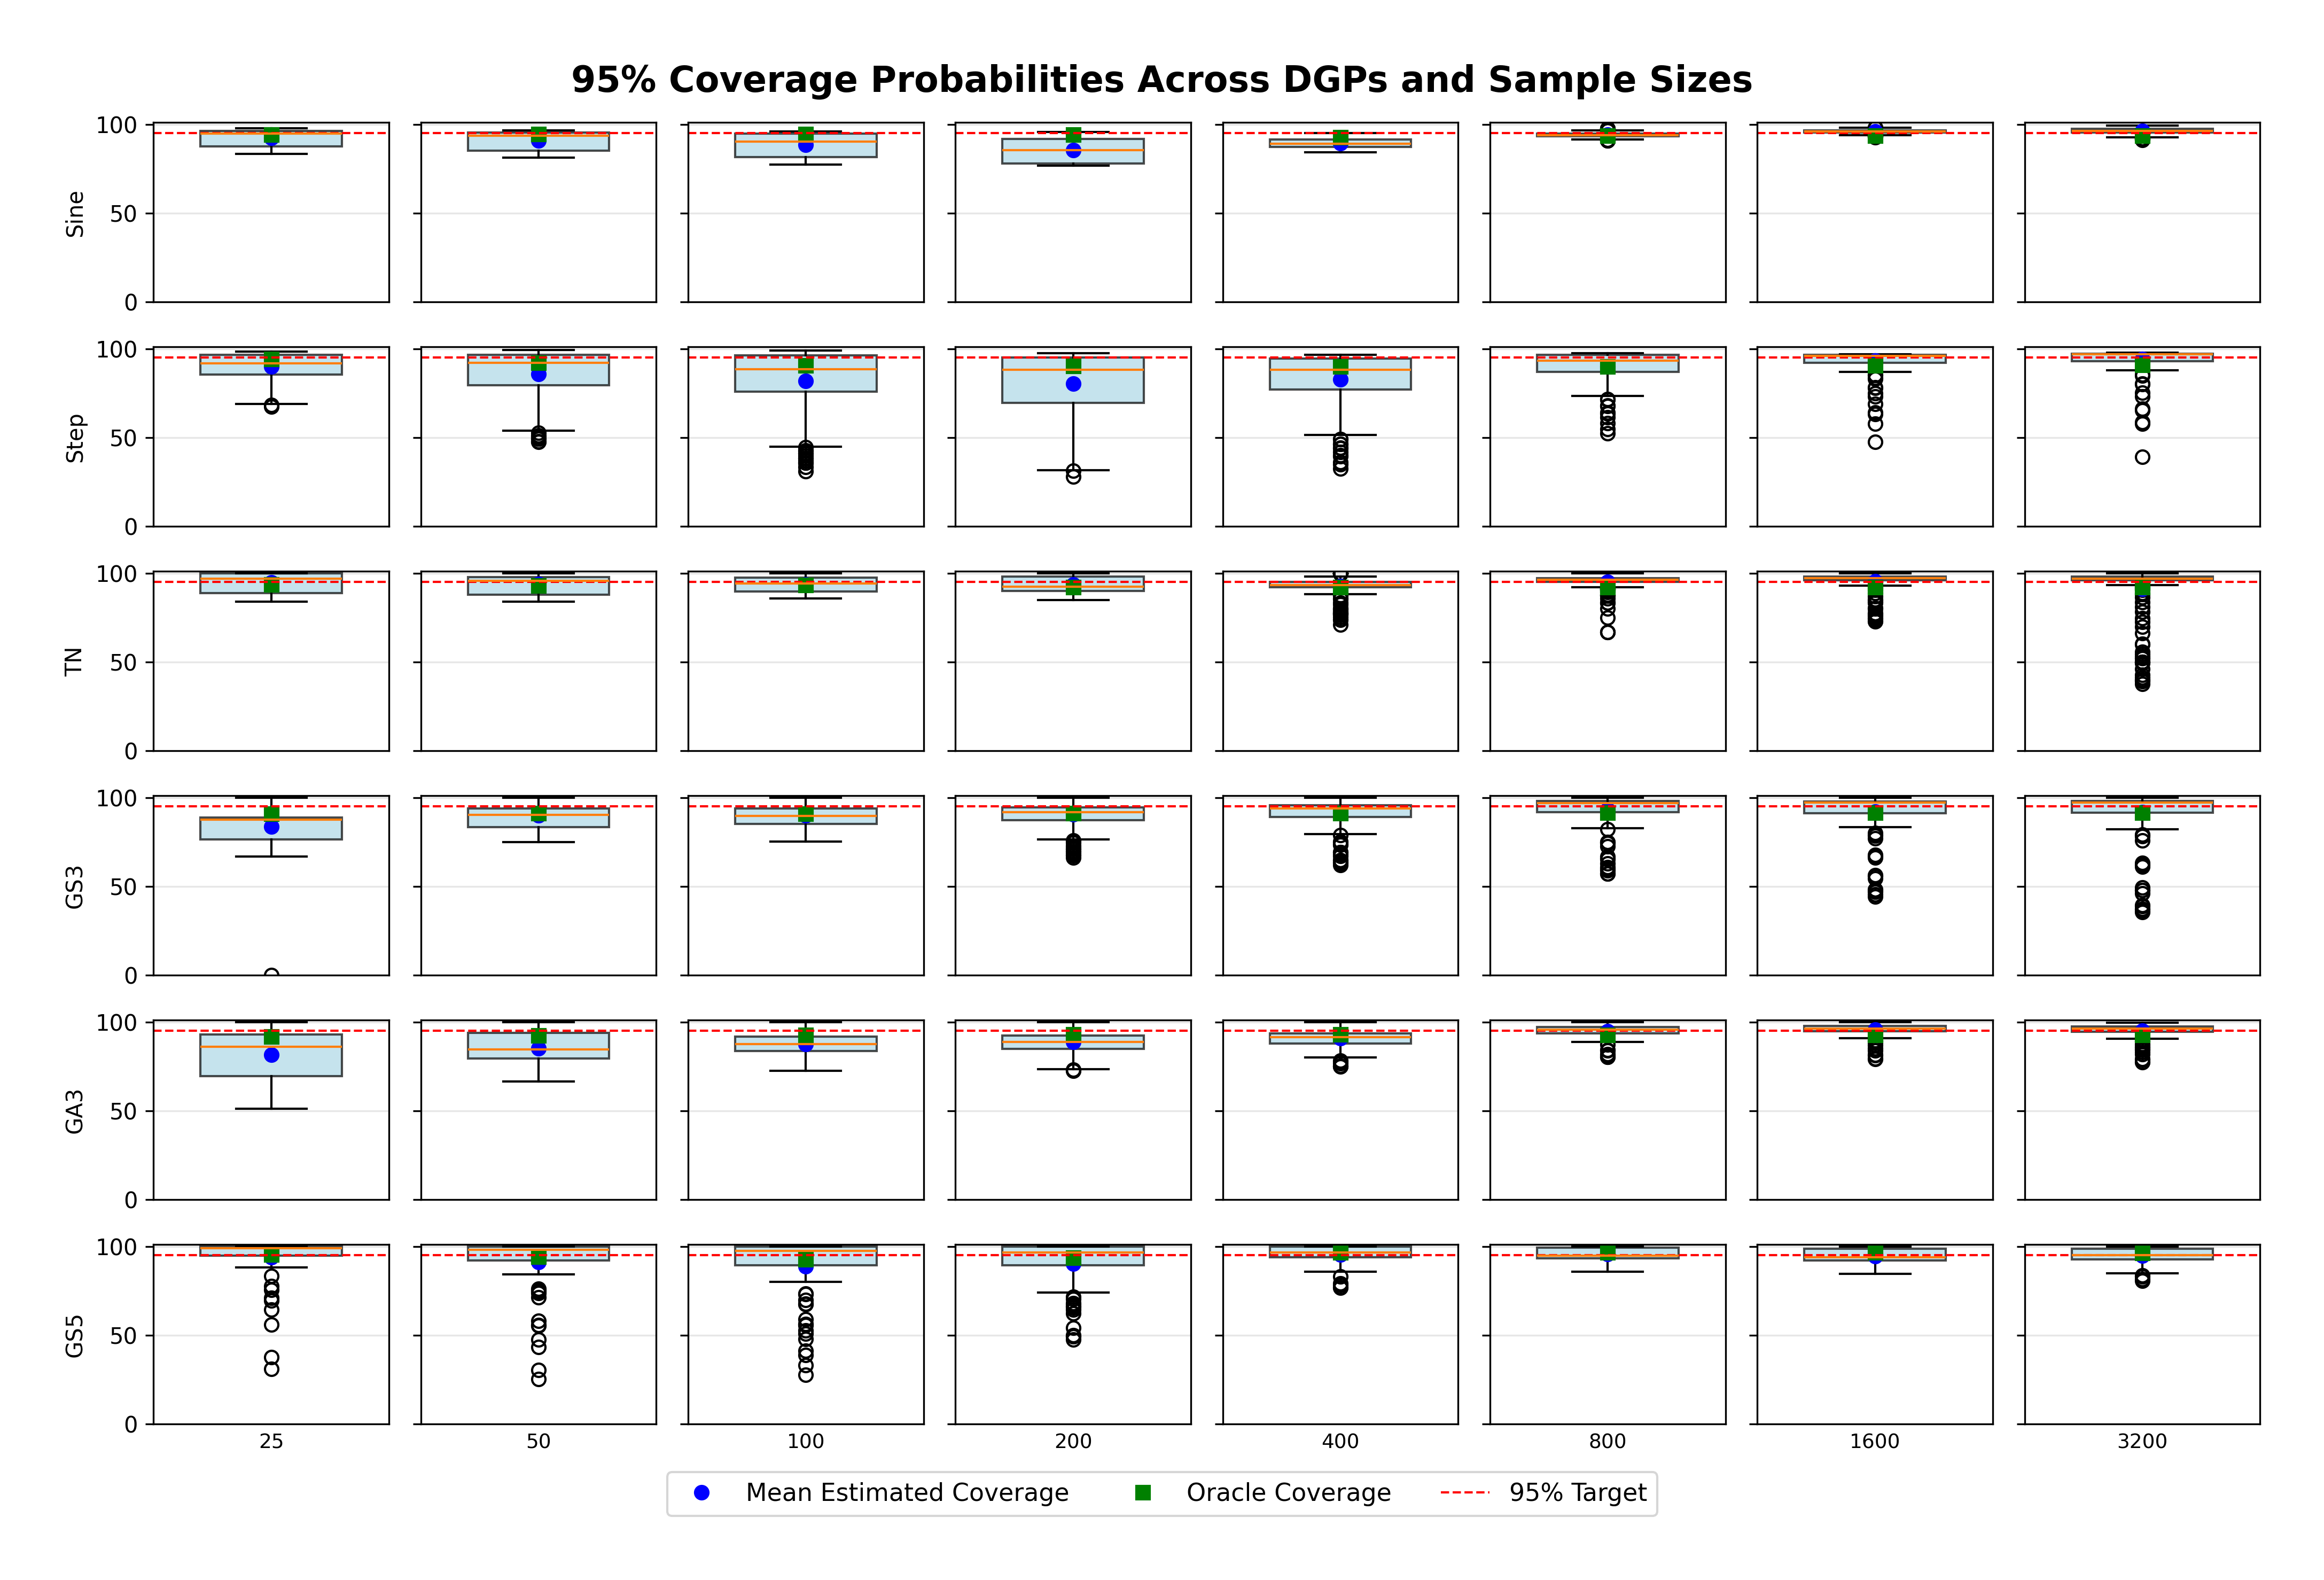
\includegraphics[angle=90, height=0.90\textheight]{resources/density_asymptotic_normality_and_var_est/Figure_Coverage_Combined.png}
    \caption{95\% coverage probabilities across DGPs and sample sizes (rotated for full\textendash page display).}
\end{figure}

\begin{figure}[p]
    \centering
    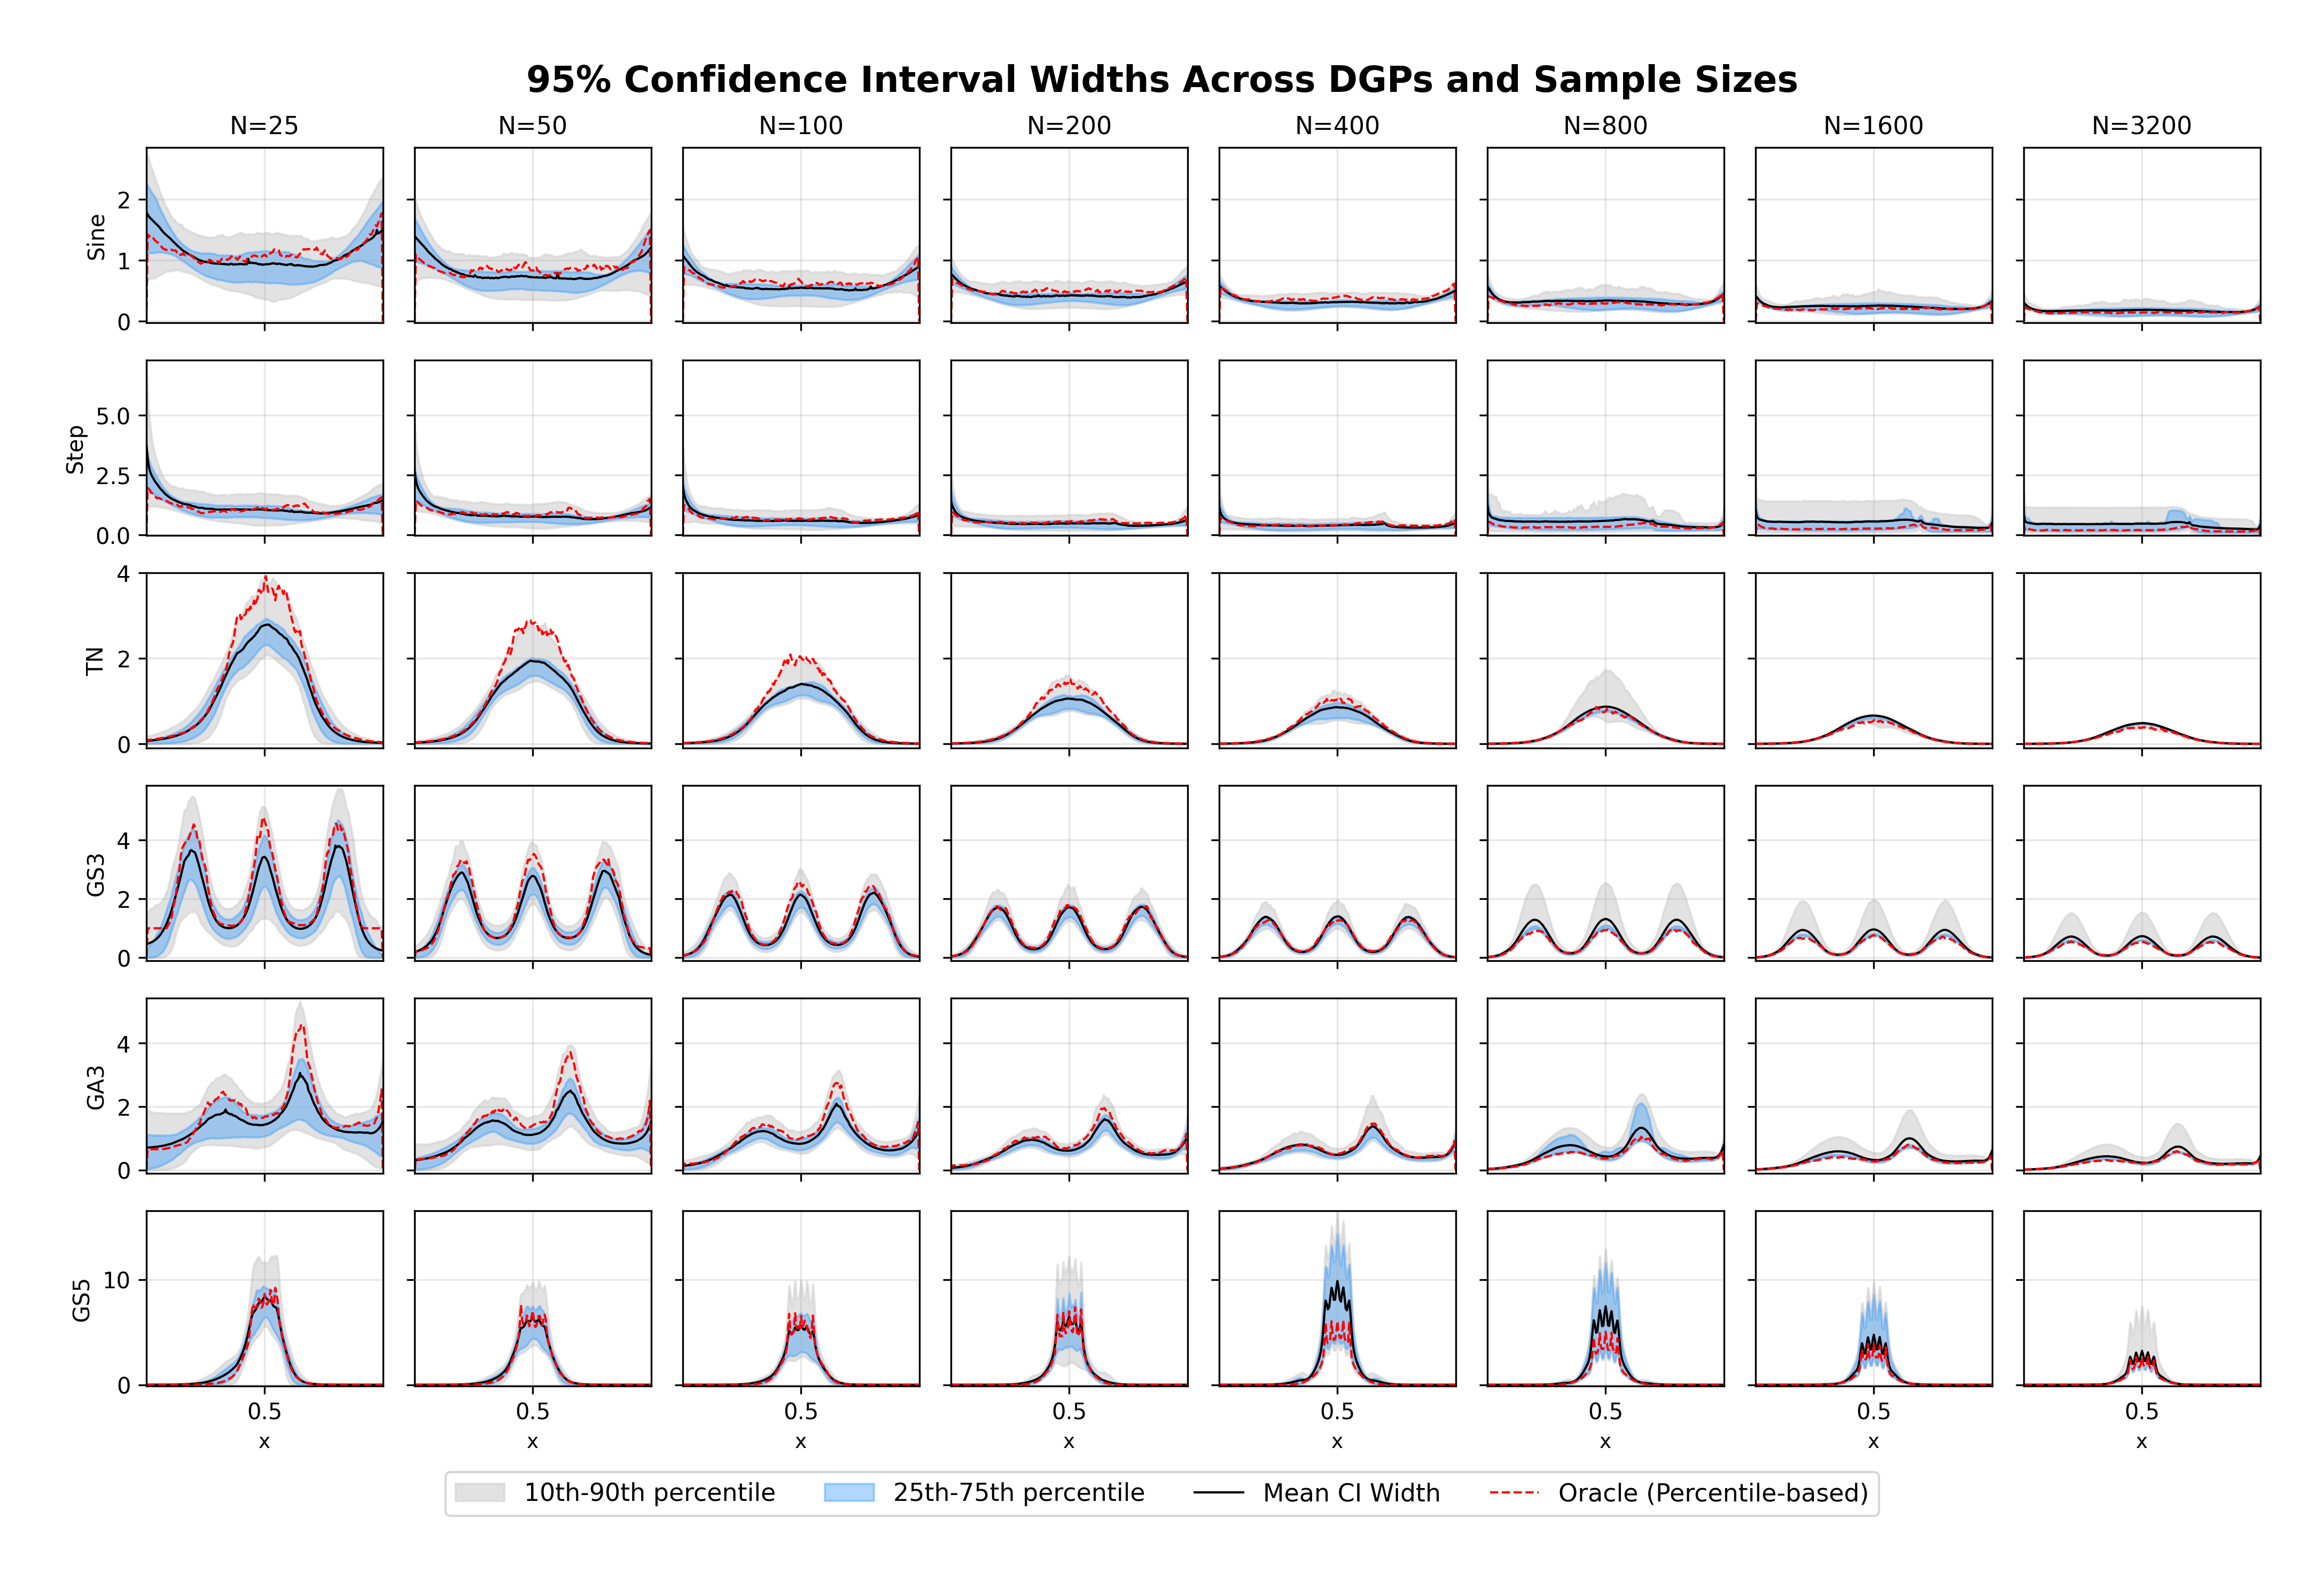
\includegraphics[angle=90, height=0.90\textheight]{resources/density_asymptotic_normality_and_var_est/Figure_CI_Widths_Combined.png}
    \caption{95\% confidence\textendash interval widths across DGPs and sample sizes (rotated for full\textendash page display).}
\end{figure}
\clearpage

\subsection{Asymptotic efficiency}\label{app_i_subsec:asymptotic_efficiency}
\begin{figure}[H]
    \centering
    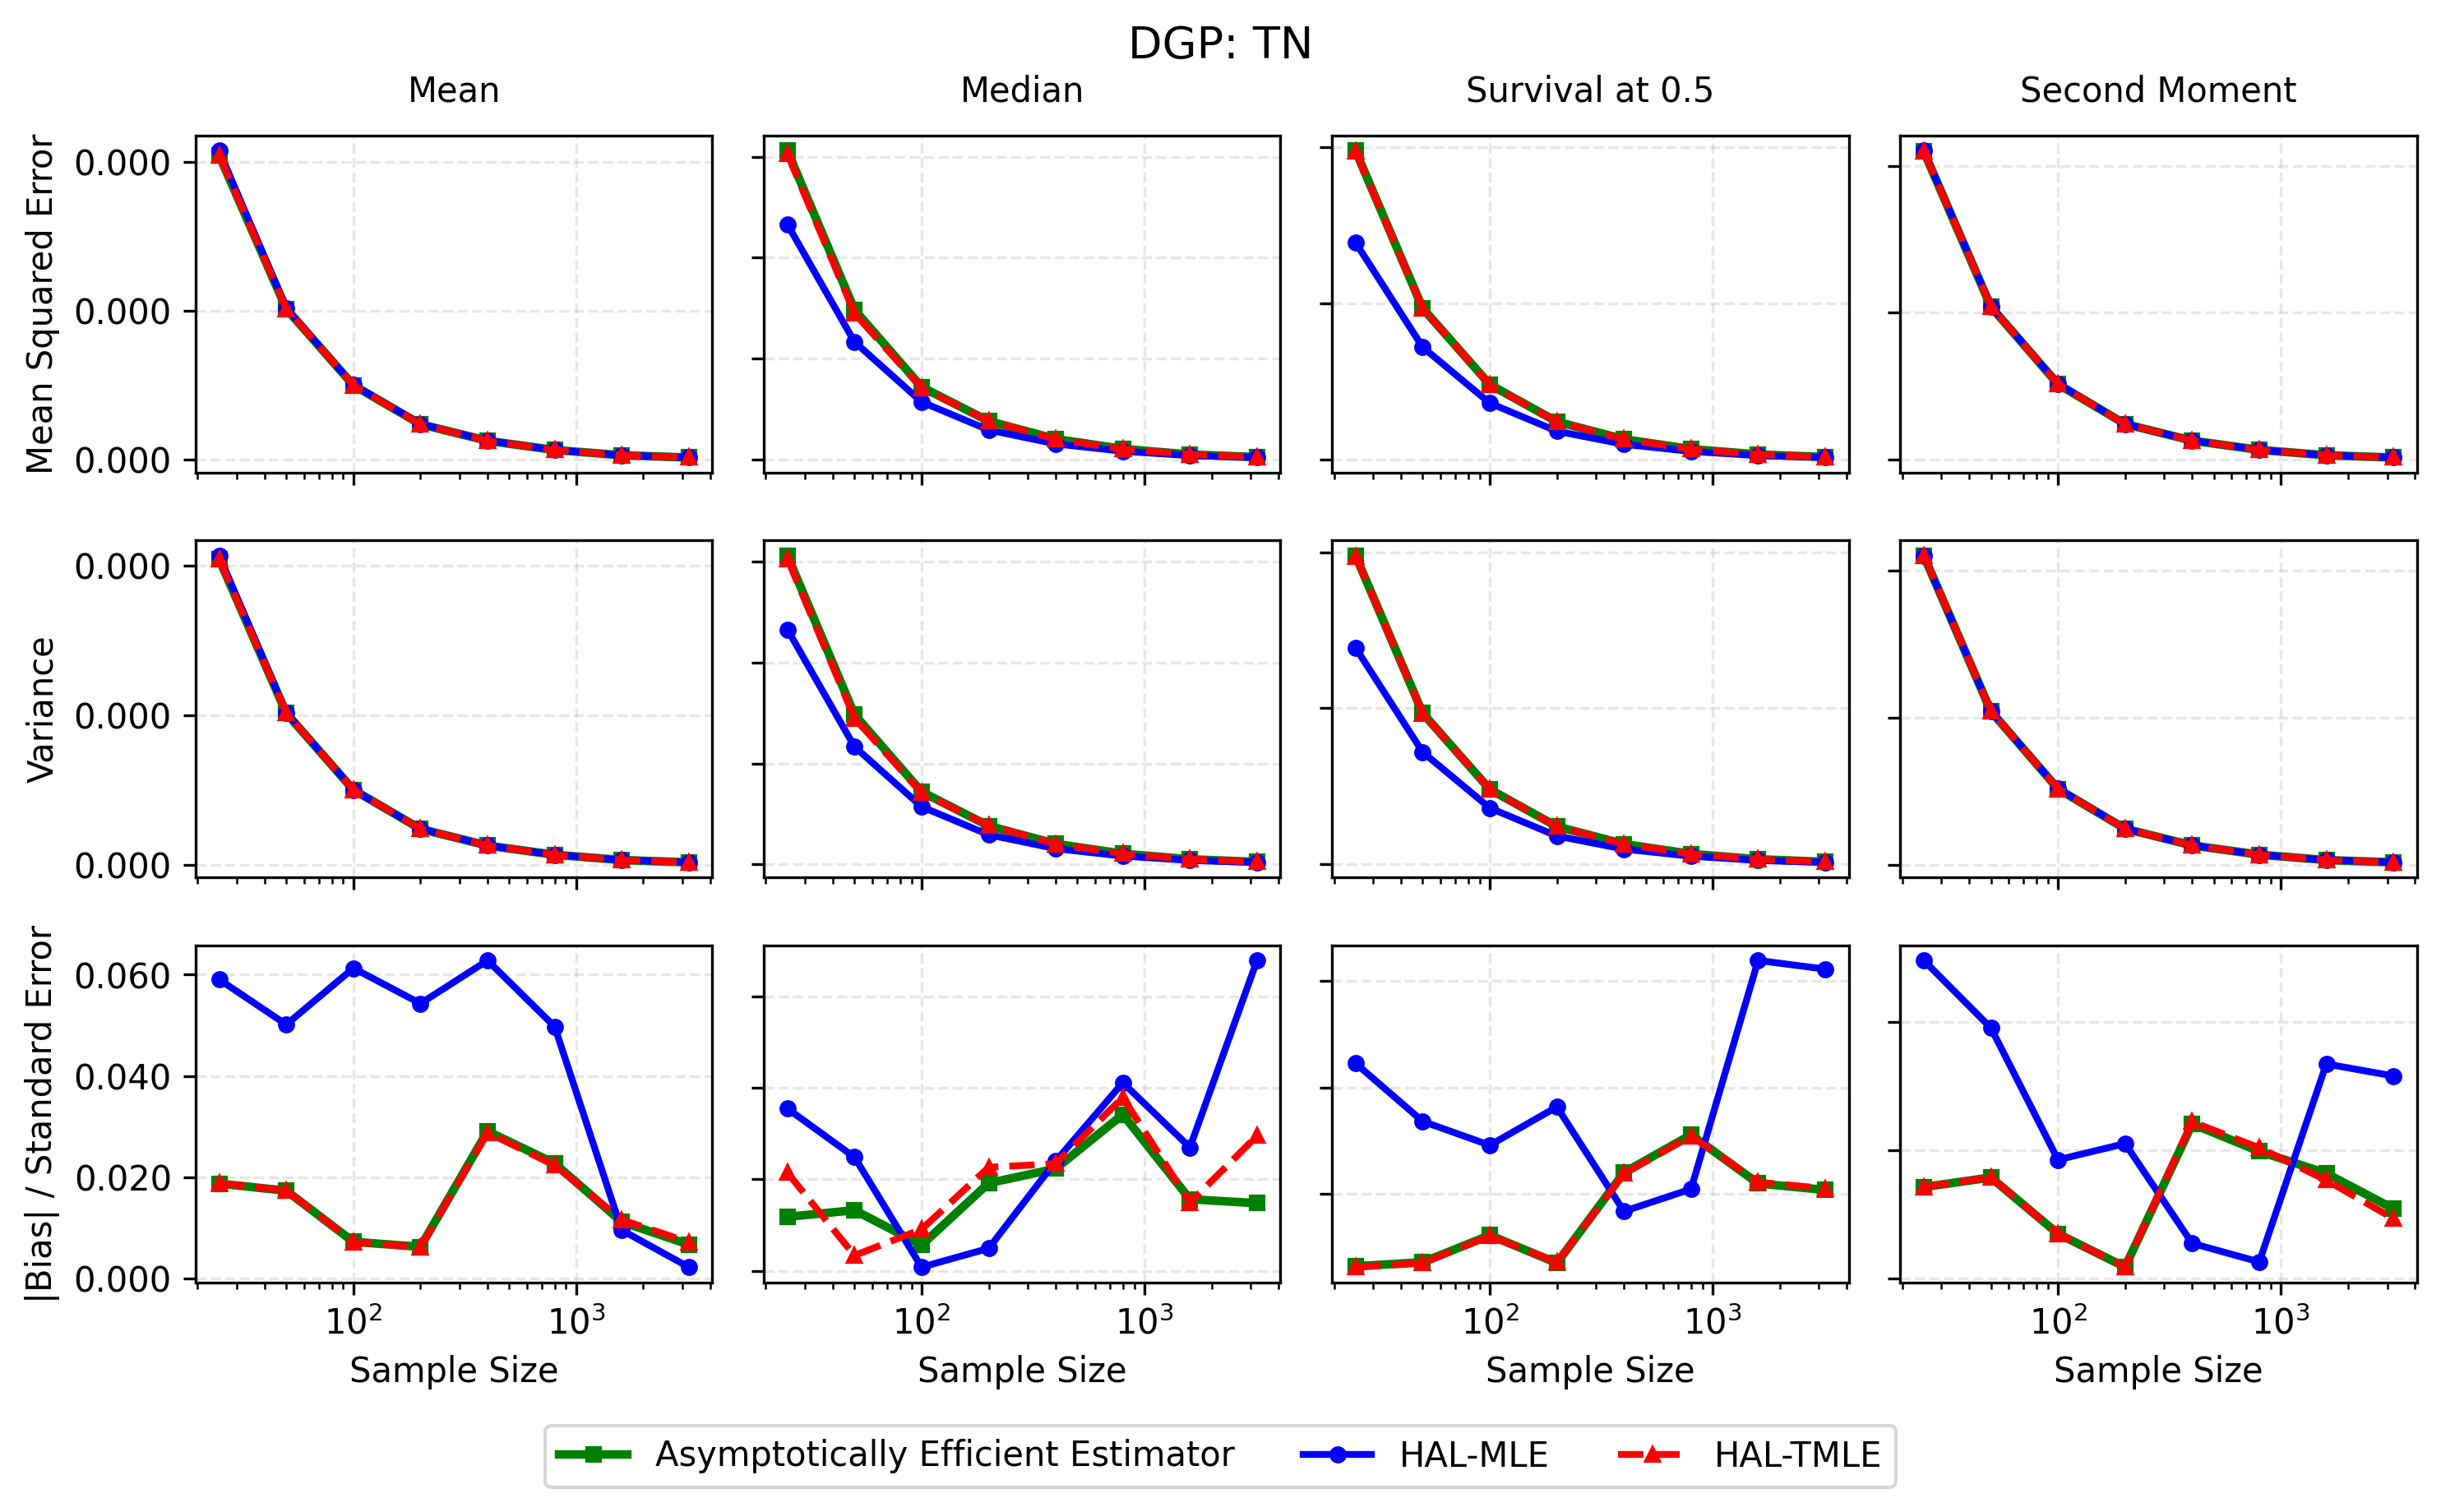
\includegraphics[width=0.9\textwidth]{resources/density_asymptotic_efficiency/TruncatedNormal/efficiency_comparison.png}
    \caption{Asymptotic\textendash efficiency comparison for TN.}
\end{figure}

\begin{figure}[H]
    \centering
    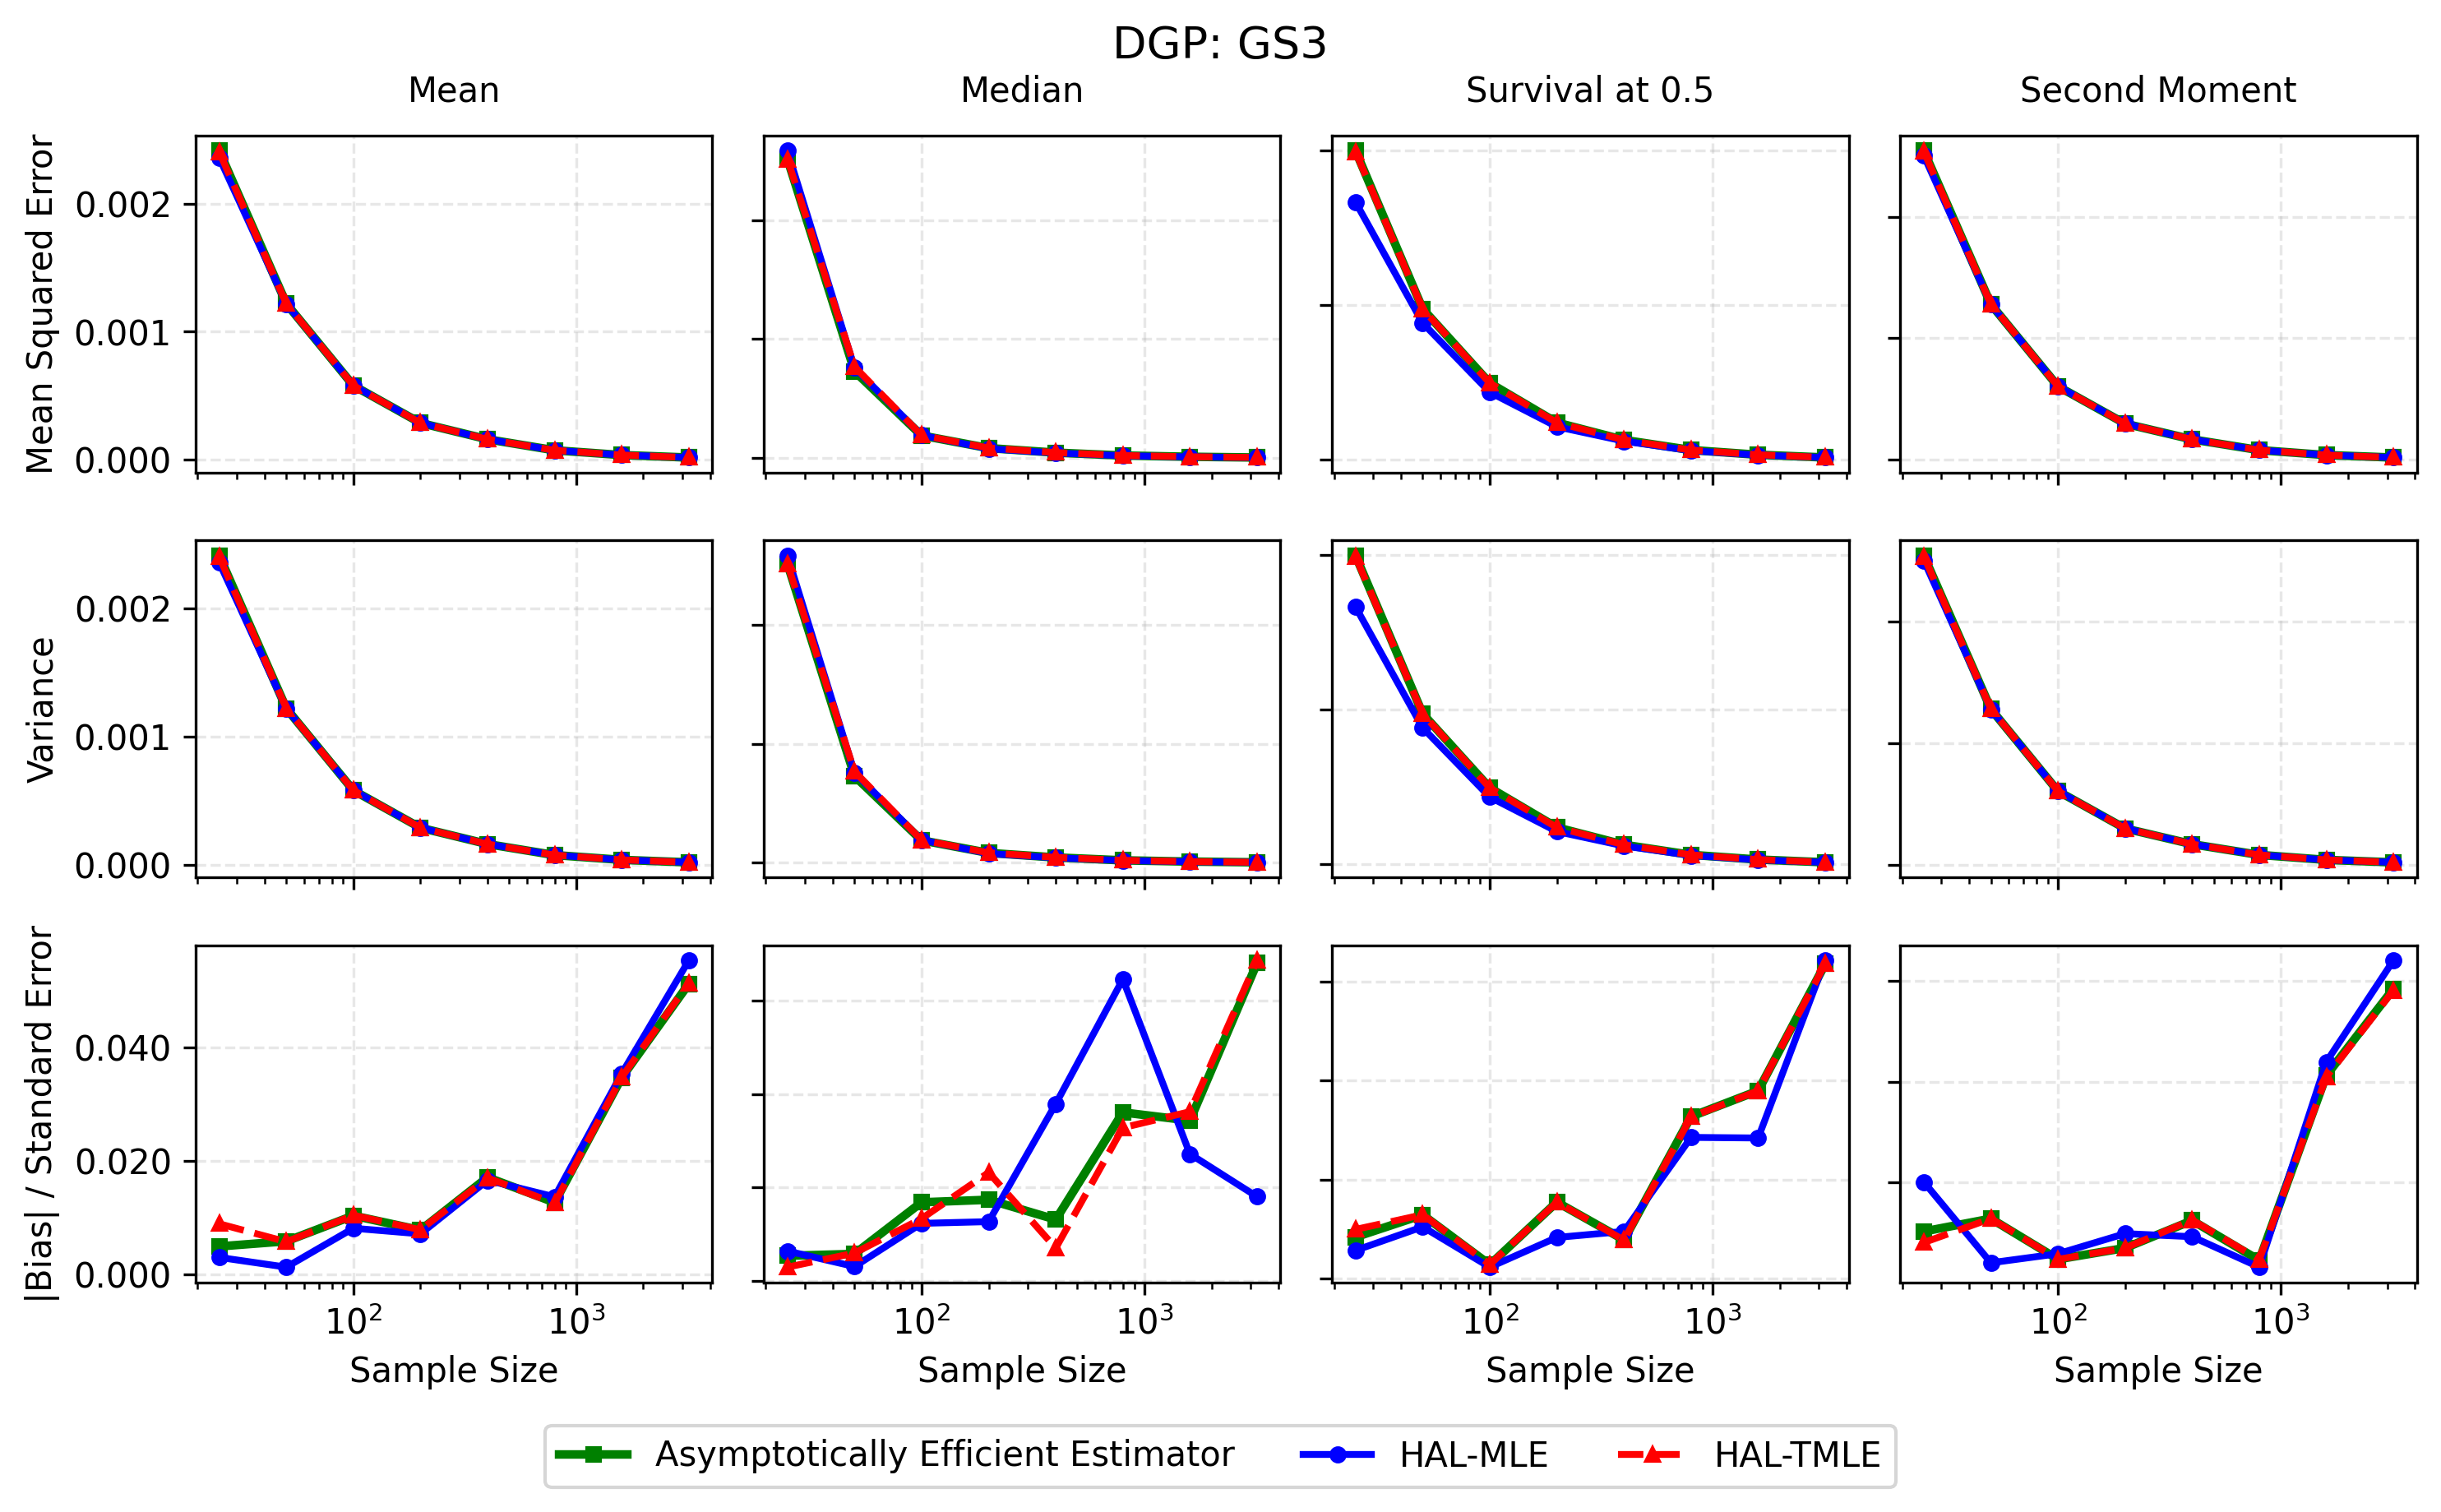
\includegraphics[width=0.9\textwidth]{resources/density_asymptotic_efficiency/TruncatedGMMSymmetricThree/efficiency_comparison.png}
    \caption{Asymptotic\textendash efficiency comparison for GS3.}
\end{figure}

\begin{figure}[H]
    \centering
    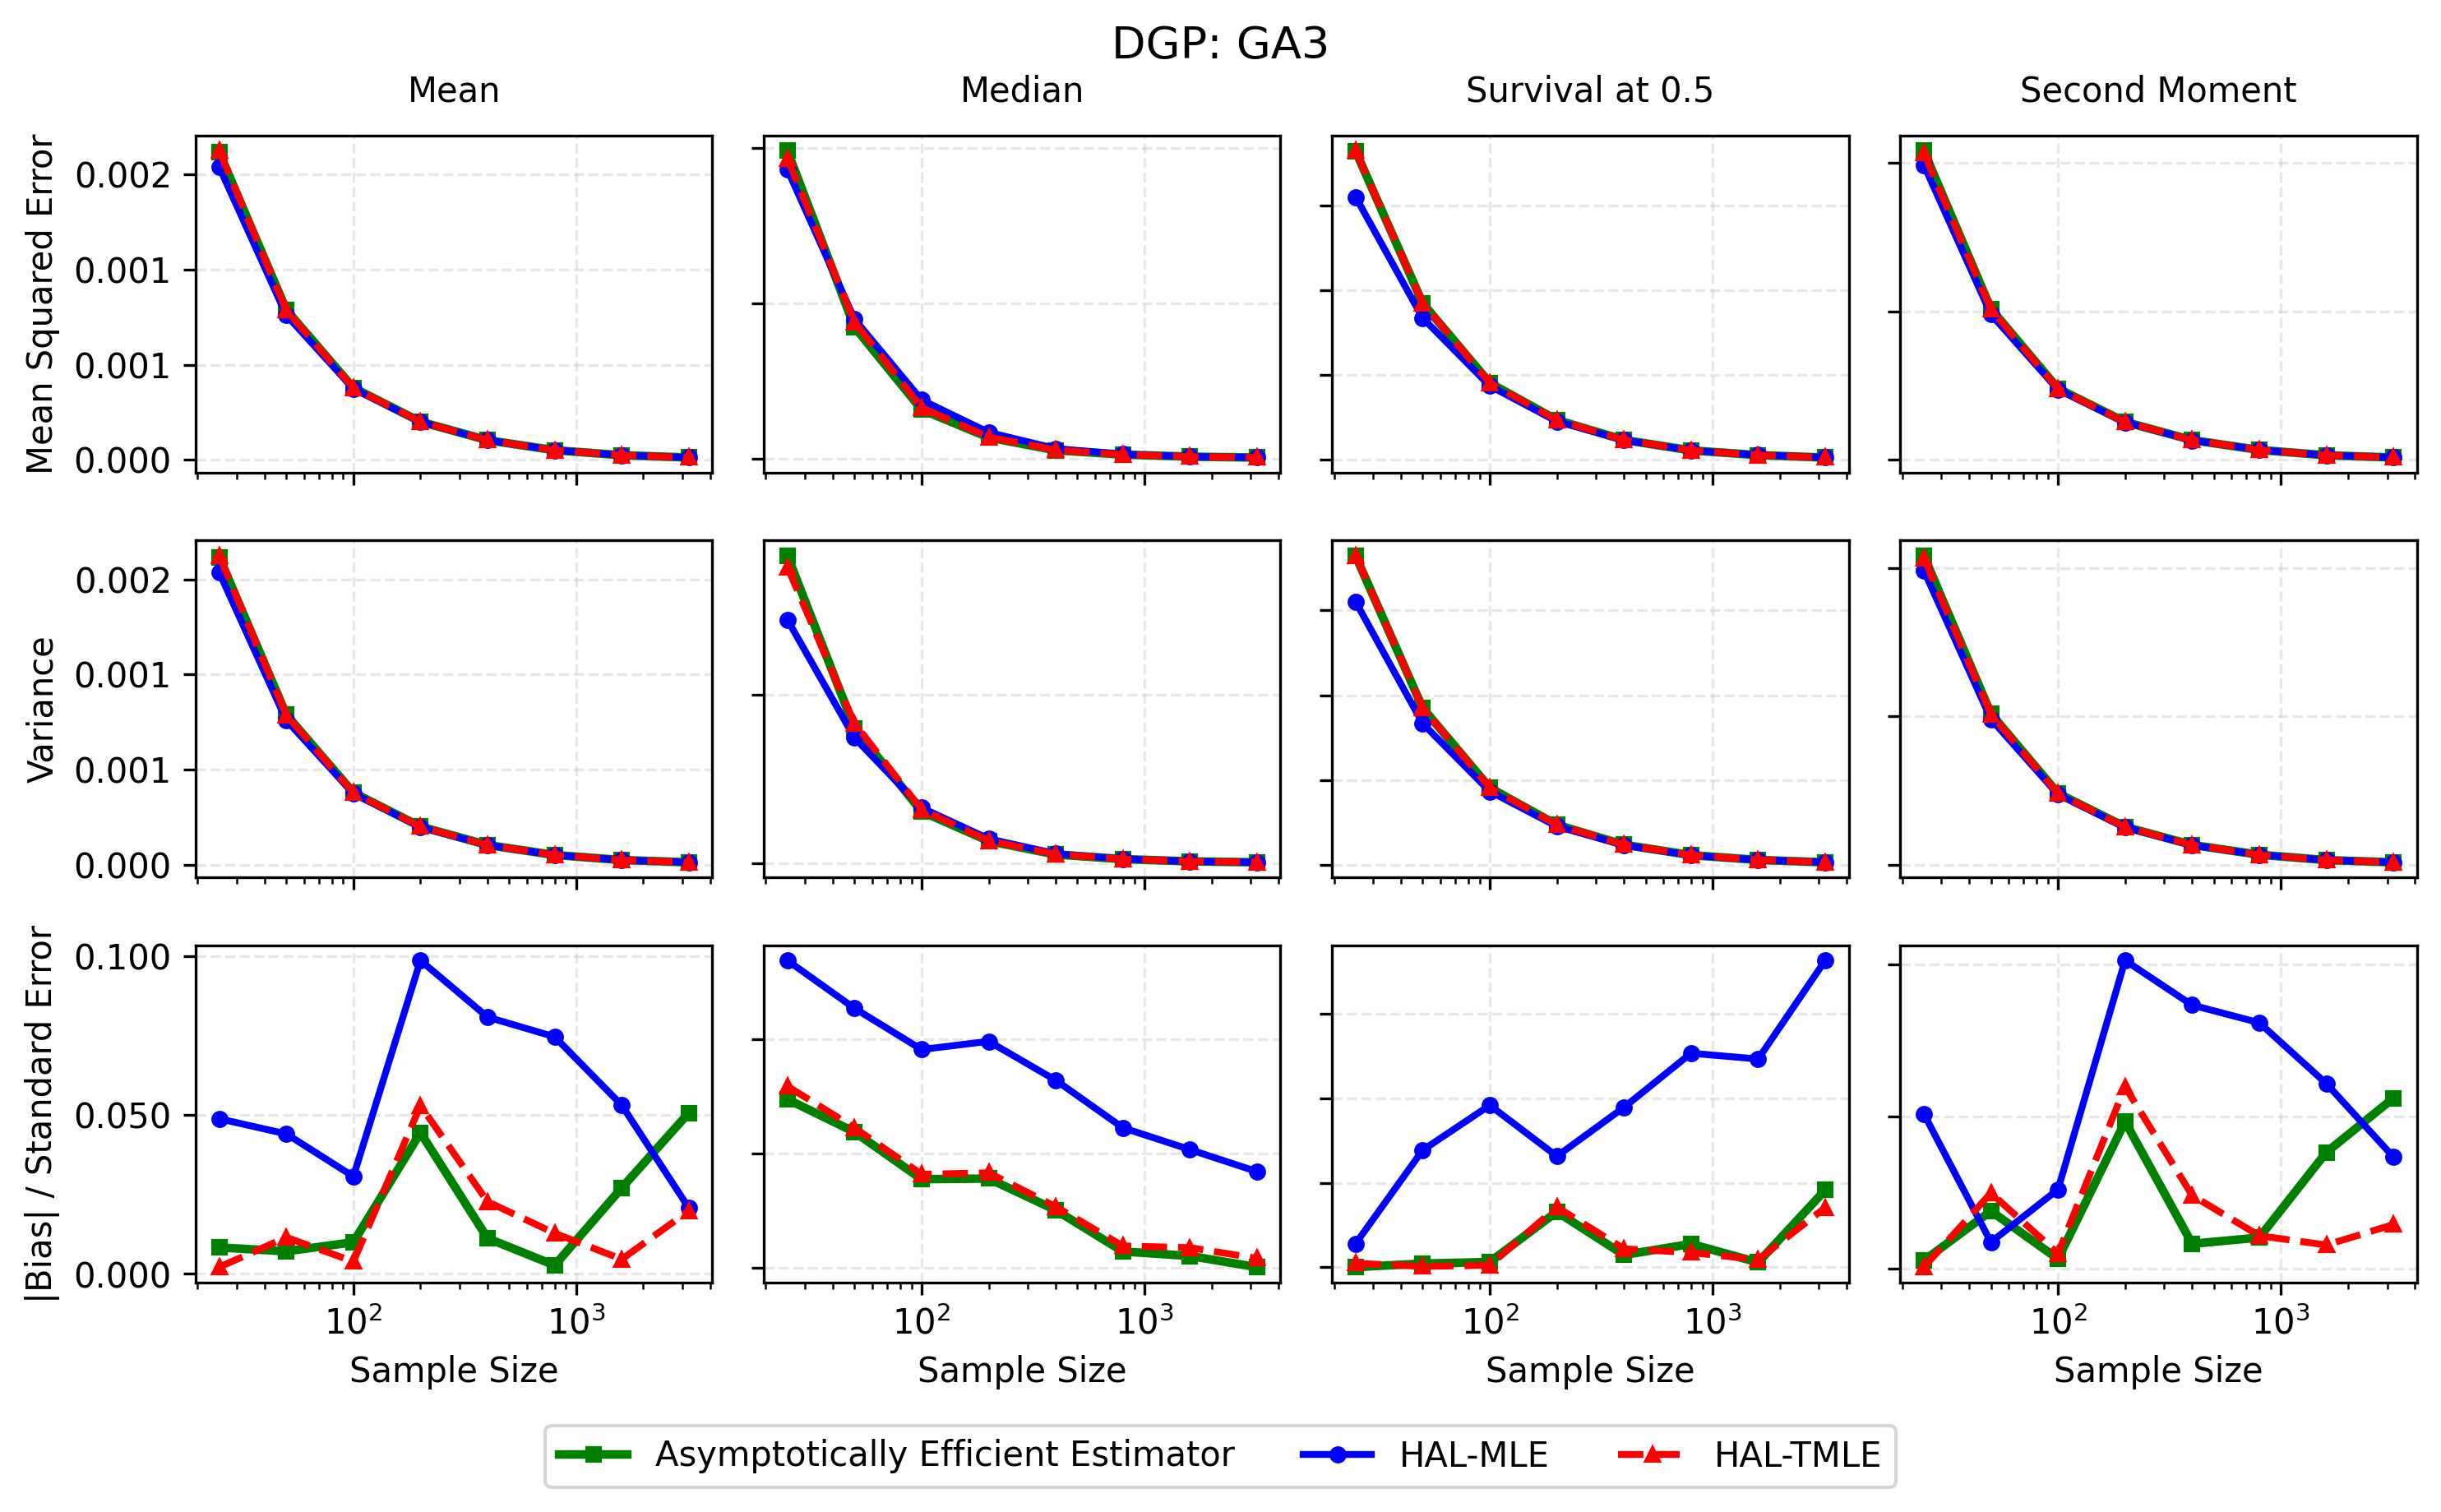
\includegraphics[width=0.9\textwidth]{resources/density_asymptotic_efficiency/TruncatedGMMAsymmetricThree/efficiency_comparison.png}
    \caption{Asymptotic\textendash efficiency comparison for GA3.}
\end{figure}

\begin{figure}[H]
    \centering
    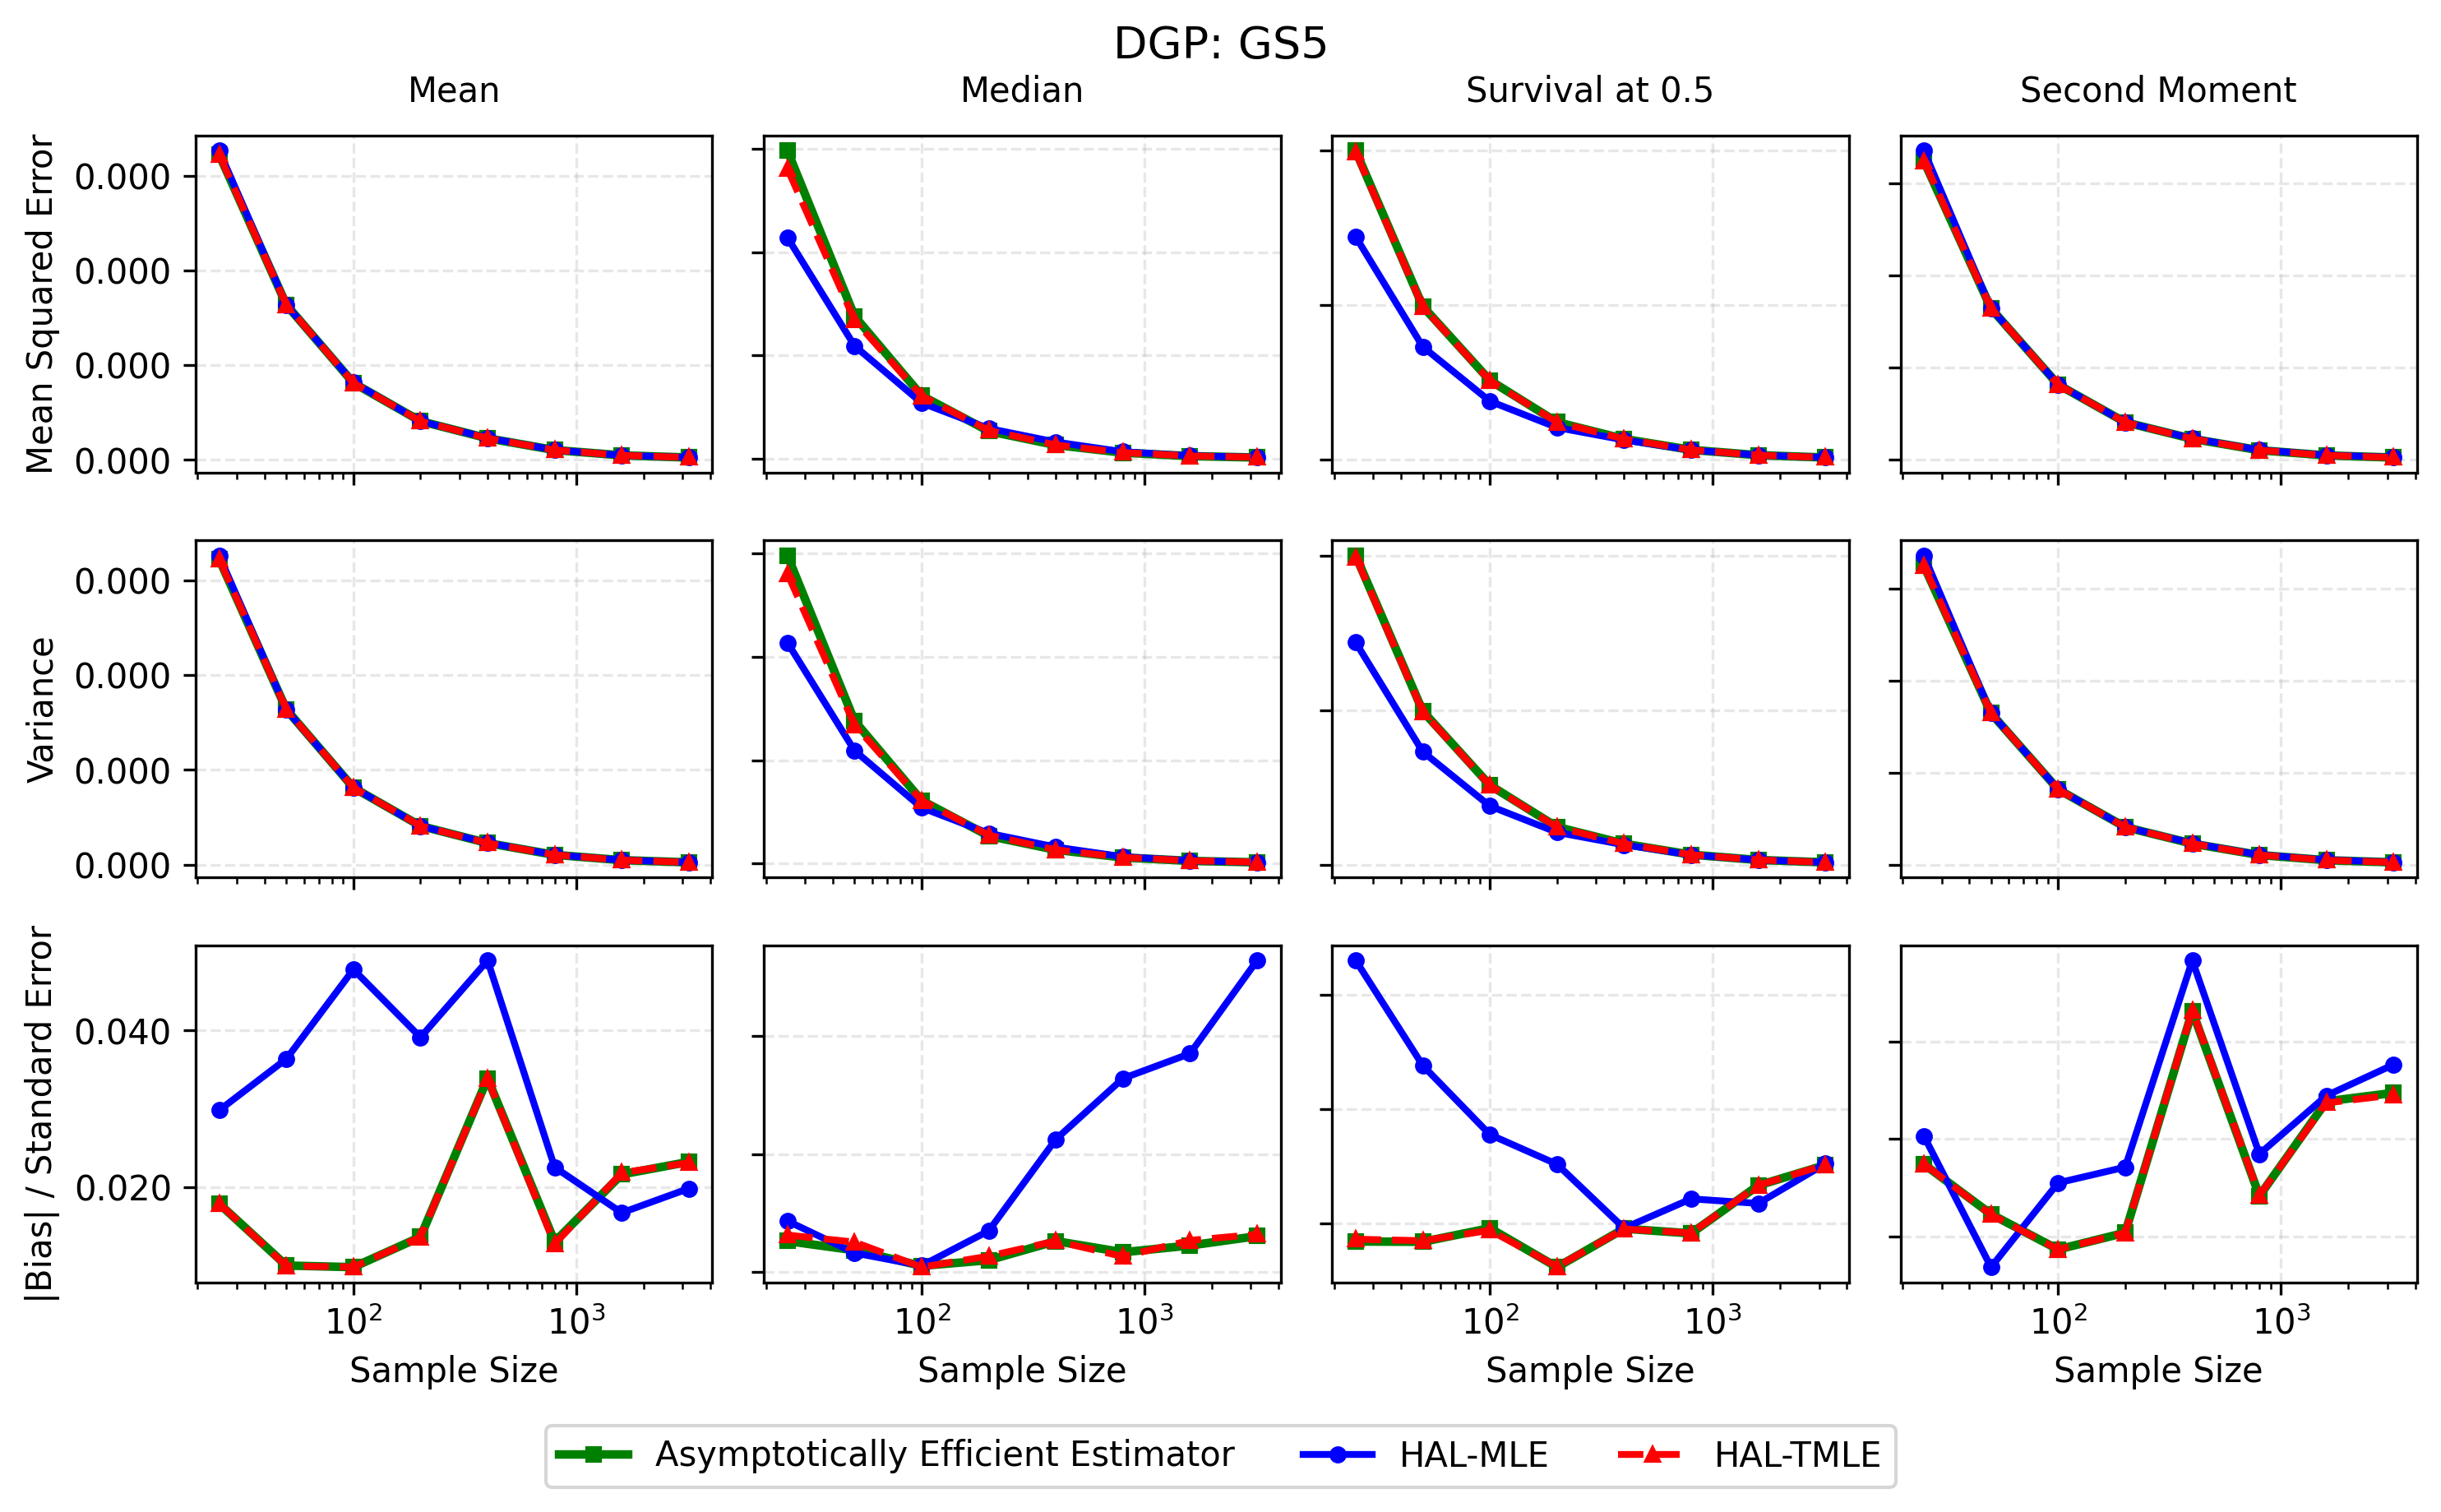
\includegraphics[width=0.9\textwidth]{resources/density_asymptotic_efficiency/TruncatedGMMFiveSpikes/efficiency_comparison.png}
    \caption{Asymptotic\textendash efficiency comparison for GS5.}
\end{figure}

\begin{figure}[H]
    \centering
    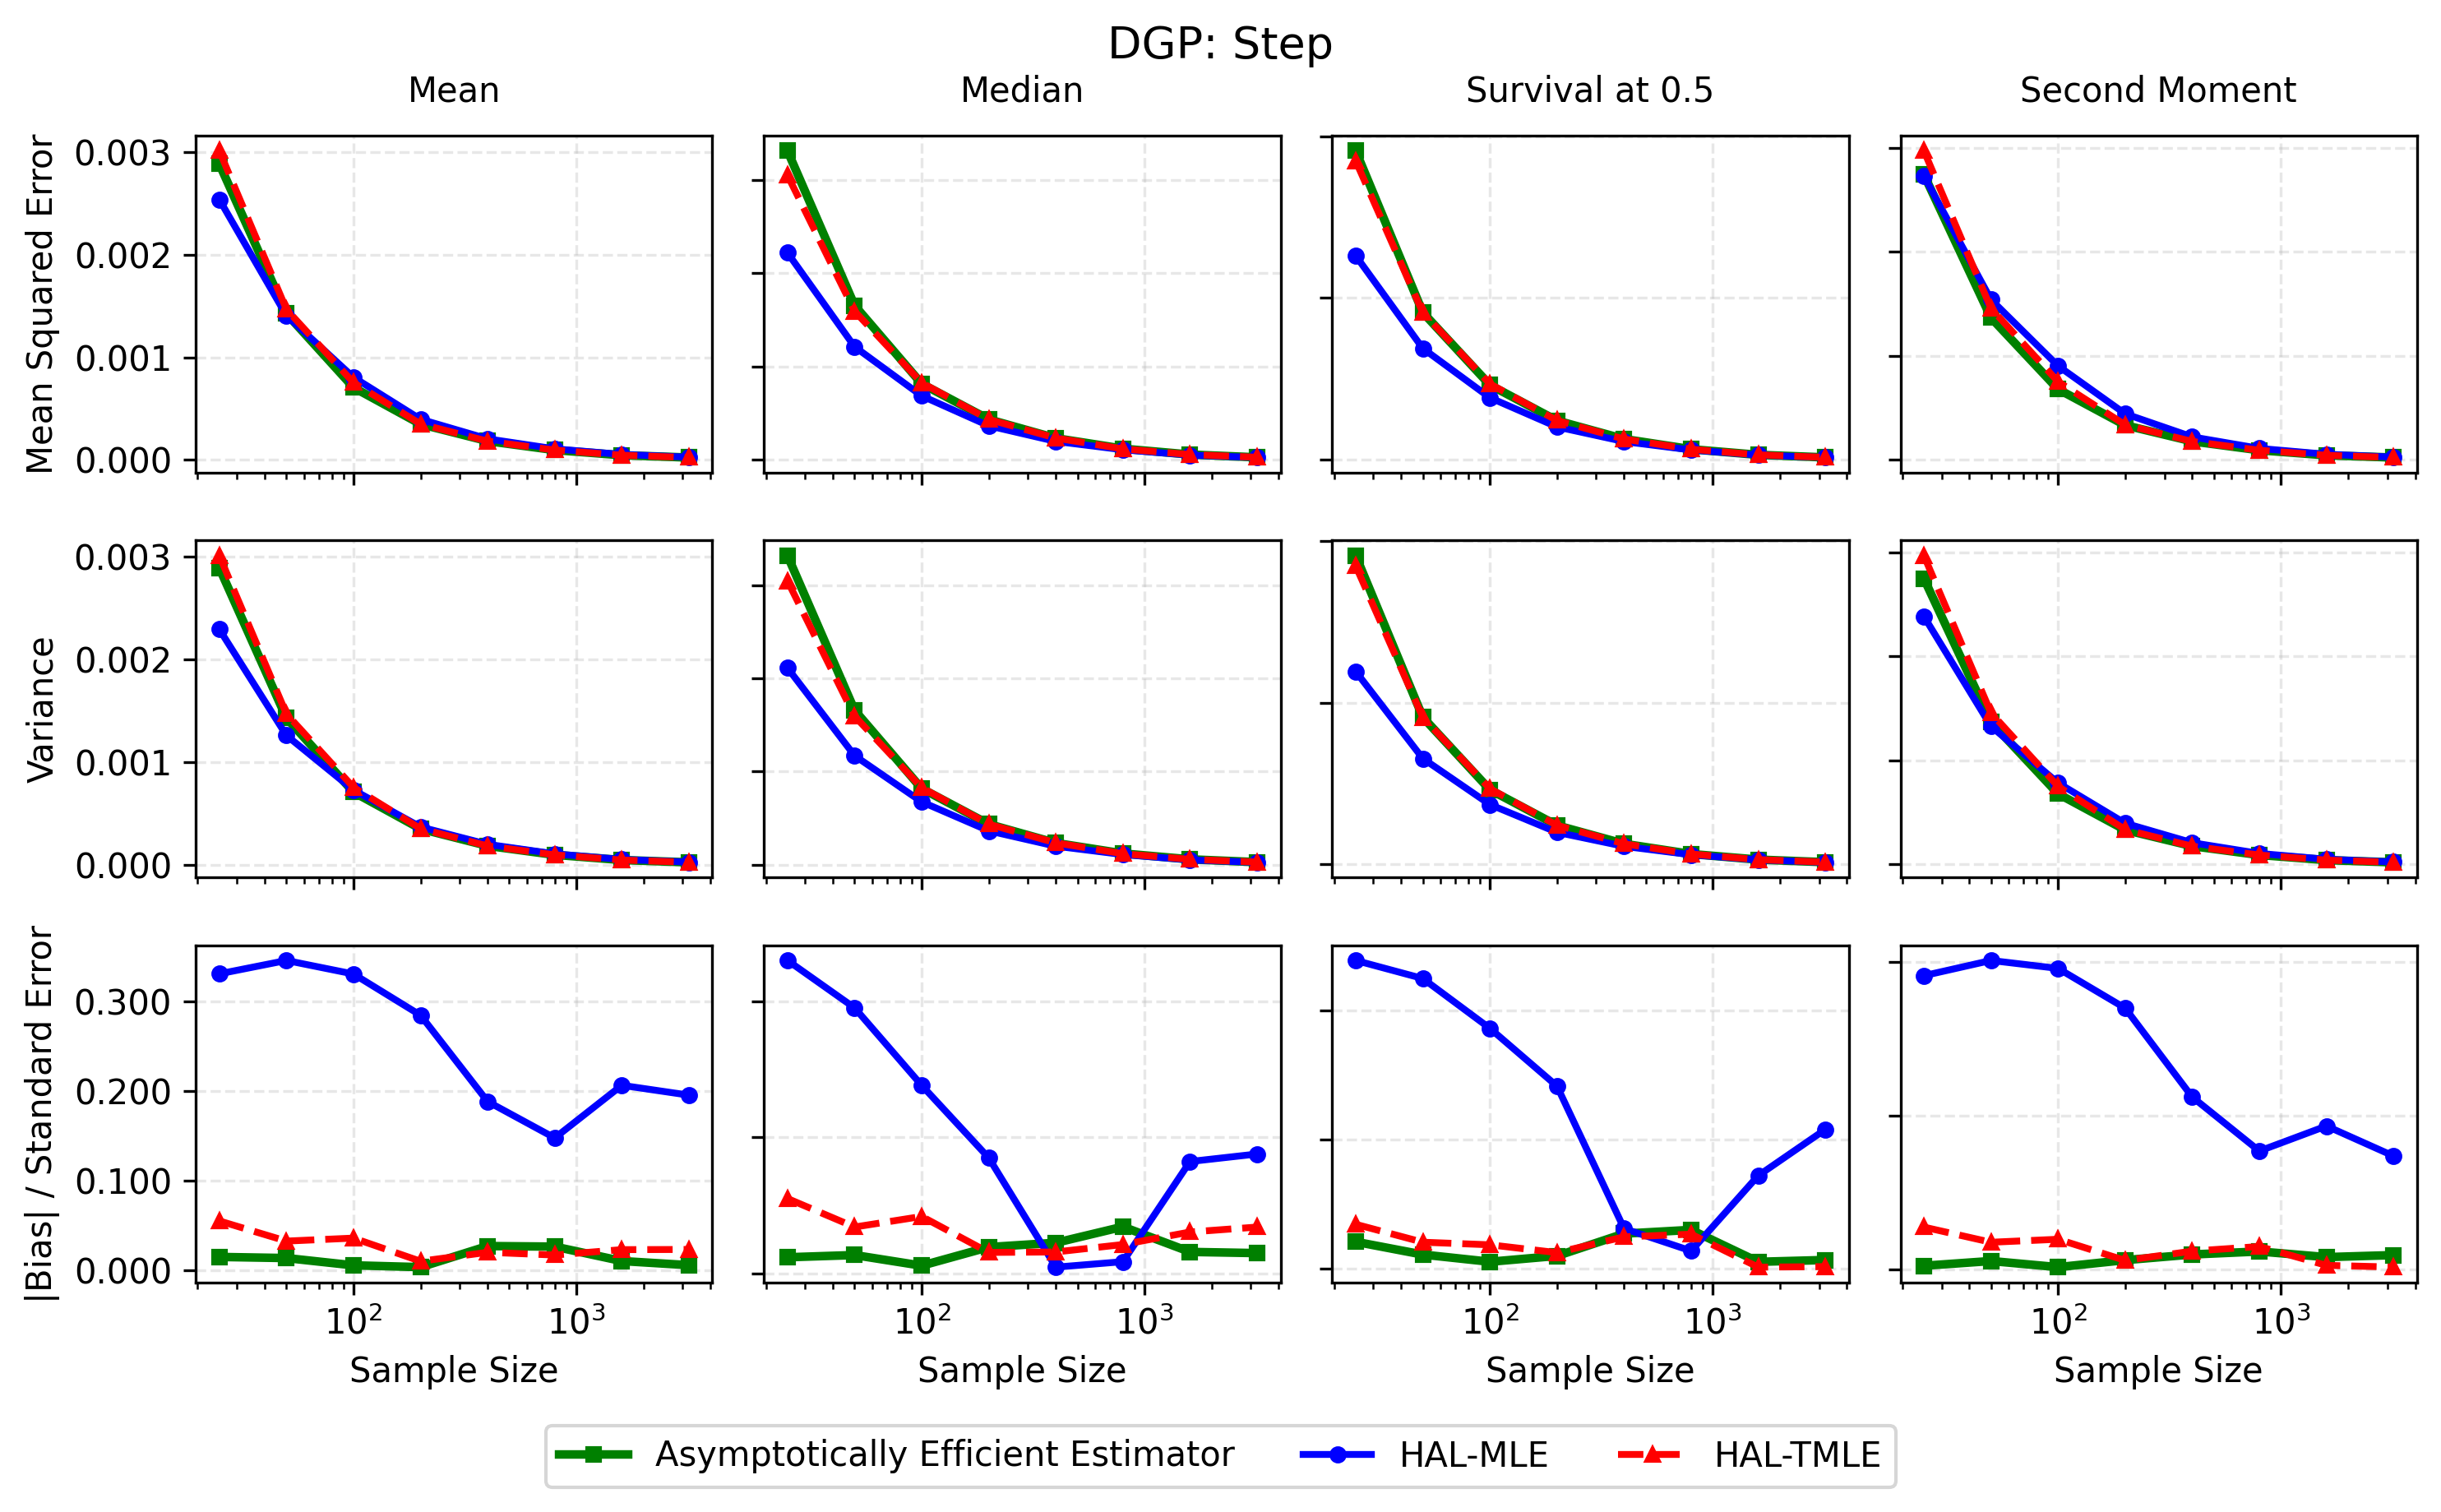
\includegraphics[width=0.9\textwidth]{resources/density_asymptotic_efficiency/StepFunction/efficiency_comparison.png}
    \caption{Asymptotic\textendash efficiency comparison for Step.}
\end{figure}

\begin{figure}[H]
    \centering
    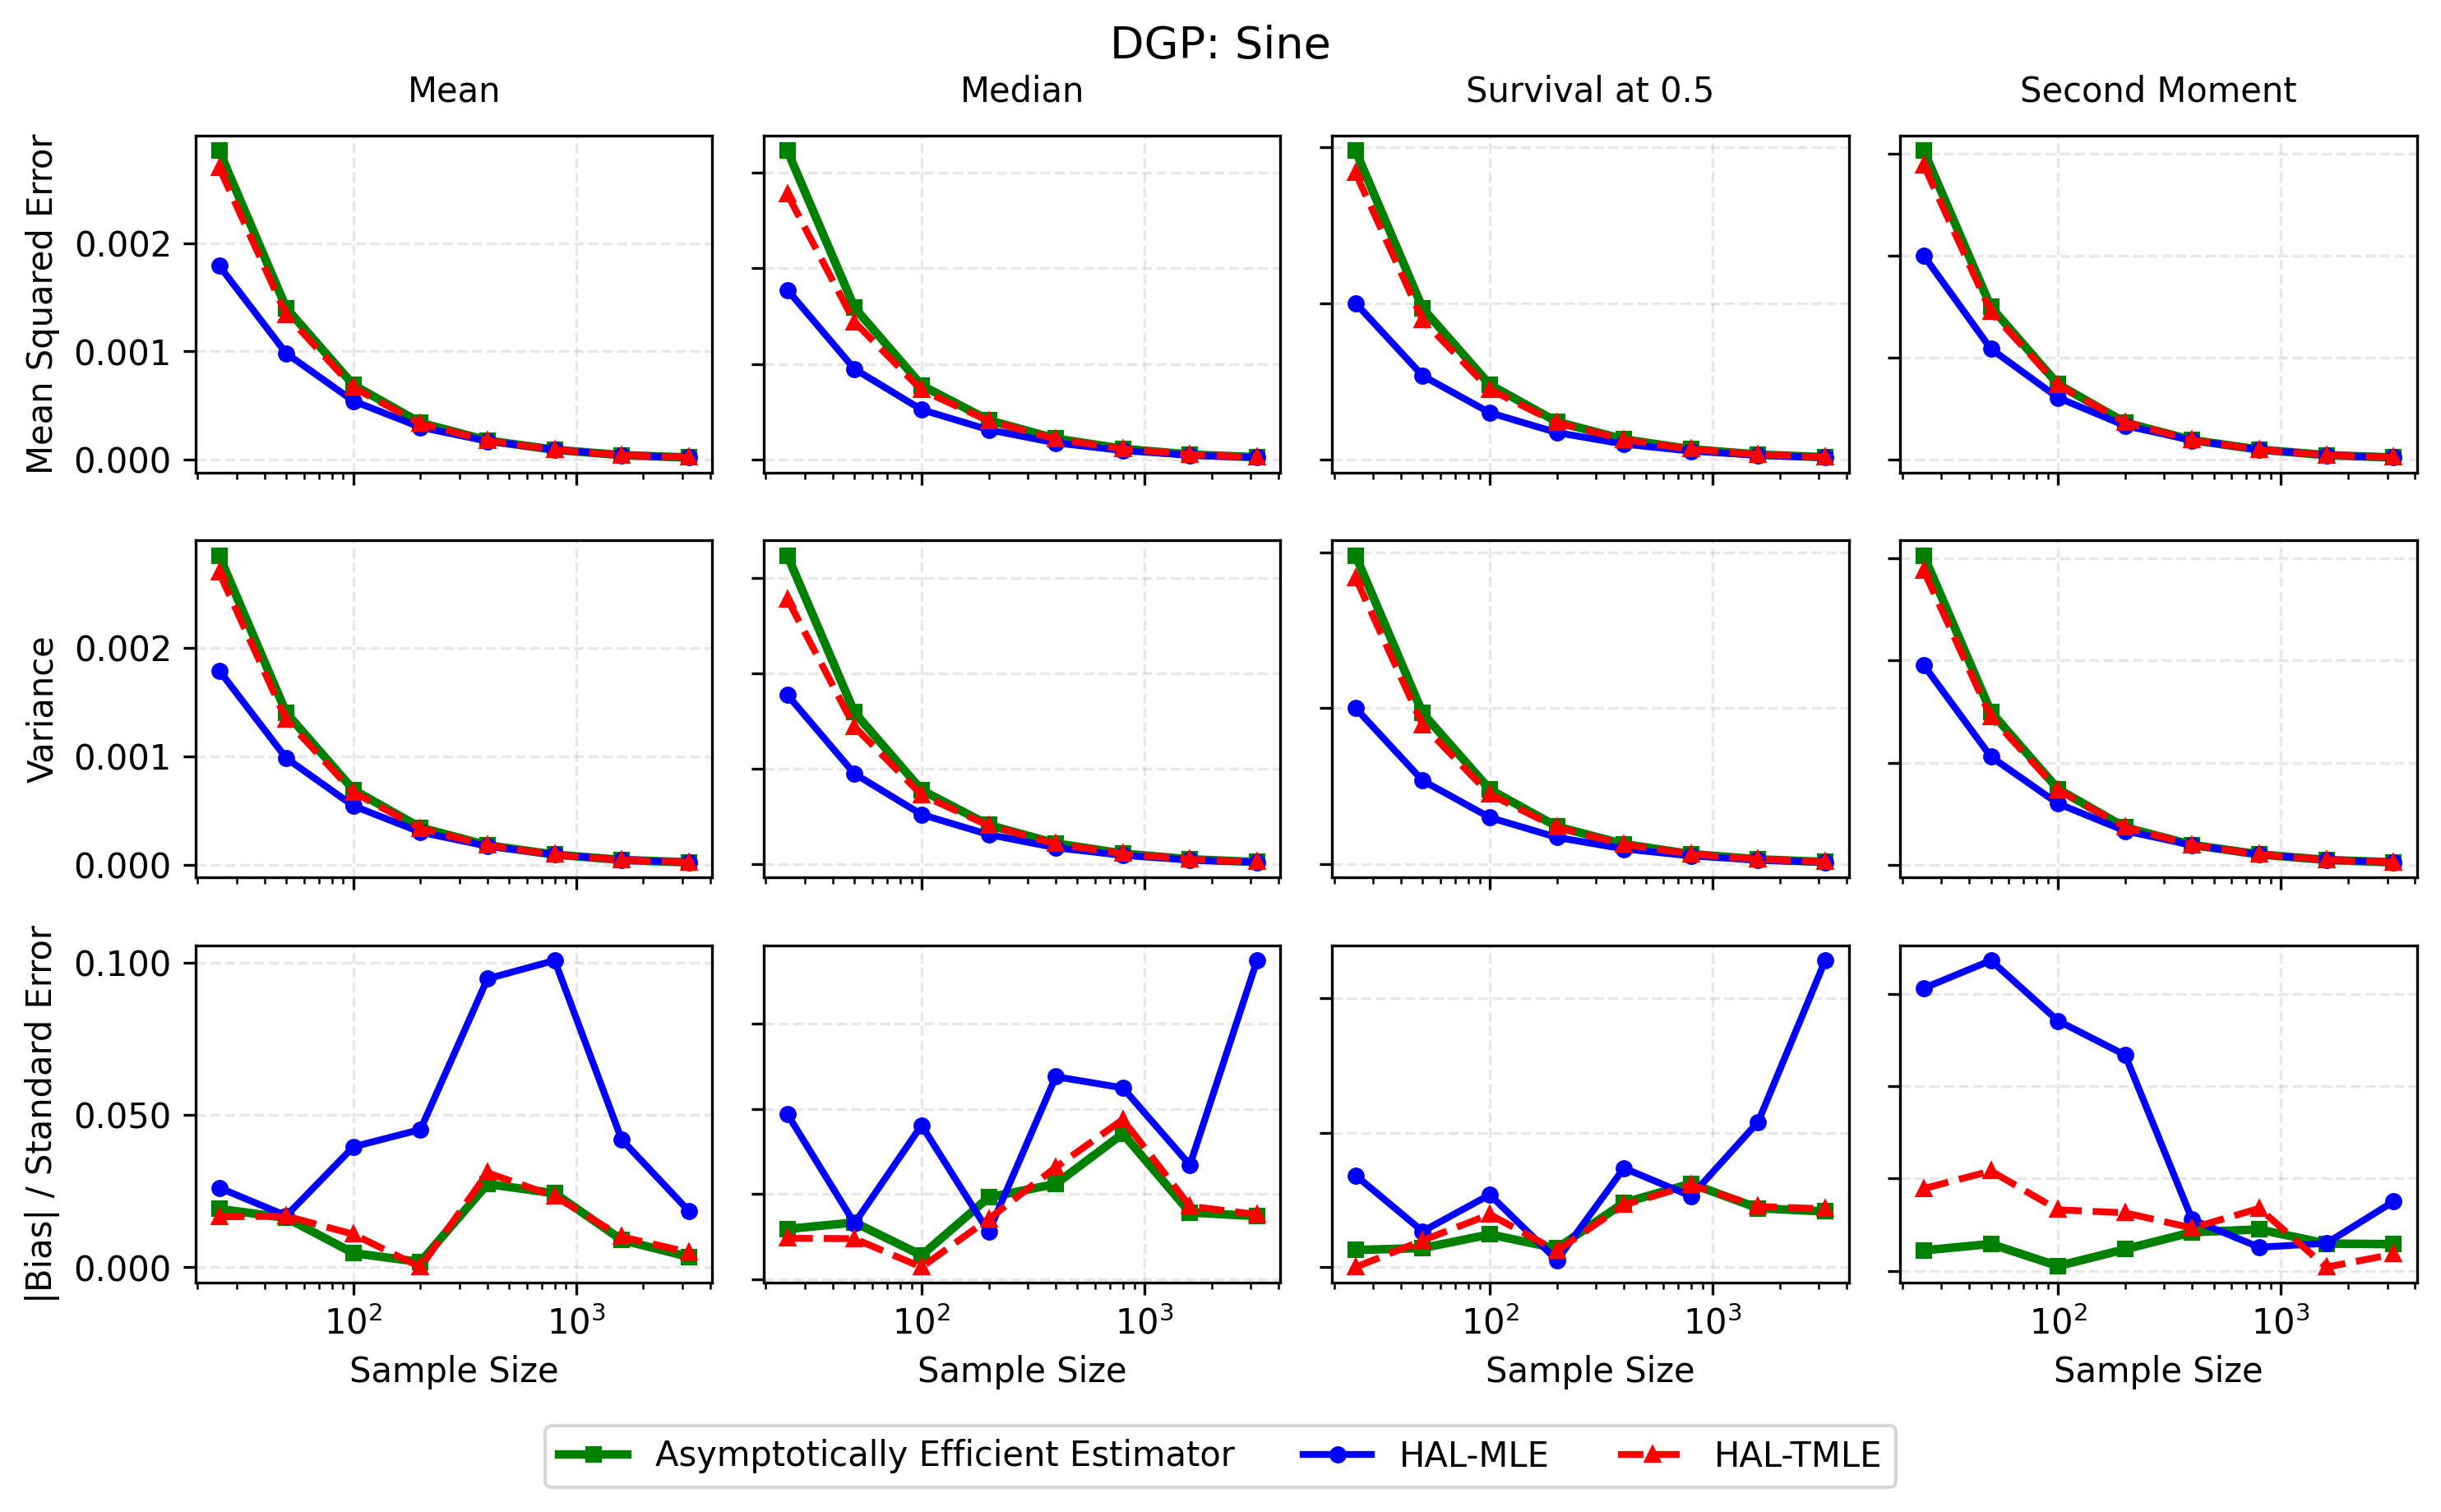
\includegraphics[width=0.9\textwidth]{resources/density_asymptotic_efficiency/Sinusoidal/efficiency_comparison.png}
    \caption{Asymptotic\textendash efficiency comparison for Sine.}
\end{figure}

\clearpage
\subsection{EIC\textendash based variance estimation for statistical estimands}\label{app_i_subsec:eic-based-variance-estimation}

% Auto-generated targeting coverage analysis table
\begin{table}[H]
  \centering
  \scriptsize
  \setlength{\tabcolsep}{2pt}
  \renewcommand{\arraystretch}{1.1}
  \begin{tabular}{lcccccccc}
    \toprule
    DGP & N=25 & N=50 & N=100 & N=200 & N=400 & N=800 & N=1600 & N=3200 \\
    \midrule
    TN & (93.3, 94.6) & (94.4, 96.0) & (94.9, 95.2) & (95.8, 95.4) & (94.7, 94.7) & (93.9, 95.1) & (95.3, 95.2) & (94.3, 94.3) \\
    GS3 & (95.1, 95.9) & (95.2, 95.8) & (95.7, 95.9) & (95.5, 94.9) & (94.3, 95.1) & (95.3, 94.9) & (95.1, 94.6) & (96.3, 96.1) \\
    GA3 & (94.8, 95.4) & (94.7, 95.3) & (95.6, 94.6) & (95.3, 95.0) & (94.9, 95.2) & (94.3, 94.2) & (96.2, 94.9) & (94.8, 94.6) \\
    GS5 & (95.5, 96.0) & (94.3, 94.7) & (96.2, 96.0) & (94.7, 94.5) & (93.1, 93.6) & (94.9, 94.8) & (95.5, 94.4) & (94.6, 94.0) \\
    Step & (93.5, 95.1) & (95.6, 96.4) & (92.6, 93.7) & (95.6, 95.3) & (94.0, 94.6) & (94.0, 95.1) & (95.2, 95.0) & (94.4, 94.3) \\
    Sine & (92.8, 93.6) & (95.1, 95.1) & (94.5, 94.7) & (95.8, 95.4) & (94.7, 94.9) & (94.3, 95.3) & (95.3, 95.3) & (94.4, 94.1) \\
    \bottomrule
  \end{tabular}
  \caption{Coverage for mean}
  \label{tab:coverage_targeting_mean}
\end{table}
% Auto-generated targeting coverage analysis table
\begin{table}[H]
  \centering
  \scriptsize
  \setlength{\tabcolsep}{2pt}
  \renewcommand{\arraystretch}{1.1}
  \begin{tabular}{lcccccccc}
    \toprule
    DGP & N=25 & N=50 & N=100 & N=200 & N=400 & N=800 & N=1600 & N=3200 \\
    \midrule
    TN & (93.2, 94.7) & (94.8, 95.4) & (94.1, 94.8) & (95.6, 95.1) & (94.5, 94.9) & (93.9, 95.1) & (95.2, 95.2) & (94.5, 94.3) \\
    GS3 & (94.9, 95.3) & (94.9, 95.6) & (95.6, 95.7) & (95.4, 95.0) & (94.0, 94.4) & (94.6, 94.8) & (95.2, 94.7) & (96.7, 95.1) \\
    GA3 & (94.3, 95.6) & (94.4, 95.1) & (95.8, 95.1) & (95.0, 95.0) & (95.5, 95.8) & (93.9, 94.3) & (95.8, 95.1) & (95.6, 95.1) \\
    GS5 & (95.5, 96.0) & (94.2, 94.8) & (96.0, 96.1) & (95.3, 95.1) & (93.2, 94.1) & (94.8, 94.8) & (95.2, 94.4) & (94.9, 94.1) \\
    Step & (92.8, 96.0) & (94.8, 96.9) & (91.4, 94.4) & (94.9, 95.7) & (93.5, 94.0) & (94.0, 95.1) & (95.2, 95.1) & (94.2, 93.8) \\
    Sine & (93.3, 94.2) & (94.6, 95.0) & (94.1, 94.6) & (95.2, 95.4) & (93.4, 93.5) & (94.2, 95.1) & (94.7, 94.7) & (94.7, 94.0) \\
    \bottomrule
  \end{tabular}
  \caption{Coverage for second moment}
  \label{tab:coverage_targeting_second_moment}
\end{table}
% Auto-generated targeting coverage analysis table
\begin{table}[H]
  \centering
  \scriptsize
  \setlength{\tabcolsep}{2pt}
  \renewcommand{\arraystretch}{1.1}
  \begin{tabular}{lcccccccc}
    \toprule
    DGP & N=25 & N=50 & N=100 & N=200 & N=400 & N=800 & N=1600 & N=3200 \\
    \midrule
    TN & (95.4, 95.4) & (94.4, 94.4) & (95.0, 95.0) & (95.4, 95.4) & (94.4, 94.7) & (95.4, 95.5) & (95.5, 95.5) & (95.2, 94.6) \\
    GS3 & (95.9, 95.9) & (93.6, 93.6) & (94.8, 94.8) & (95.0, 95.0) & (94.5, 94.7) & (95.8, 95.5) & (93.8, 93.8) & (96.5, 94.5) \\
    GA3 & (94.2, 96.5) & (96.0, 95.3) & (93.2, 94.8) & (93.9, 94.9) & (95.3, 95.3) & (95.6, 95.0) & (96.1, 95.4) & (95.8, 95.5) \\
    GS5 & (96.1, 96.1) & (93.1, 94.3) & (94.4, 95.1) & (95.9, 95.7) & (94.3, 95.1) & (94.8, 95.4) & (94.8, 94.7) & (95.1, 94.8) \\
    Step & (93.4, 96.2) & (95.1, 96.8) & (96.2, 95.8) & (94.8, 95.5) & (93.9, 94.6) & (94.3, 94.5) & (96.0, 96.0) & (95.0, 94.2) \\
    Sine & (95.4, 95.4) & (94.5, 94.5) & (95.1, 95.1) & (95.4, 95.4) & (94.4, 94.4) & (94.9, 95.6) & (95.3, 95.4) & (95.2, 94.6) \\
    \bottomrule
  \end{tabular}
  \caption{Coverage for survival at 0.5}
  \label{tab:coverage_targeting_survival_0_5}
\end{table}
% Auto-generated targeting coverage analysis table
\begin{table}[H]
  \centering
  \scriptsize
  \setlength{\tabcolsep}{2pt}
  \renewcommand{\arraystretch}{1.1}
  \begin{tabular}{lcccccccc}
    \toprule
    DGP & N=25 & N=50 & N=100 & N=200 & N=400 & N=800 & N=1600 & N=3200 \\
    \midrule
    TN & (91.5, 94.3) & (94.0, 94.8) & (95.5, 95.9) & (95.0, 94.9) & (94.7, 95.5) & (94.8, 95.5) & (95.4, 95.6) & (95.4, 94.5) \\
    GS3 & (93.8, 92.8) & (97.0, 95.8) & (97.7, 94.7) & (96.6, 95.3) & (94.7, 94.9) & (94.9, 95.2) & (93.6, 94.1) & (96.2, 95.1) \\
    GA3 & (89.8, 91.3) & (92.4, 93.8) & (93.7, 94.5) & (96.3, 94.7) & (96.7, 94.4) & (96.1, 94.8) & (96.7, 95.1) & (95.0, 94.8) \\
    GS5 & (91.2, 94.8) & (92.7, 93.4) & (95.6, 94.7) & (96.7, 94.9) & (96.5, 94.0) & (96.3, 95.9) & (95.2, 94.8) & (96.4, 94.6) \\
    Step & (91.8, 95.2) & (93.3, 95.5) & (94.7, 96.3) & (93.7, 94.6) & (94.2, 95.4) & (95.1, 95.6) & (95.8, 96.3) & (95.8, 95.2) \\
    Sine & (91.9, 94.0) & (93.7, 94.1) & (95.1, 94.5) & (94.2, 94.5) & (95.2, 95.2) & (94.7, 95.1) & (95.7, 96.0) & (96.1, 95.3) \\
    \bottomrule
  \end{tabular}
  \caption{Coverage for median}
  \label{tab:coverage_targeting_median}
\end{table}

\clearpage
\begin{figure}[H]
    \centering
    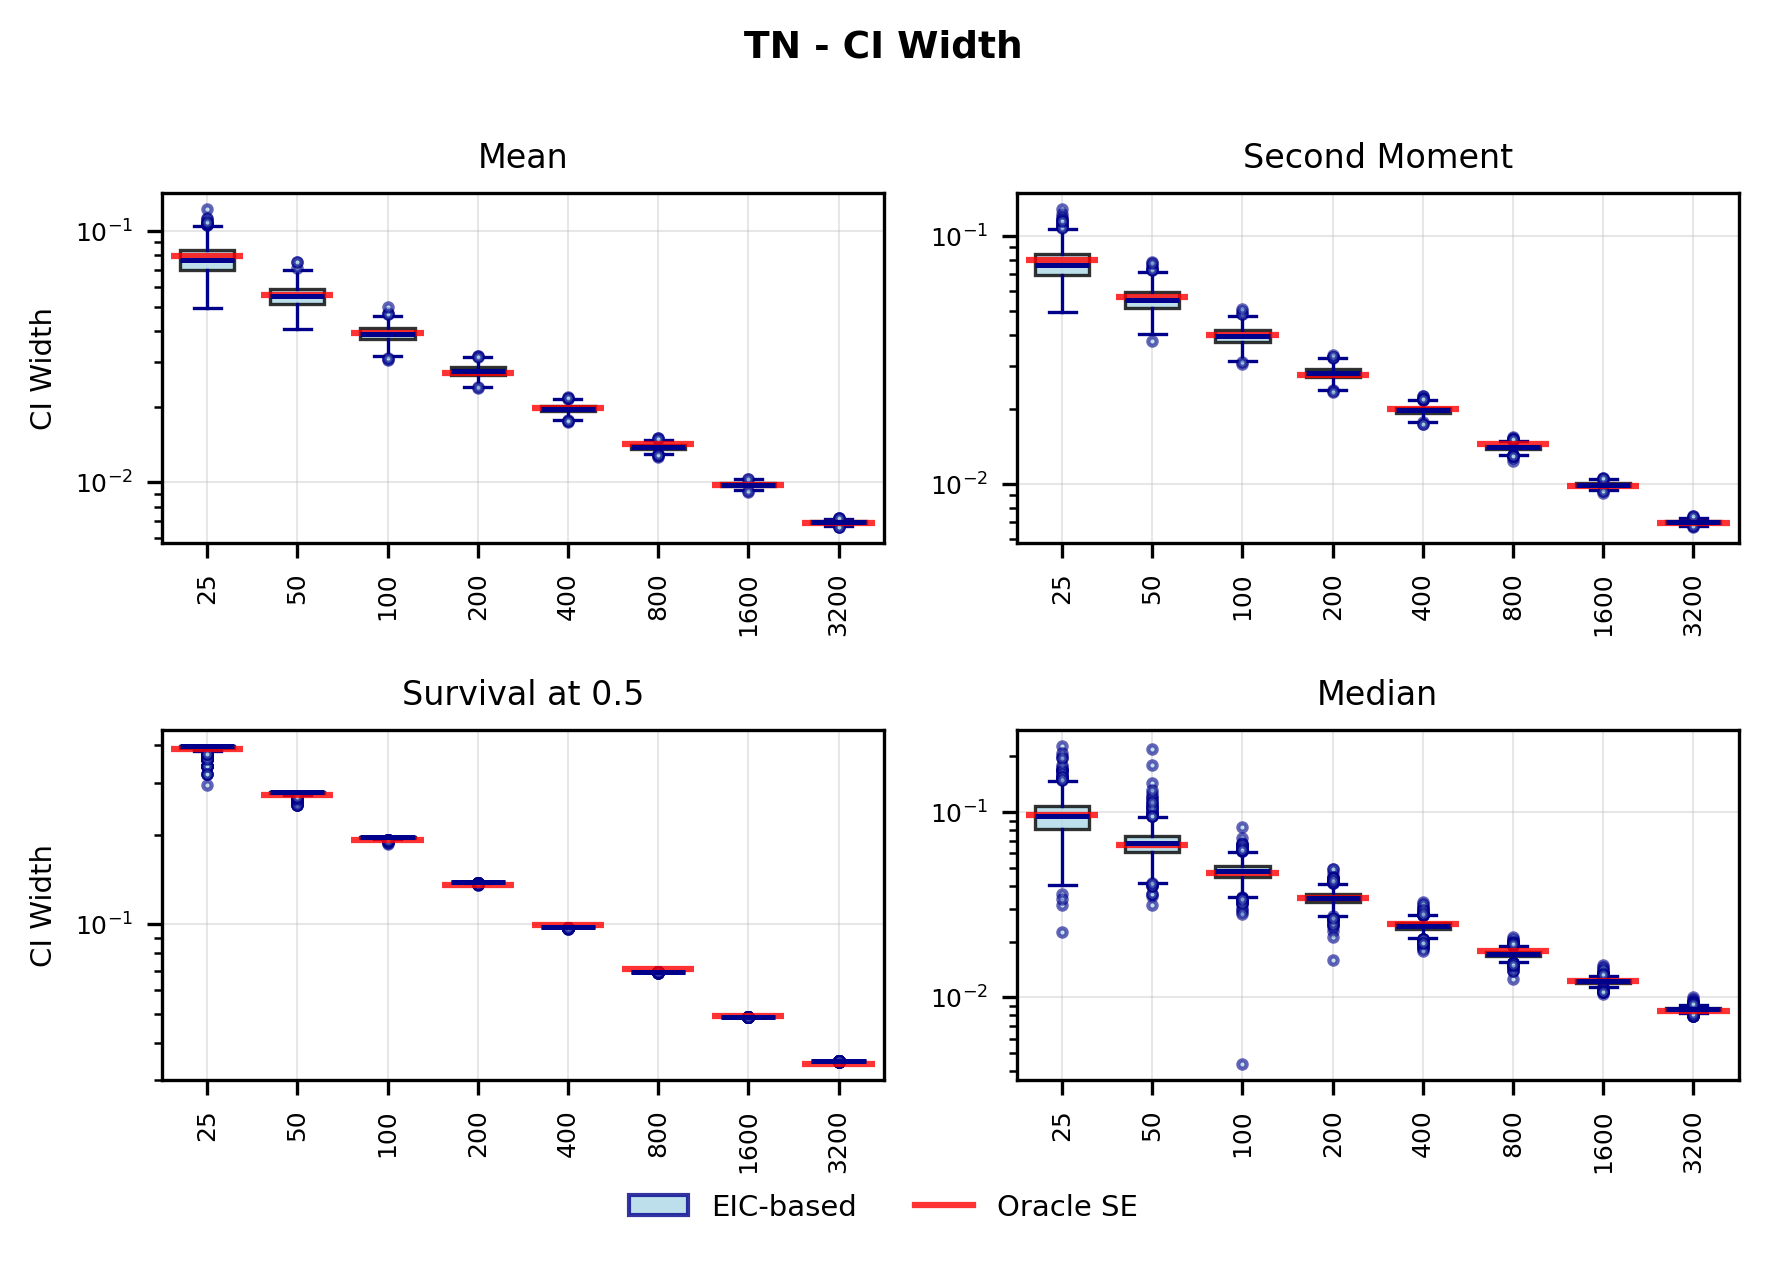
\includegraphics[width=0.75\textwidth]{resources/target_estimand_variance/Figure_CI_Width_TruncatedNormal.png}
    \caption{EIC\textendash based variance estimation for TN: CI width.}
\end{figure}

\begin{figure}[H]
    \centering
    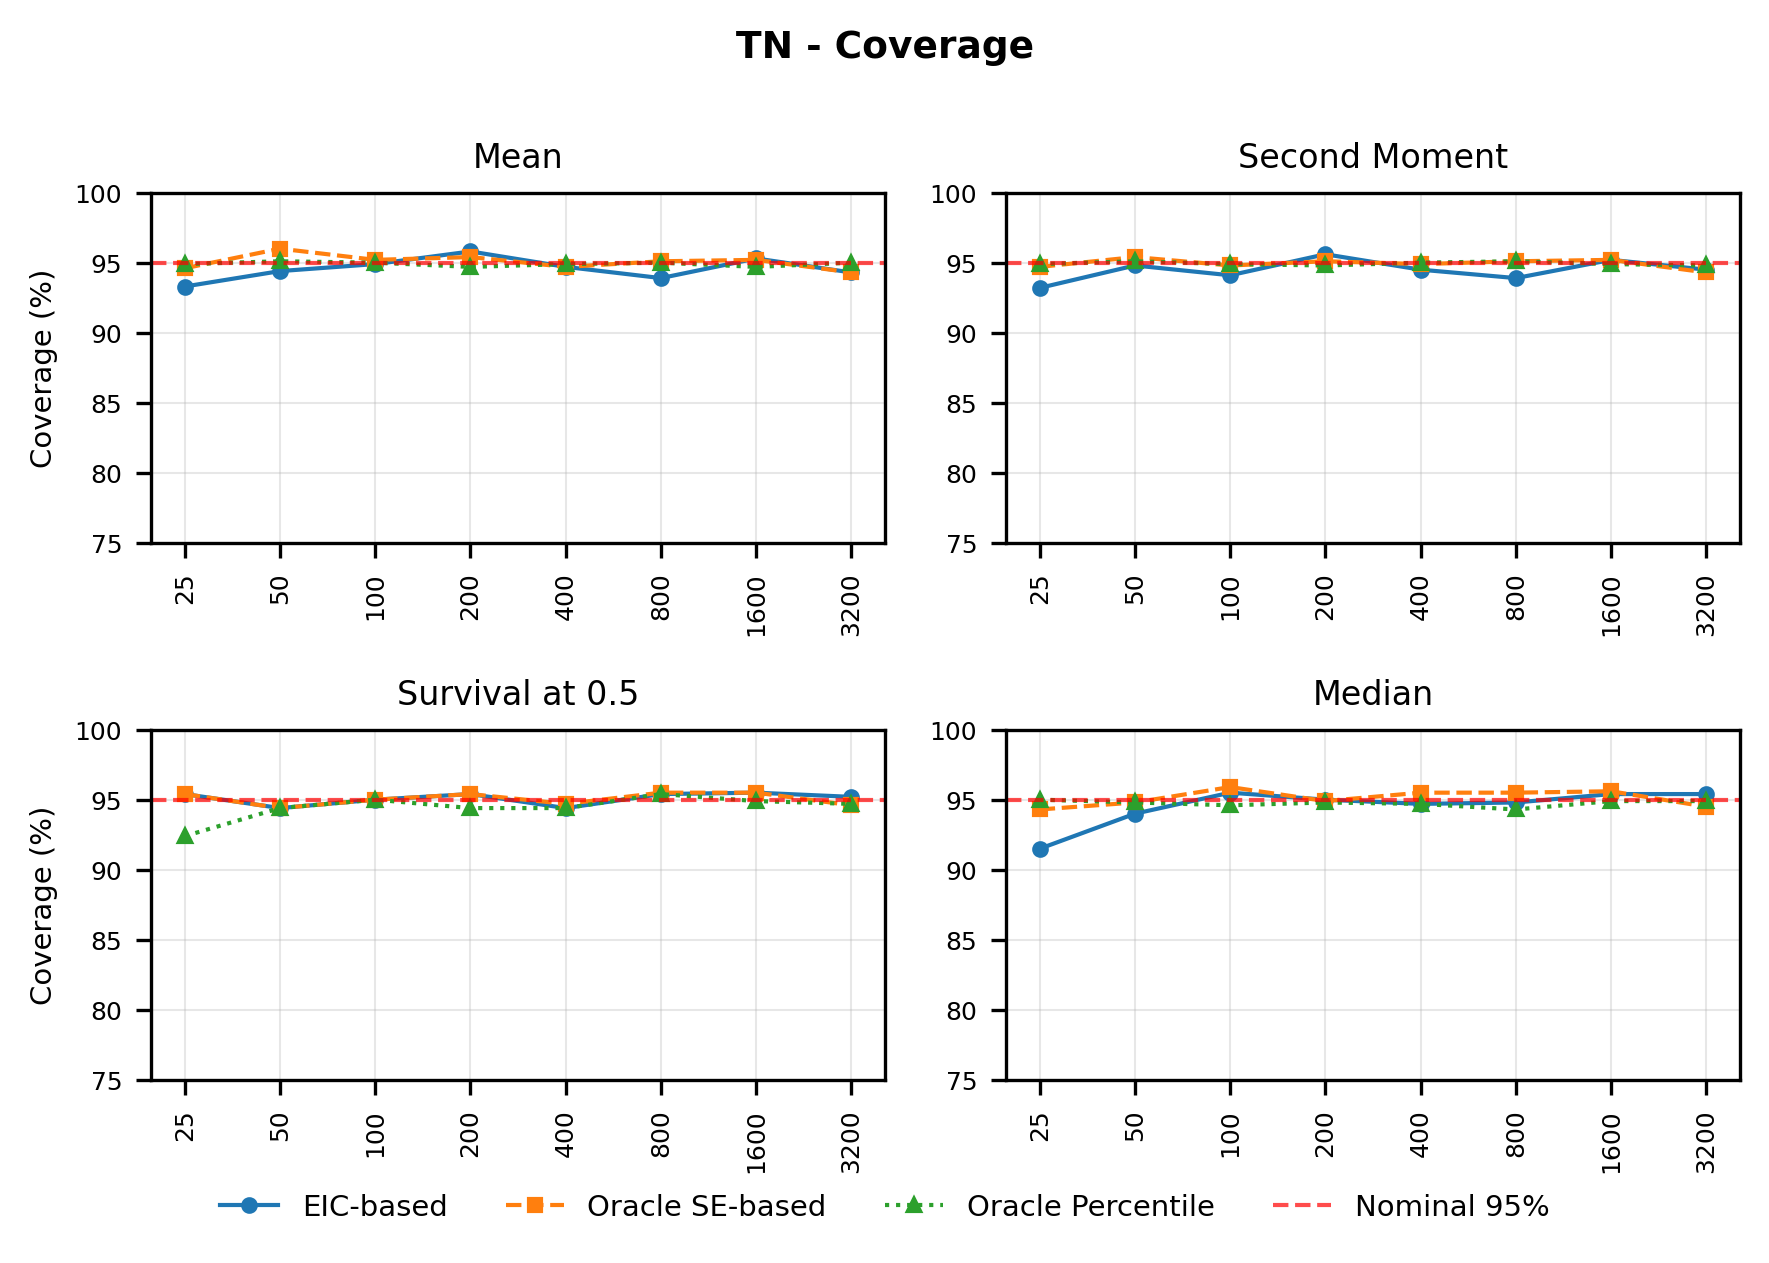
\includegraphics[width=0.75\textwidth]{resources/target_estimand_variance/Figure_Coverage_TruncatedNormal.png}
    \caption{EIC\textendash based variance estimation for TN: coverage.}
\end{figure}

\begin{figure}[H]
    \centering
    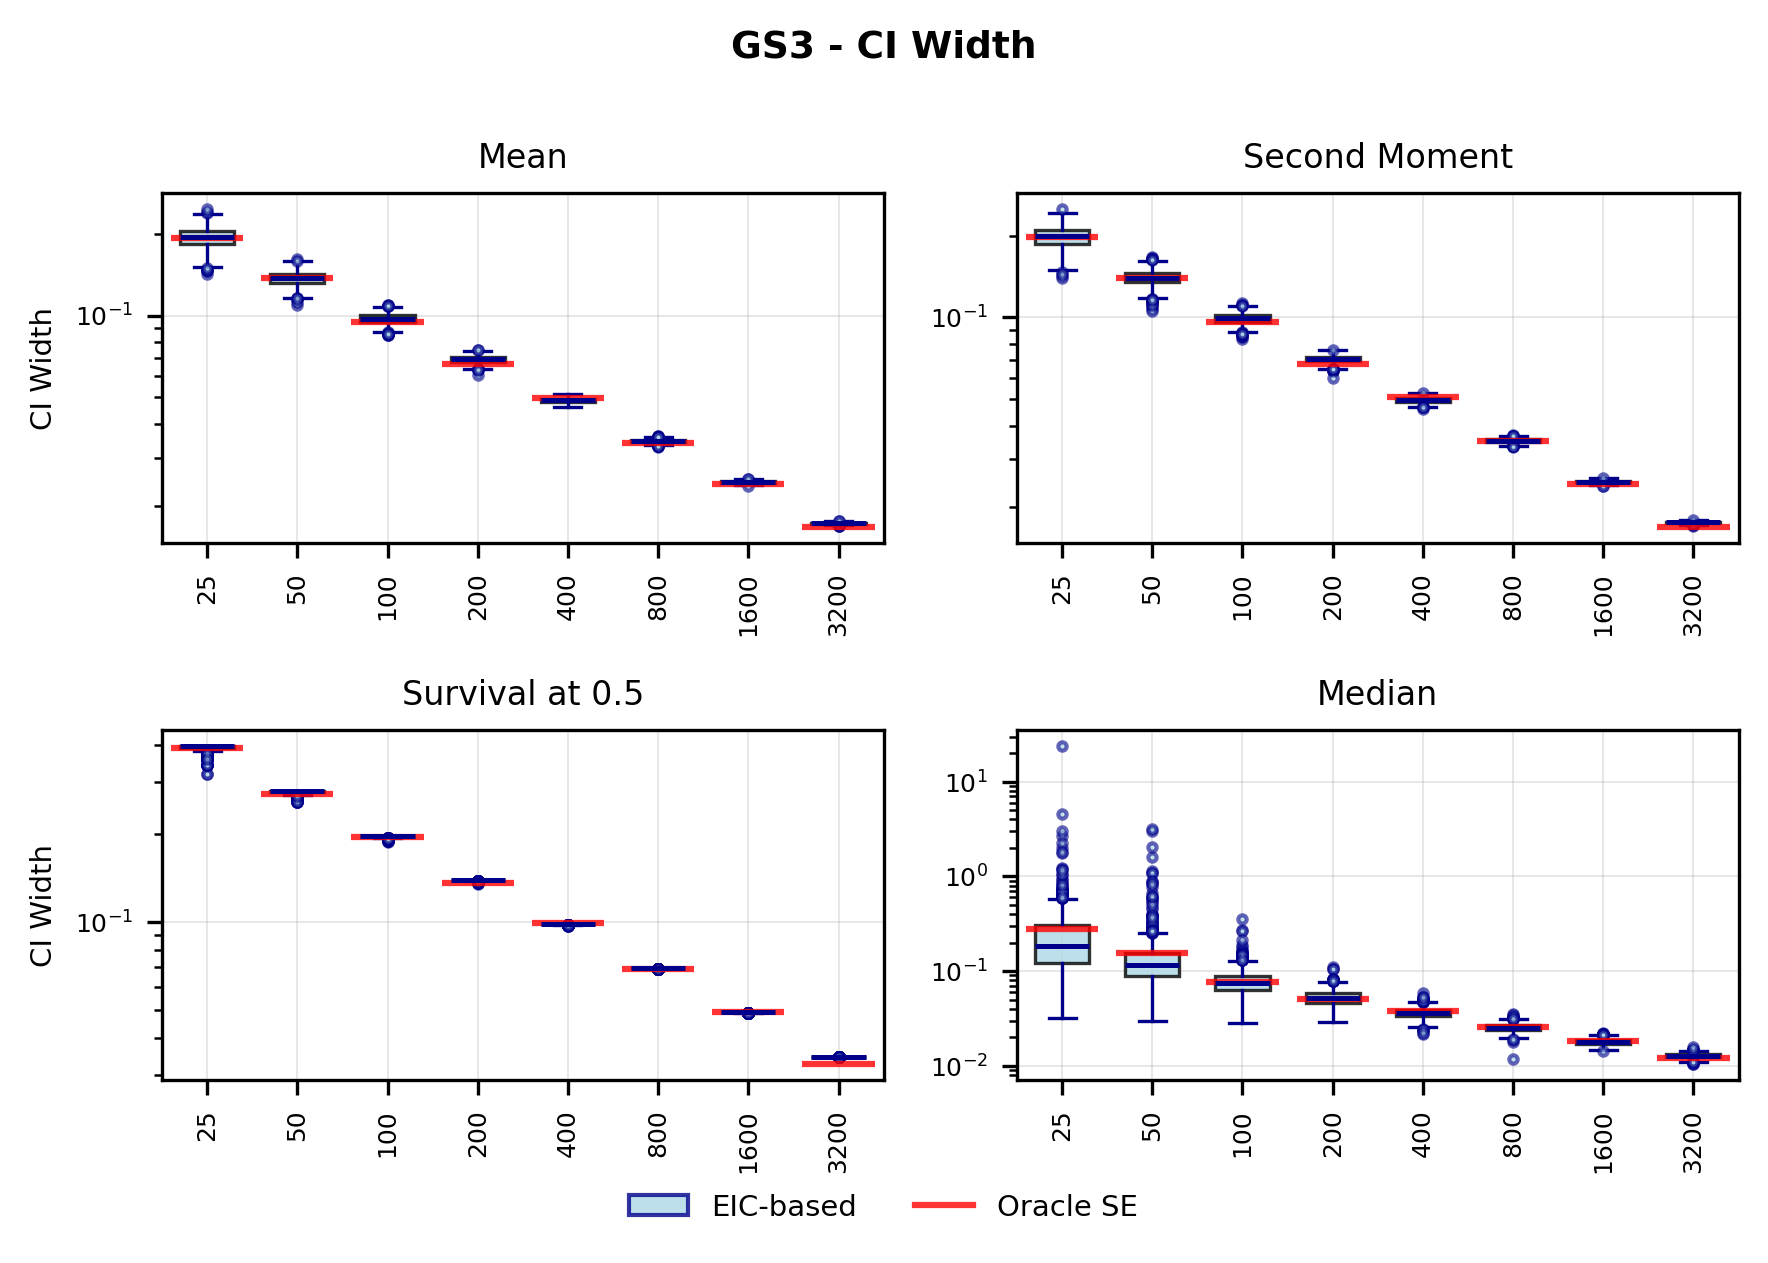
\includegraphics[width=0.75\textwidth]{resources/target_estimand_variance/Figure_CI_Width_TruncatedGMMSymmetricThree.png}
    \caption{EIC\textendash based variance estimation for GS3: CI width.}
\end{figure}

\begin{figure}[H]
    \centering
    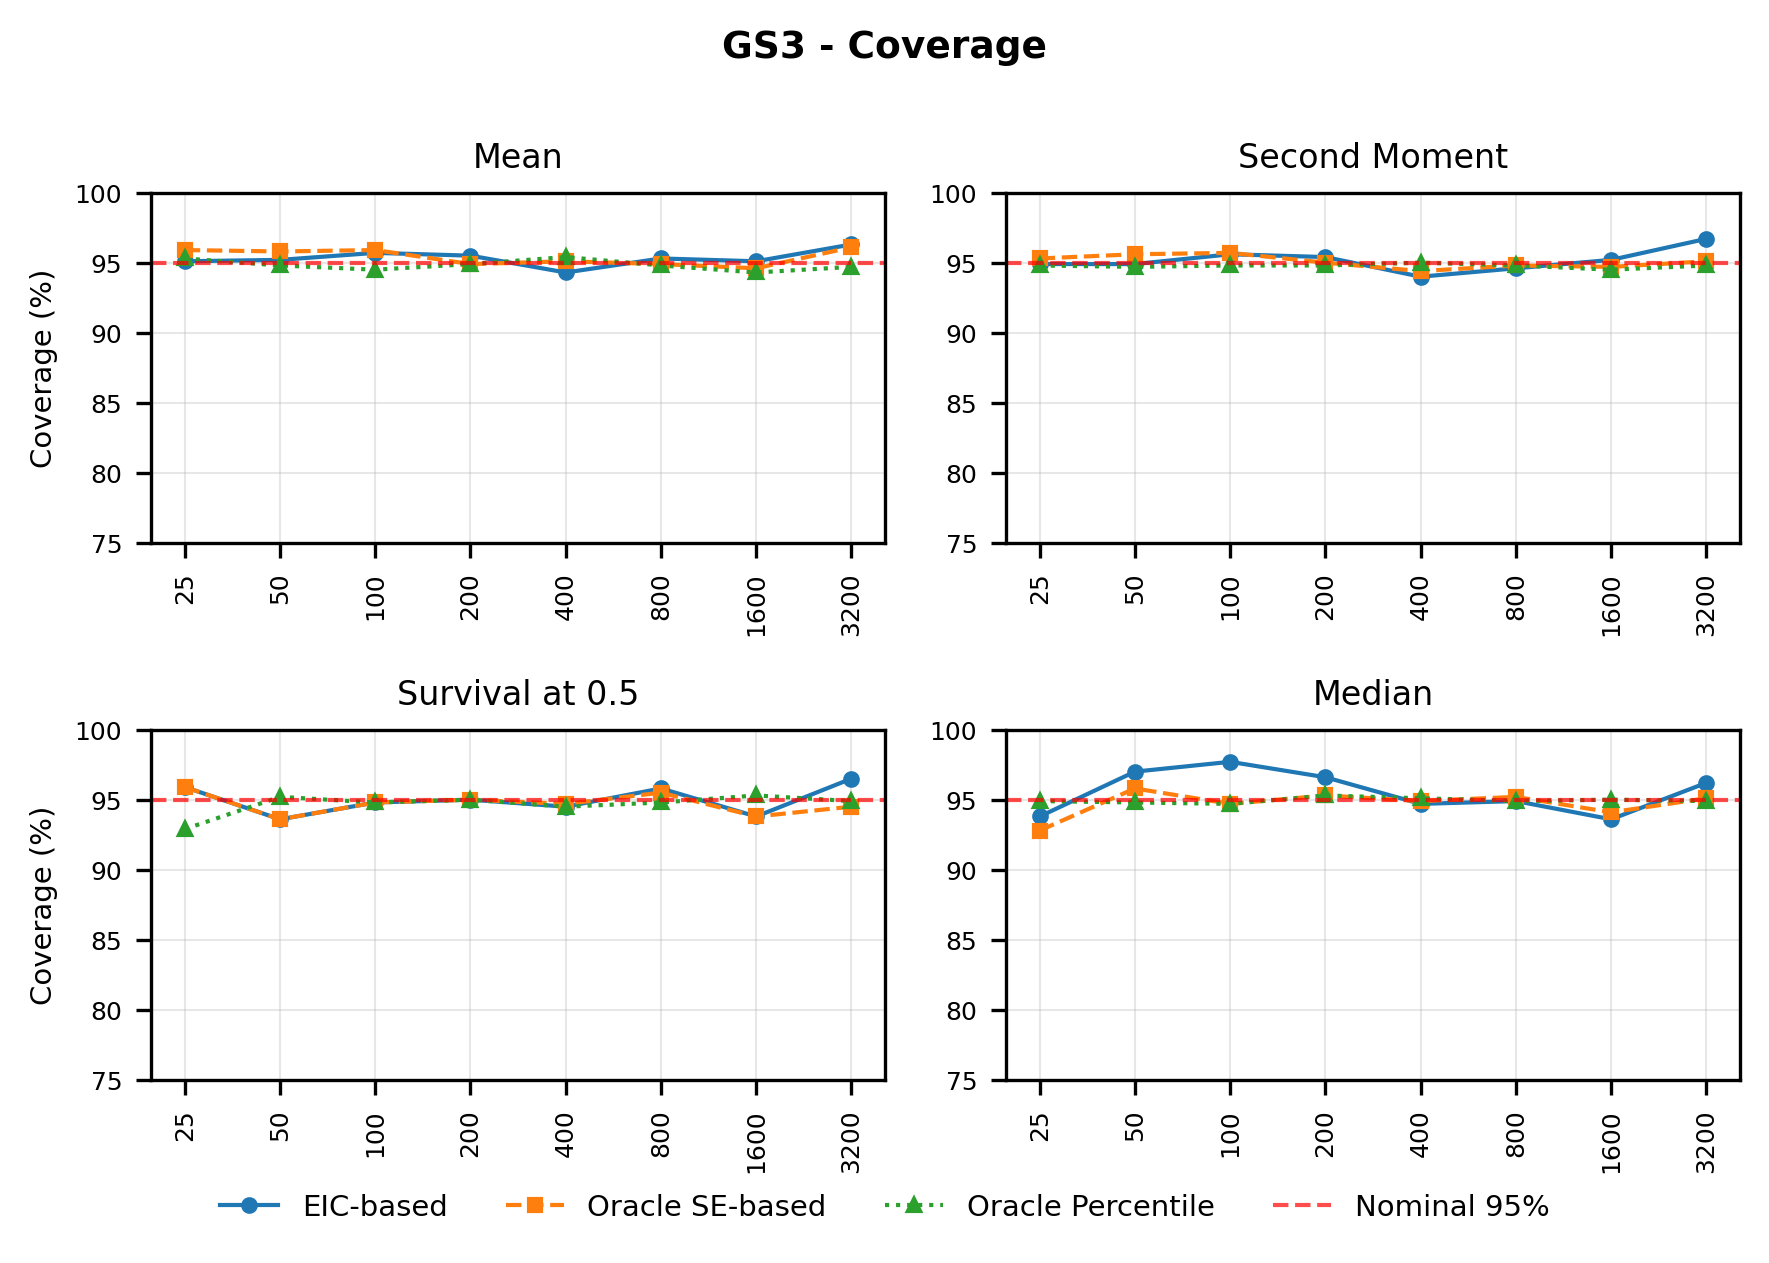
\includegraphics[width=0.75\textwidth]{resources/target_estimand_variance/Figure_Coverage_TruncatedGMMSymmetricThree.png}
    \caption{EIC\textendash based variance estimation for GS3: coverage.}
\end{figure}

\begin{figure}[H]
    \centering
    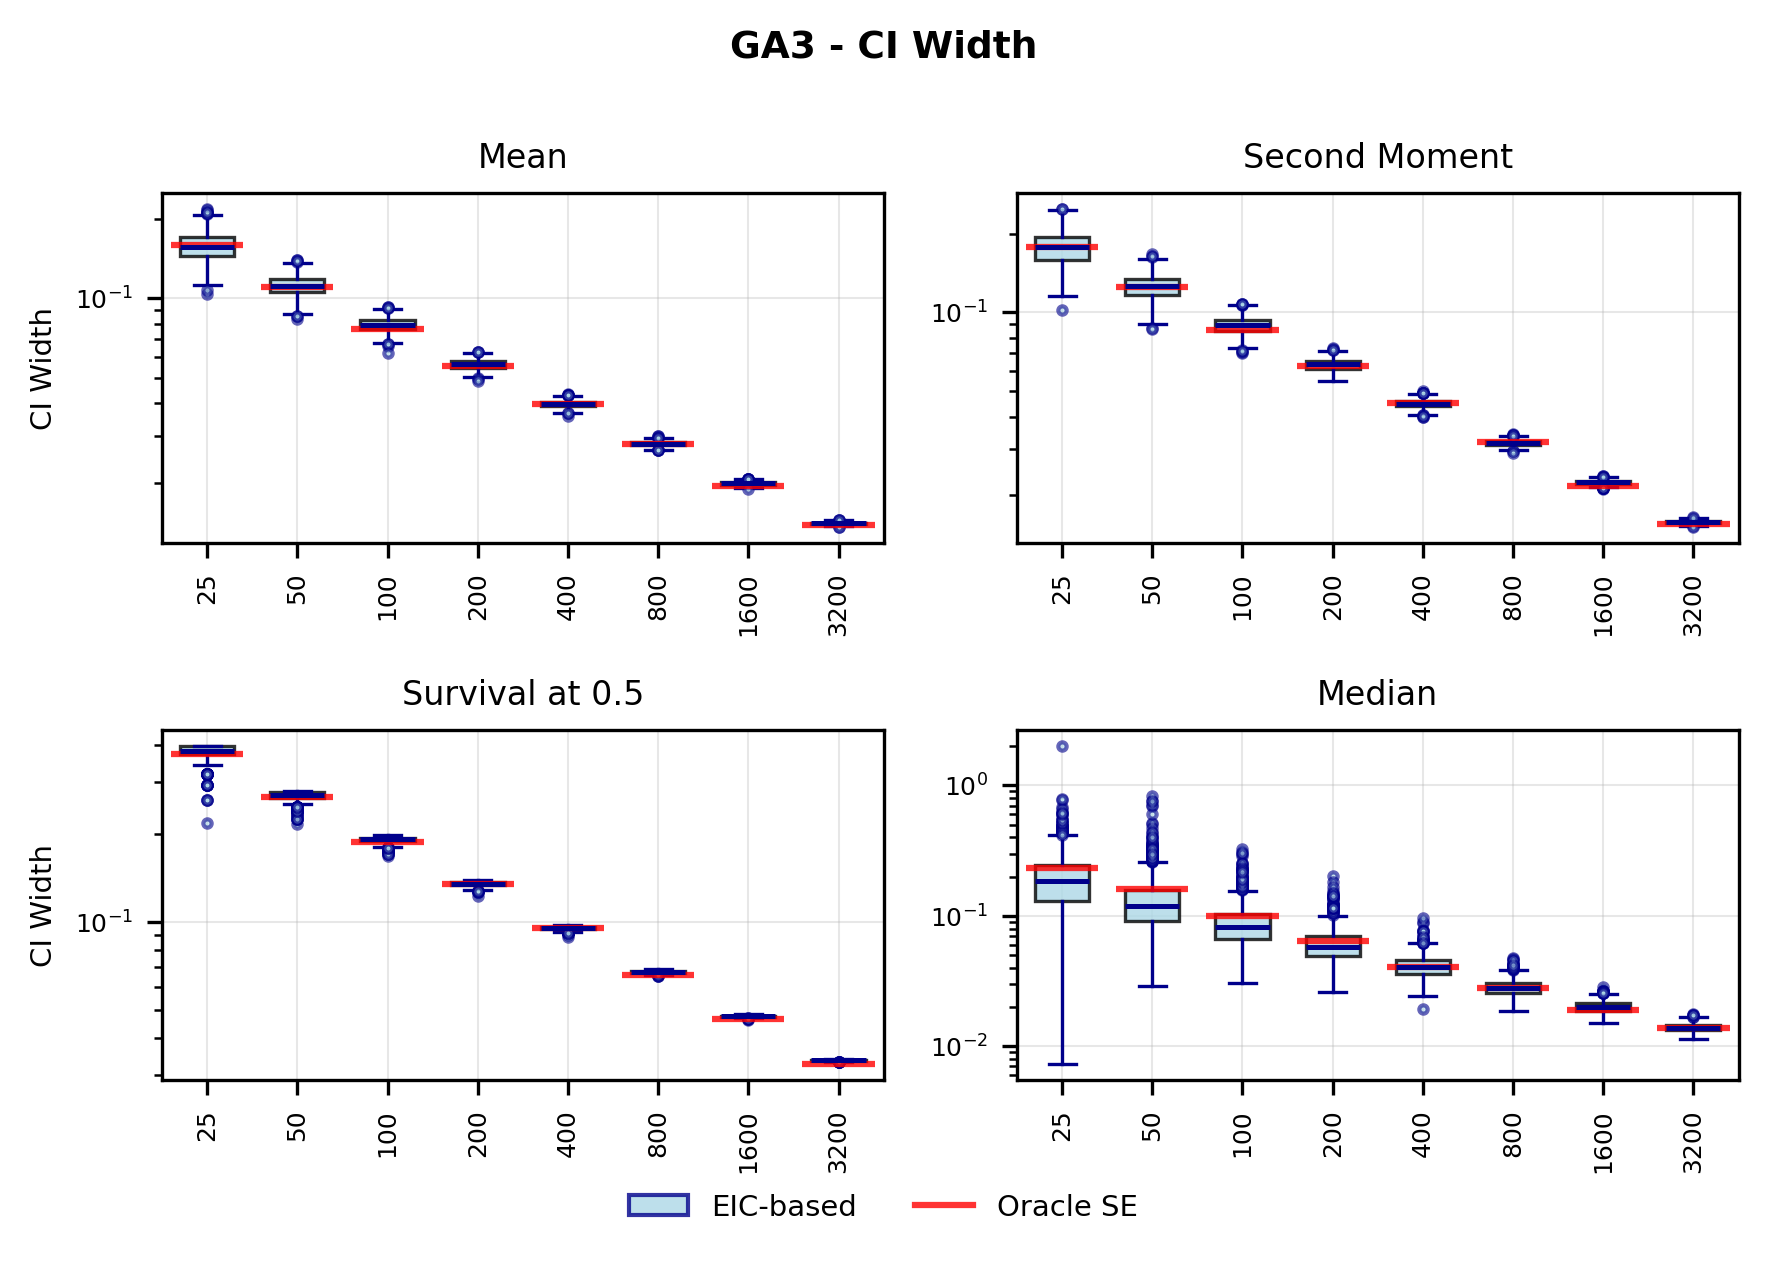
\includegraphics[width=0.75\textwidth]{resources/target_estimand_variance/Figure_CI_Width_TruncatedGMMAsymmetricThree.png}
    \caption{EIC\textendash based variance estimation for GA3: CI width.}
\end{figure}

\begin{figure}[H]
    \centering
    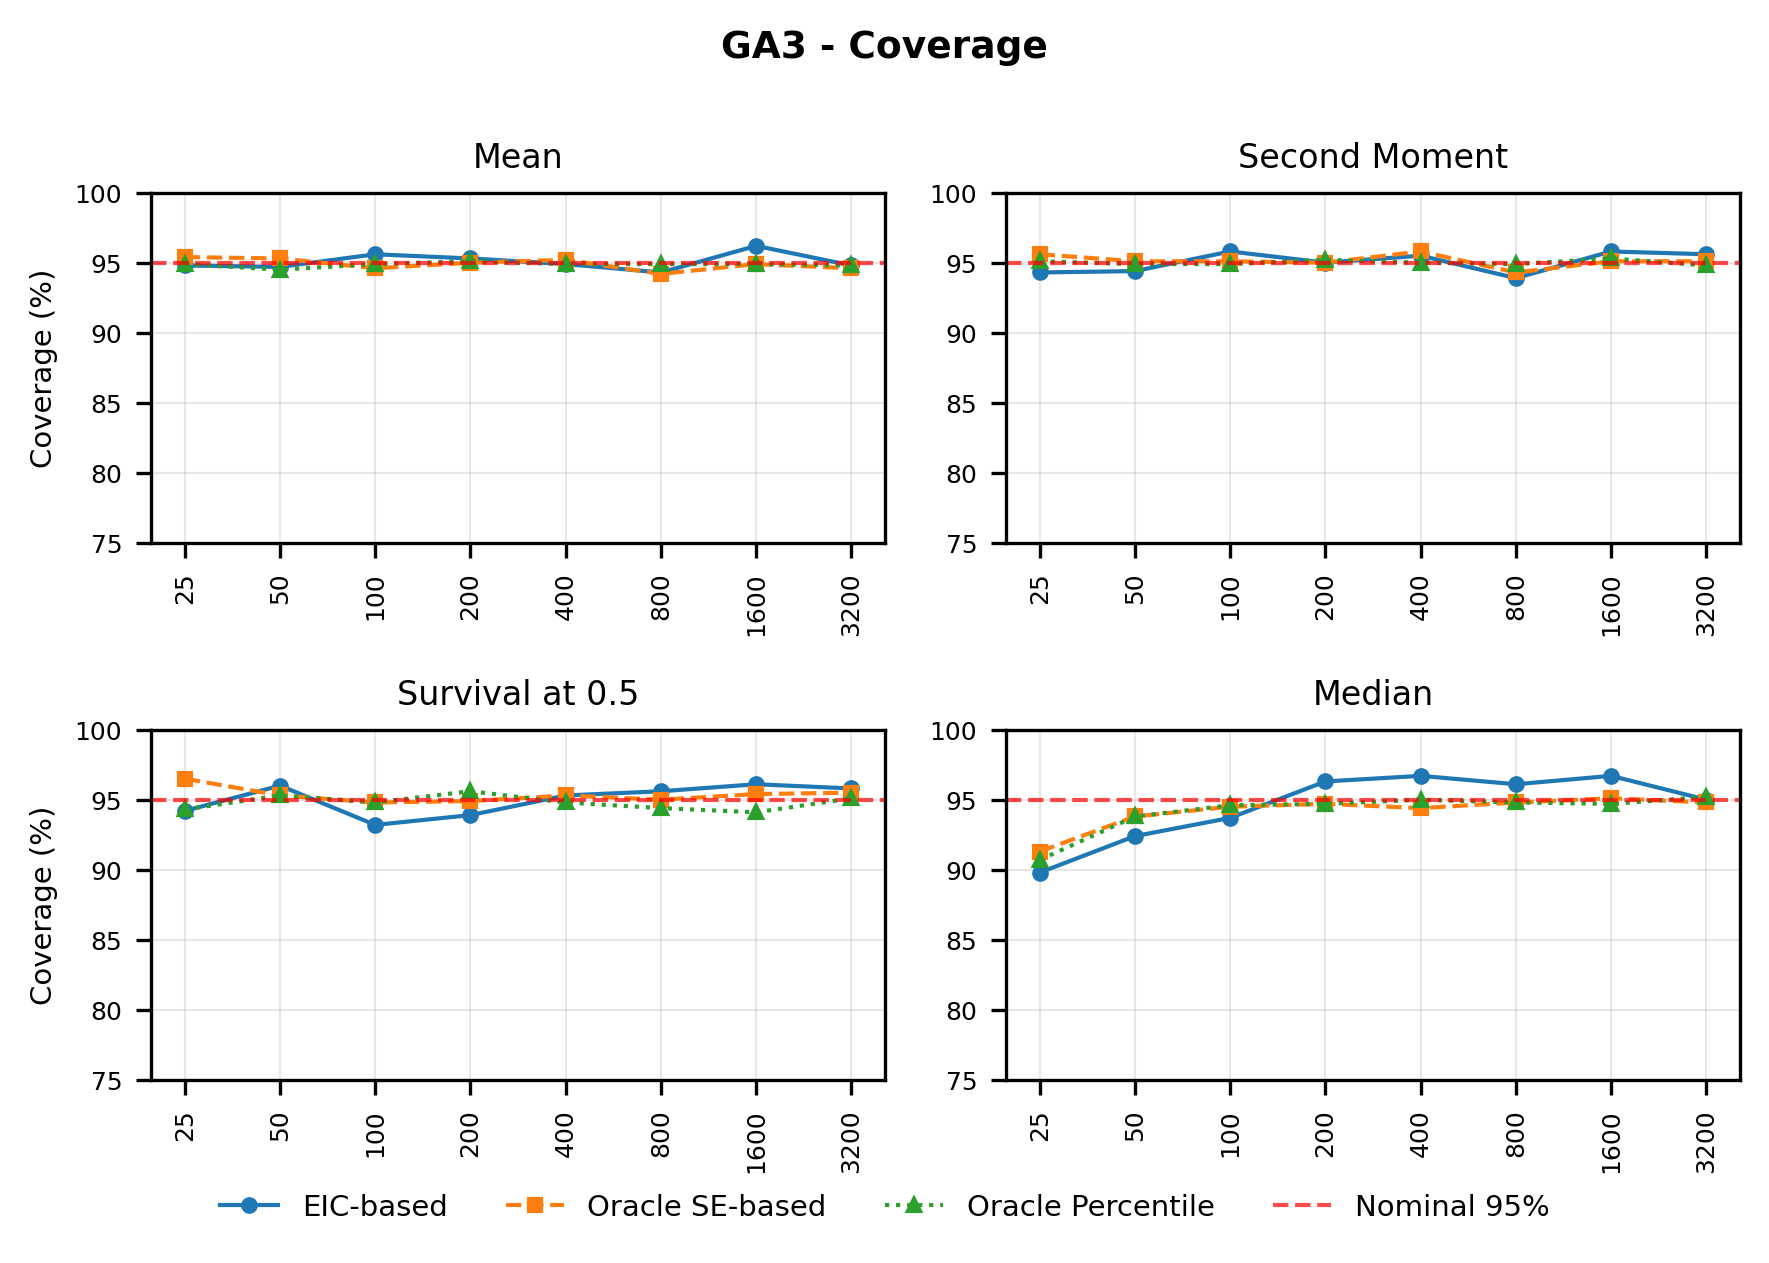
\includegraphics[width=0.75\textwidth]{resources/target_estimand_variance/Figure_Coverage_TruncatedGMMAsymmetricThree.png}
    \caption{EIC\textendash based variance estimation for GA3: coverage.}
\end{figure}

\begin{figure}[H]
    \centering
    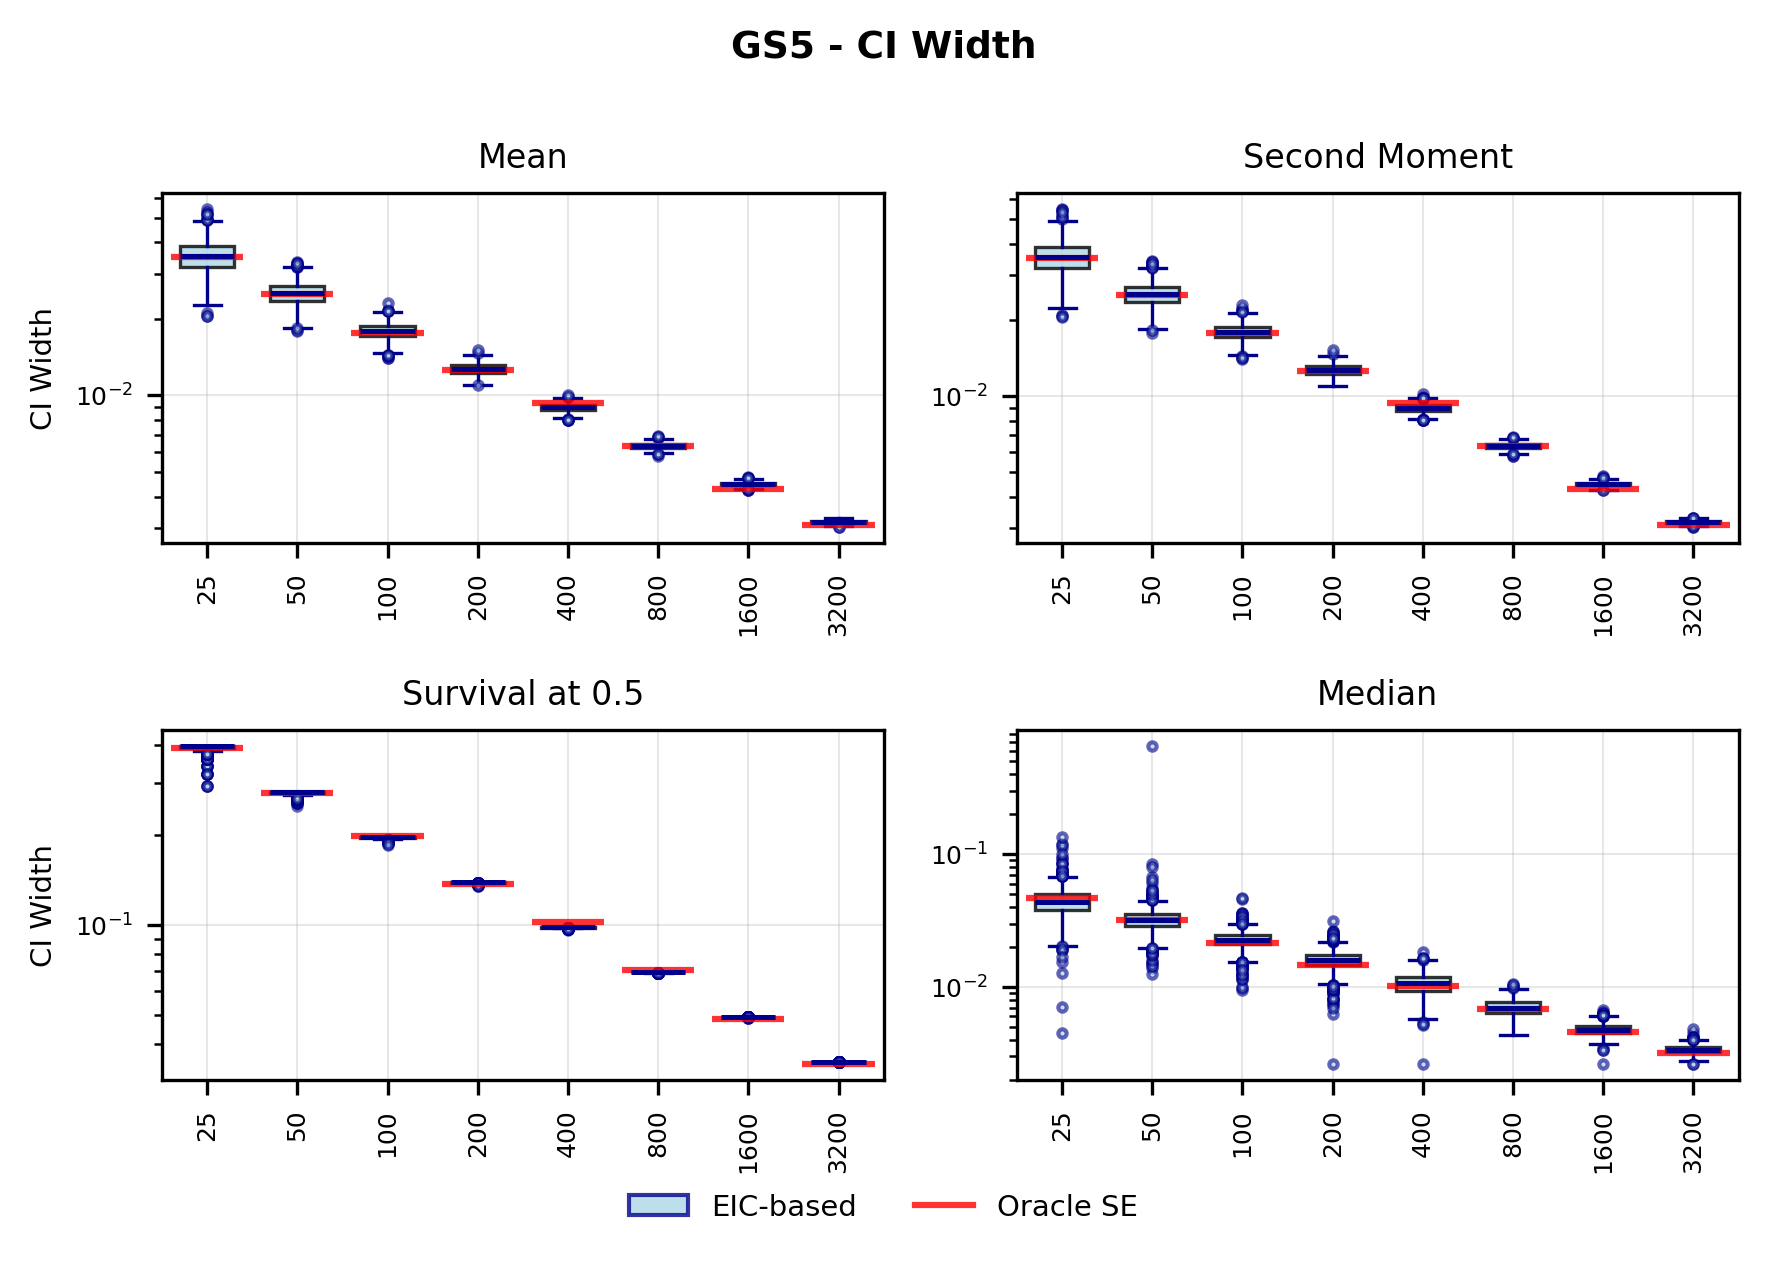
\includegraphics[width=0.75\textwidth]{resources/target_estimand_variance/Figure_CI_Width_TruncatedGMMFiveSpikes.png}
    \caption{EIC\textendash based variance estimation for GS5: CI width.}
\end{figure}

\begin{figure}[H]
    \centering
    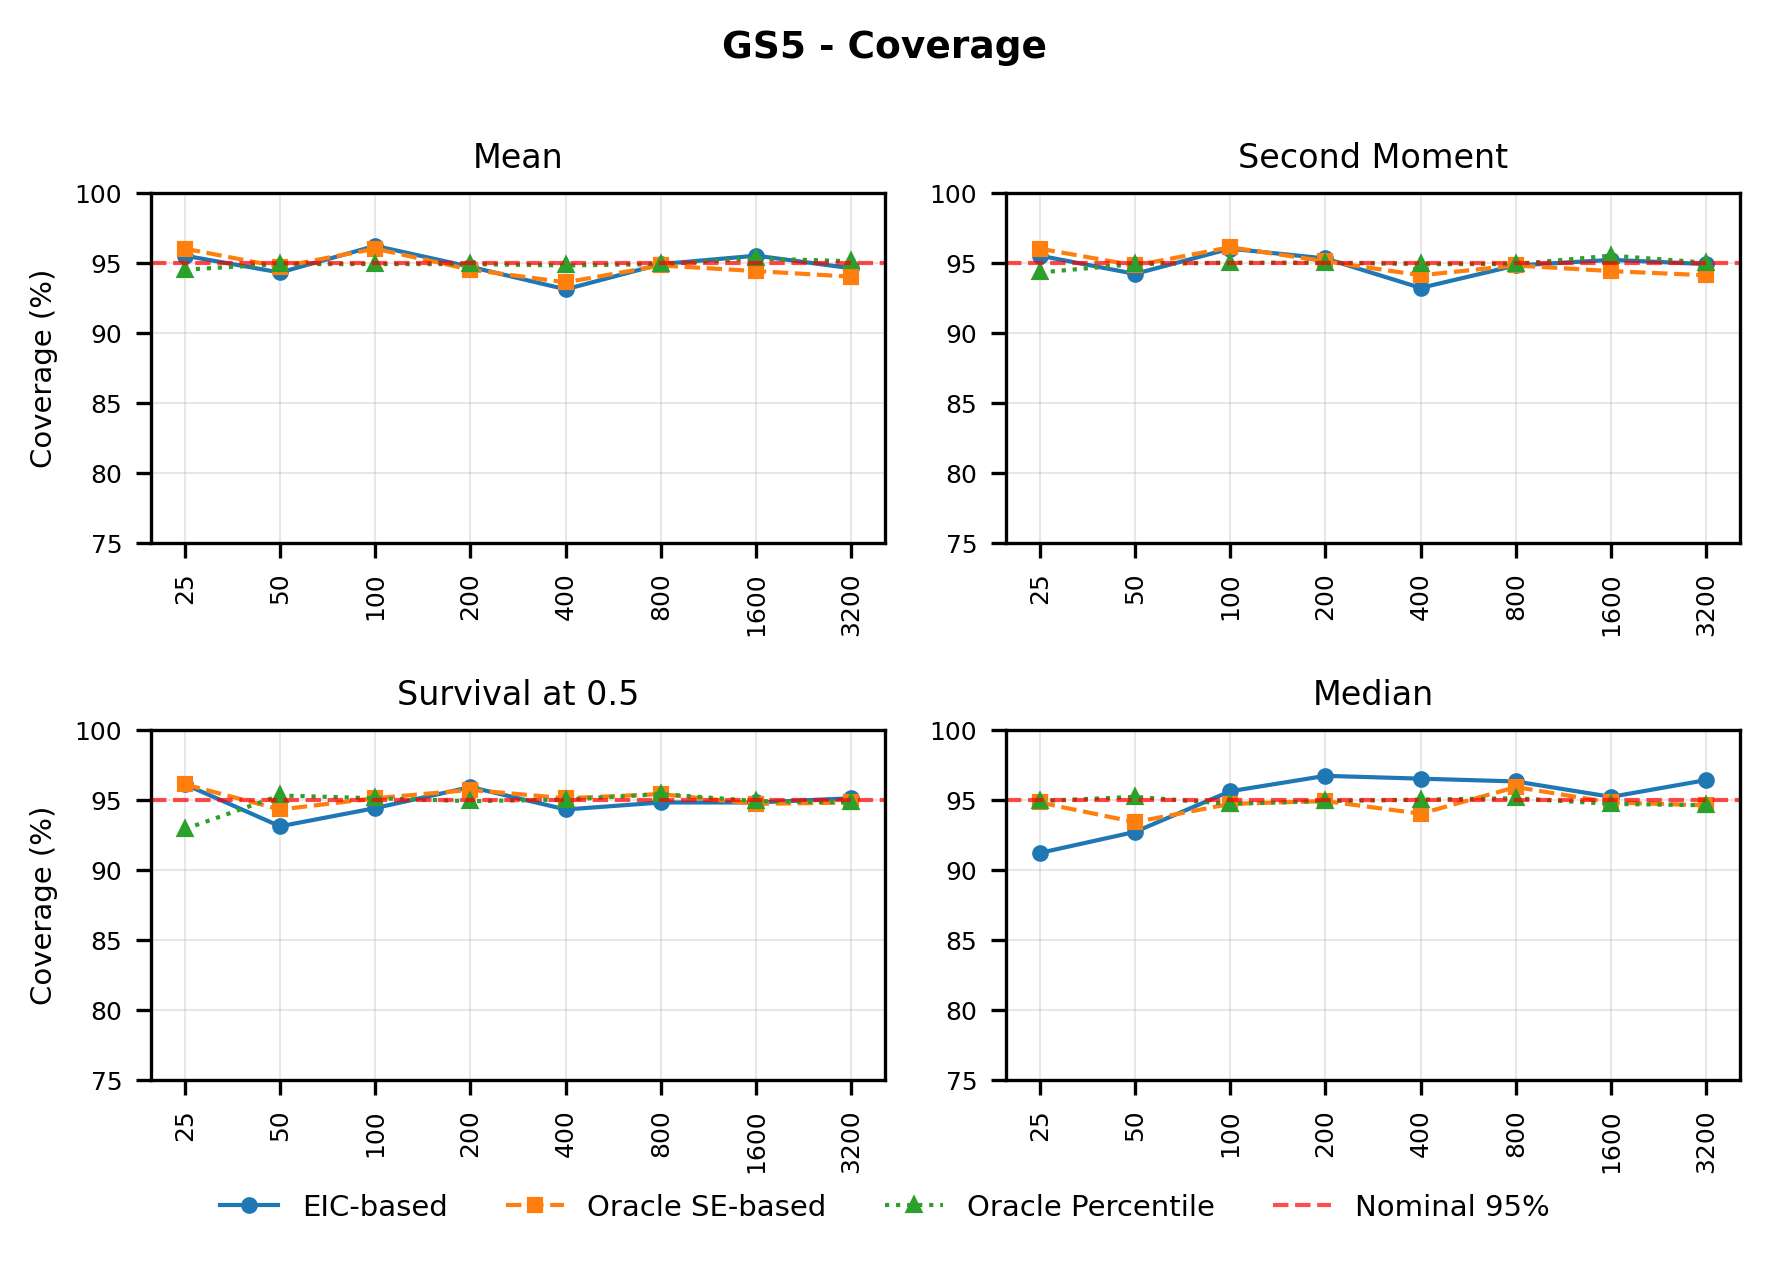
\includegraphics[width=0.75\textwidth]{resources/target_estimand_variance/Figure_Coverage_TruncatedGMMFiveSpikes.png}
    \caption{EIC\textendash based variance estimation for GS5: coverage.}
\end{figure}

\begin{figure}[H]
    \centering
    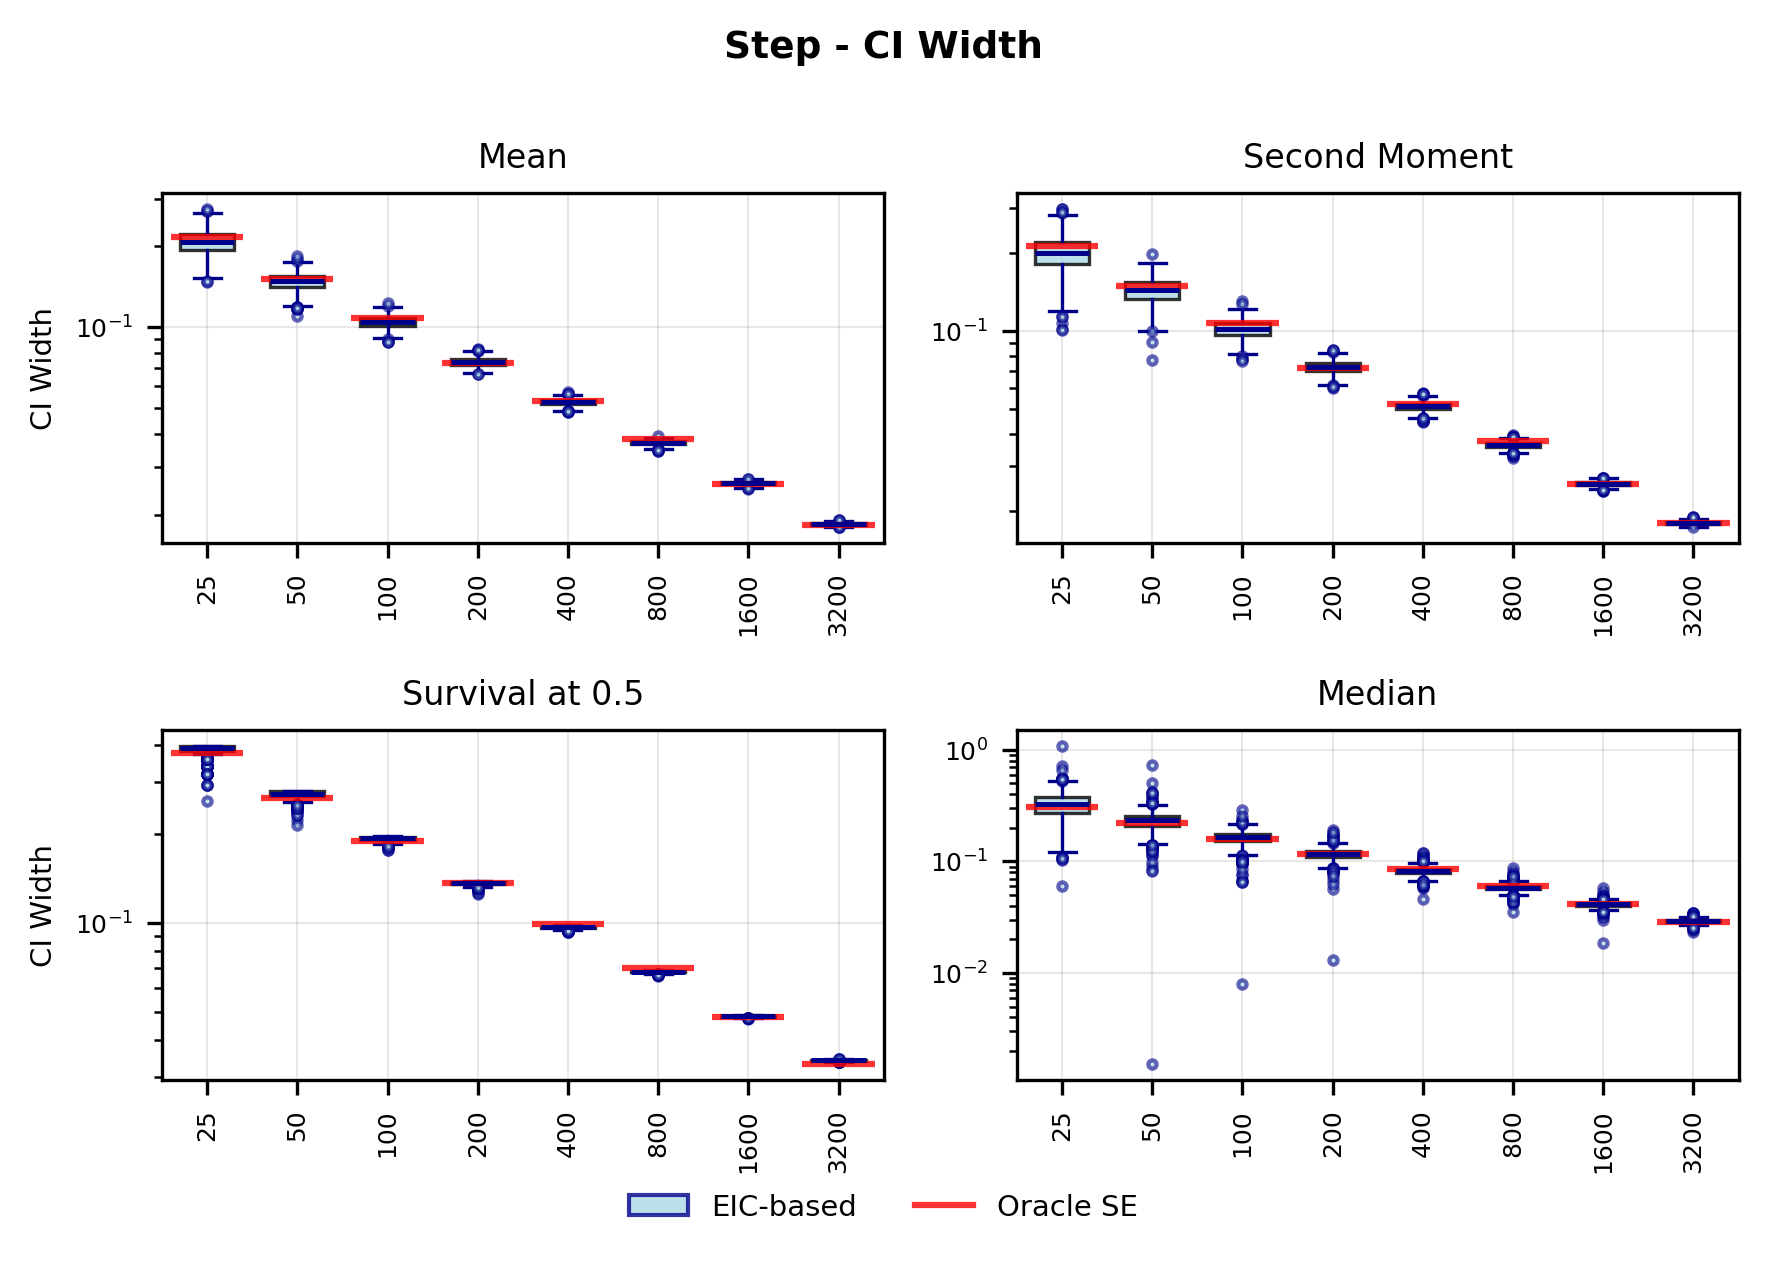
\includegraphics[width=0.75\textwidth]{resources/target_estimand_variance/Figure_CI_Width_StepFunction.png}
    \caption{EIC\textendash based variance estimation for Step: CI width.}
\end{figure}

\begin{figure}[H]
    \centering
    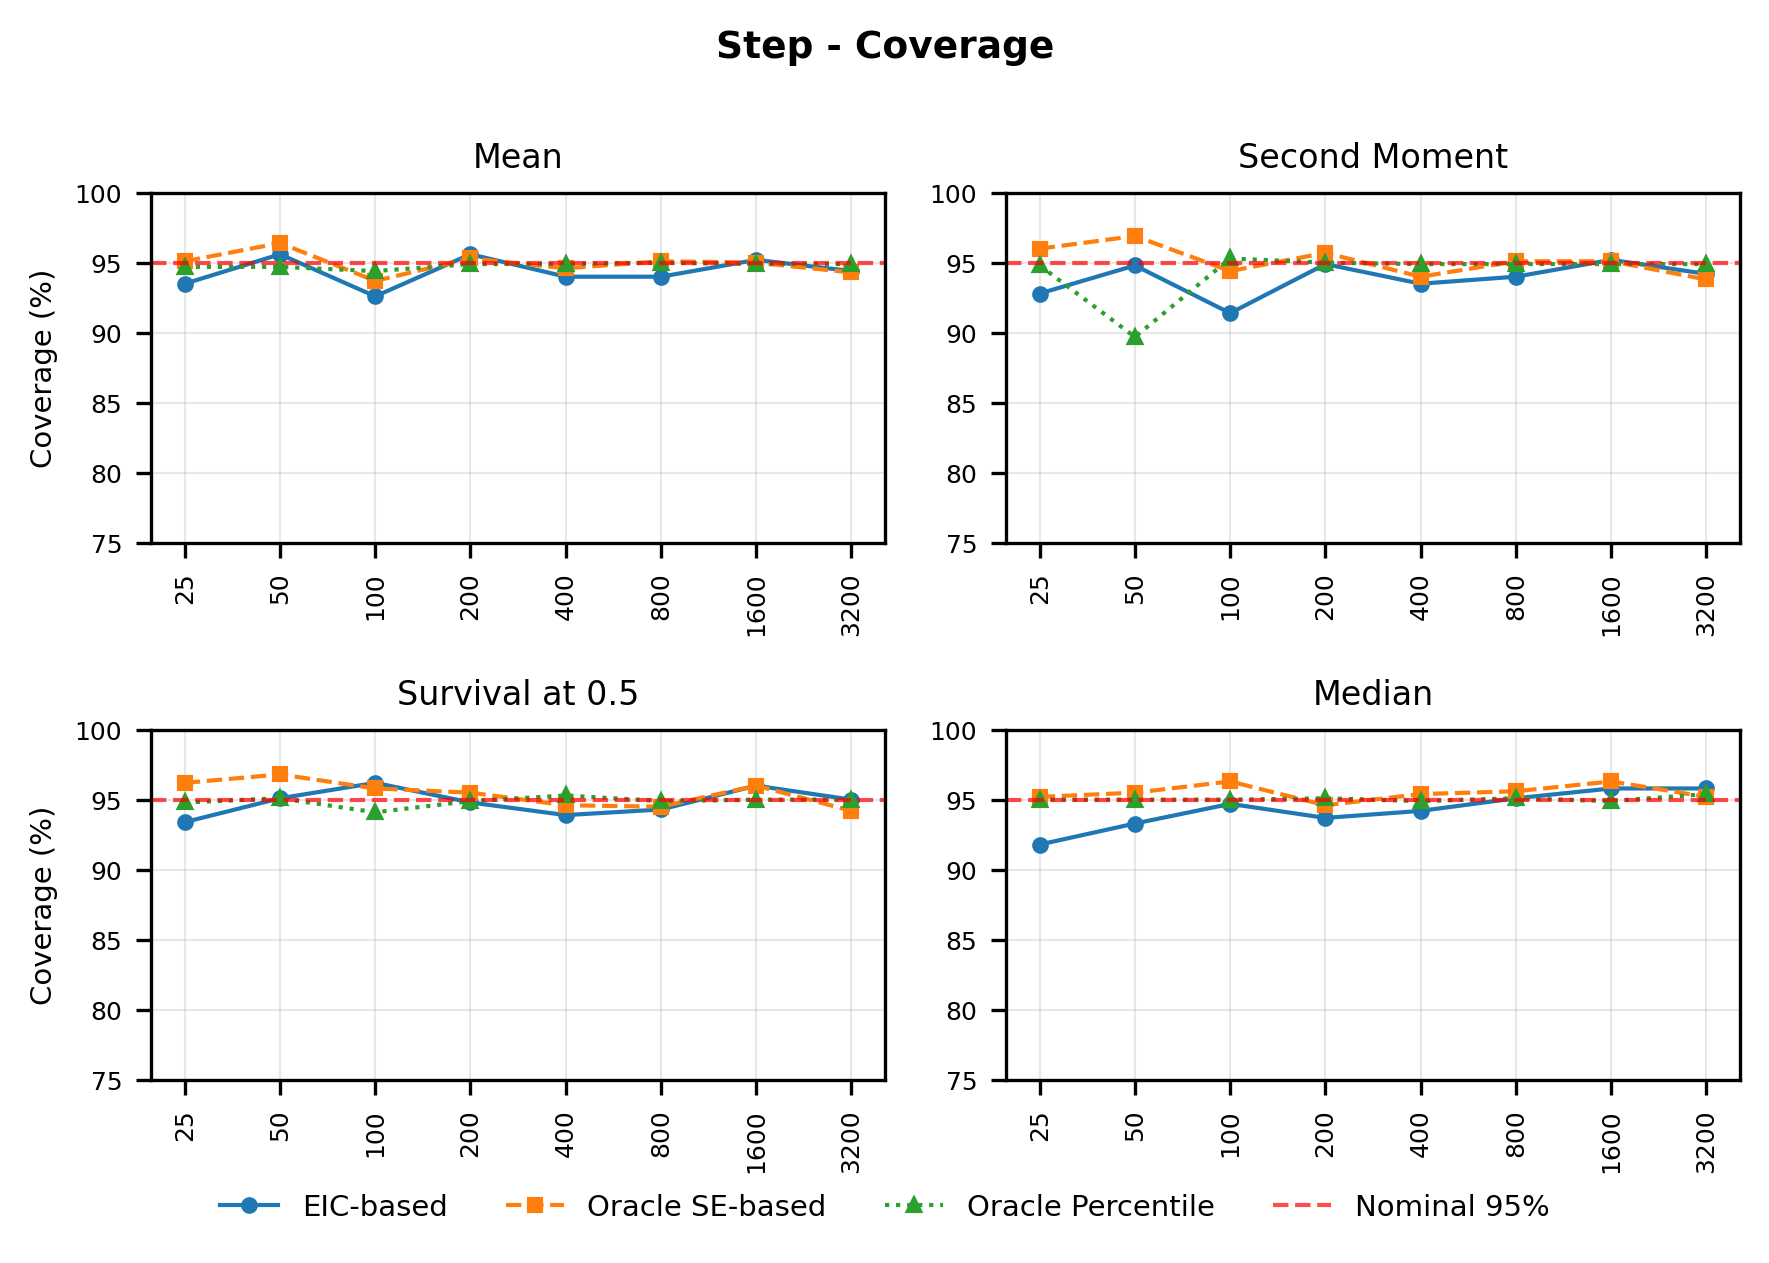
\includegraphics[width=0.75\textwidth]{resources/target_estimand_variance/Figure_Coverage_StepFunction.png}
    \caption{EIC\textendash based variance estimation for Step: coverage.}
\end{figure}

\begin{figure}[H]
    \centering
    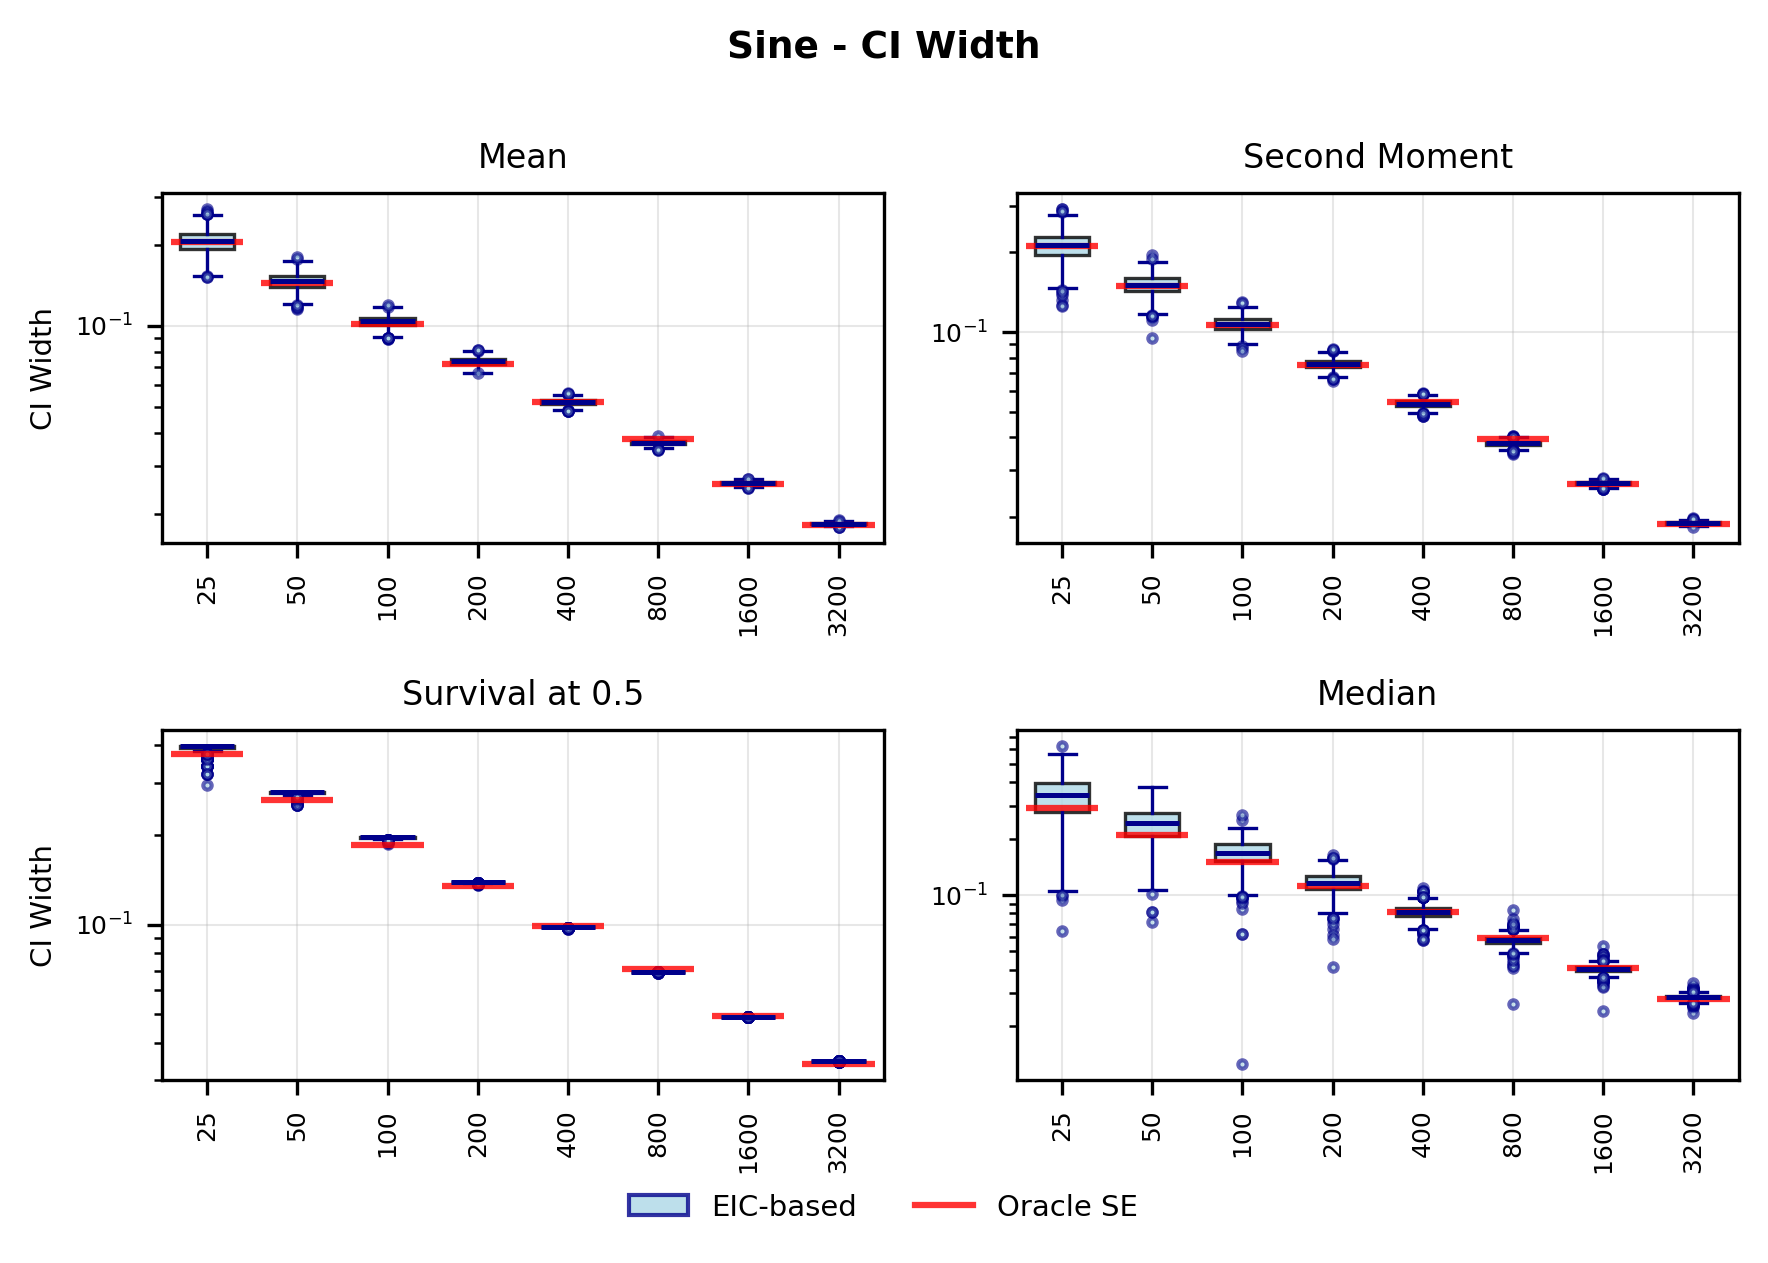
\includegraphics[width=0.75\textwidth]{resources/target_estimand_variance/Figure_CI_Width_Sinusoidal.png}
    \caption{EIC\textendash based variance estimation for Sine: CI width.}
\end{figure}

\begin{figure}[H]
    \centering
    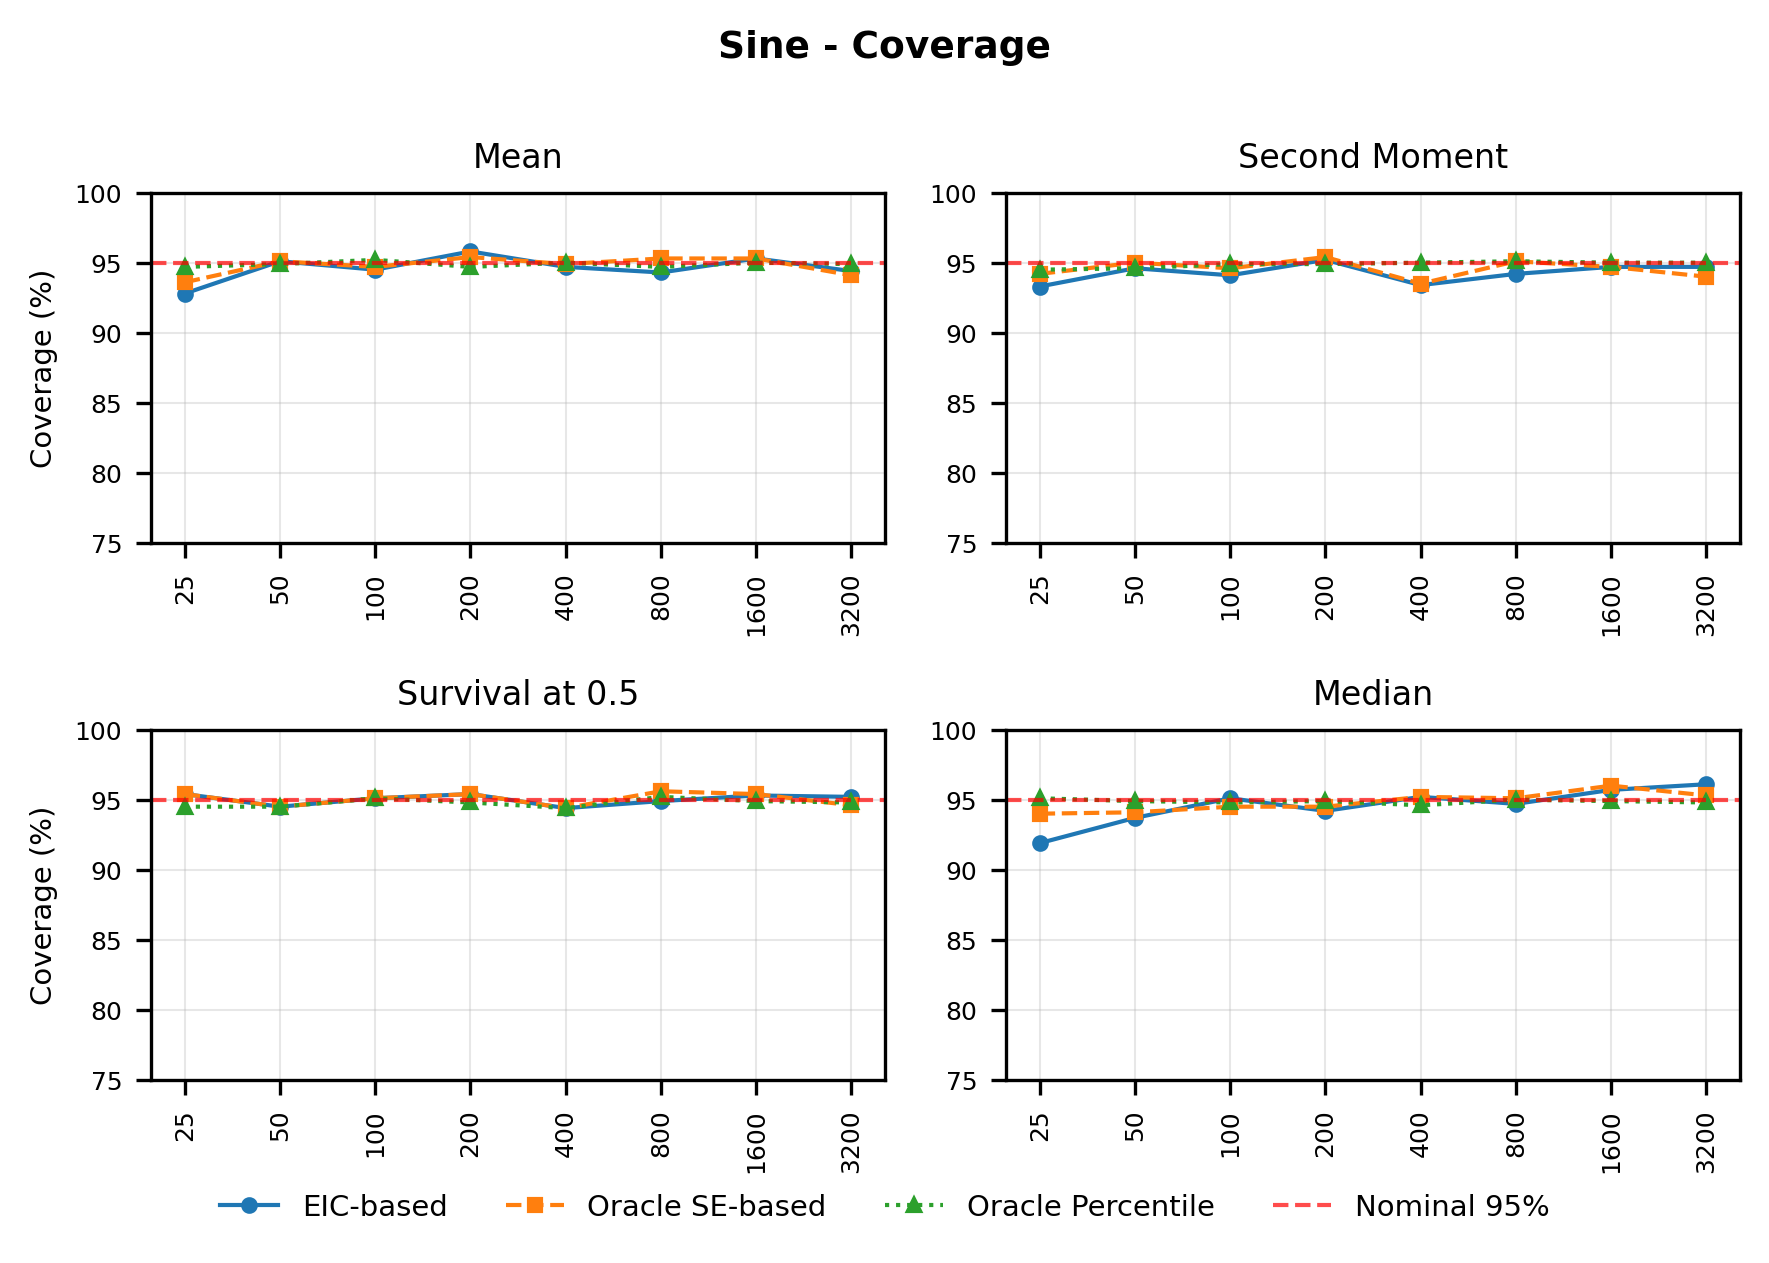
\includegraphics[width=0.75\textwidth]{resources/target_estimand_variance/Figure_Coverage_Sinusoidal.png}
    \caption{EIC\textendash based variance estimation for Sine: coverage.}
\end{figure}

\clearpage


\section{Optimization Algorithm Performance Analysis} \label{app:knot-selection}

This appendix provides comprehensive visualization of optimization algorithm performance across all six data-generating processes (DGPs) and basis orders. The figures show both knot selection behavior and loss convergence patterns for four optimization algorithms: FISTA, ProximalAdaGrad, ProximalNewton, and ProximalNewtonLBFGS, compared against the \texttt{CVXPY} reference solution.

\subsection{Notation and setup}
We denote by $n$ the number of samples, $G$ the number of midpoint intervals used for normalization on $[0,1]$, $k \in \{0,1,2\}$ the basis order, $K$ the total number of basis coefficients (intercept, $k$ polynomial terms, and $M$ truncated\,-\,power terms), $s$ the active set size used in coordinate descent, and $L_k$ the number of objective evaluations performed by backtracking at iteration $k$. Throughout, matrix\,-\,vector multiplies with dense $a\times b$ arrays are costed as $2ab$ FLOPs.

\subsection{Per-iteration FLOP derivations}
We summarize implementation\,-\,aware FLOP counts for each algorithm; see the project note \path{experiments/compare_knot_selection/algorithm_flop_per_iter.md} in the experiment git repo for additional commentary and logging details.

\paragraph{FISTA} A forward pass on data and midpoints and a backward pass via autograd each cost $\Theta\big((n+G)K\big)$, with an additional $\Theta(GK)$ for the exact normalization update. Dominant term: $\Theta\big((n+G)K\big)$.

\paragraph{Proximal AdaGrad} Computing the gradient uses $\Theta\big(nK + GK\big)$; forming the diagonal Hessian via variance on midpoints contributes another $\Theta(GK)$ (tighter bound) to $\Theta(3GK)$ (conservative). Including the normalization step yields a dominant $\Theta\big((n+G)K\big)$.

\paragraph{Proximal Newton (full)} Each iteration forms the gradient in $\Theta\big((n+G)K\big)$, the Hessian as a weighted covariance on midpoints in $\Theta\big(GK^2\big)$, solves the proximal subproblem via coordinate descent in $\Theta\big(sK^2\big)$, and performs $L_k$ objective evaluations contributing $\Theta\big(L_k (n+G)K\big)$; normalization adds $\Theta(GK)$. Dominant term: $\Theta\big(GK^2 + sK^2\big) + \Theta\big((1+L_k)(n+G)K\big)$.

\paragraph{Proximal Newton L\,-\,BFGS} Replacing the full Hessian with an L\,-\,BFGS update avoids the $GK^2$ term; per iteration is dominated by the gradient and line search plus normalization: $\Theta\big((1+L_k)(n+G)K\big)$.

\subsection{From iterations to cumulative FLOPs}
Given per\,-\,iteration FLOP estimates $F(k)$, cumulative FLOPs up to iteration $t$ are $C(t) = \sum_{k=1}^t F(k)$. Our visualization utilities infer $L_k$ from logged step sizes $\alpha_k$ (with backtracking factor $\beta=0.5$) and use consistent baselines at iteration/FLOP zero. See the note for practical defaults and alignment details.

\begin{figure}[H]
    \centering
    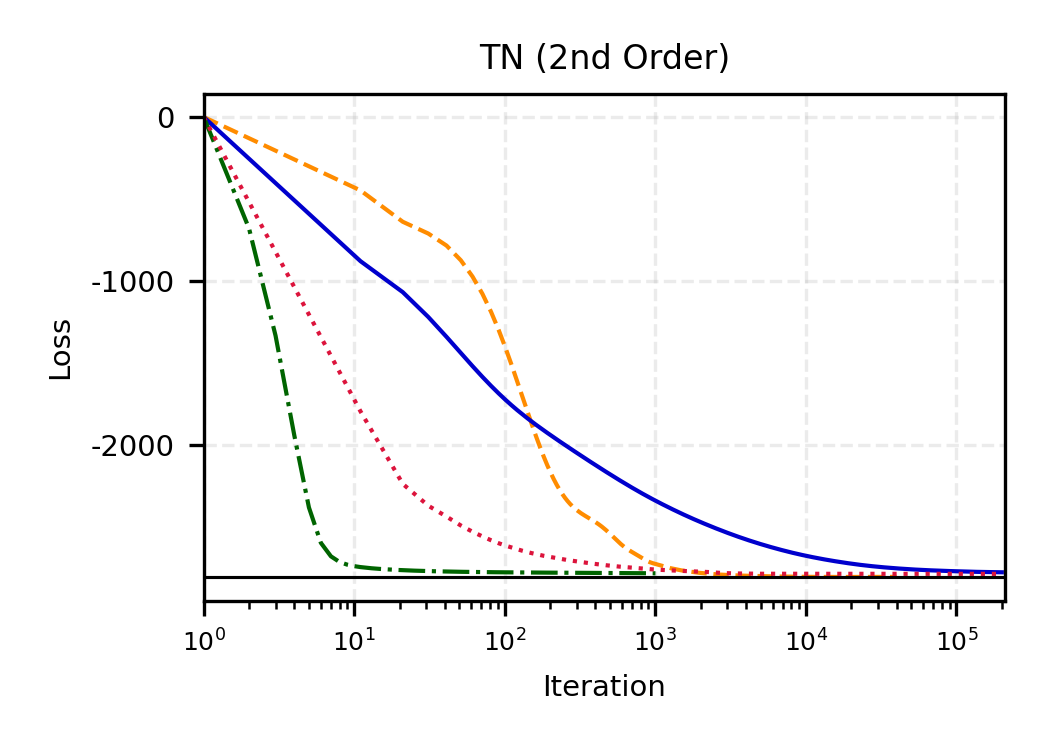
\includegraphics[width=.49\textwidth]{resources/optimization_algorithms/per_iter/TruncatedNormal_order_2_loss_per_iter.png}
    \hfill
    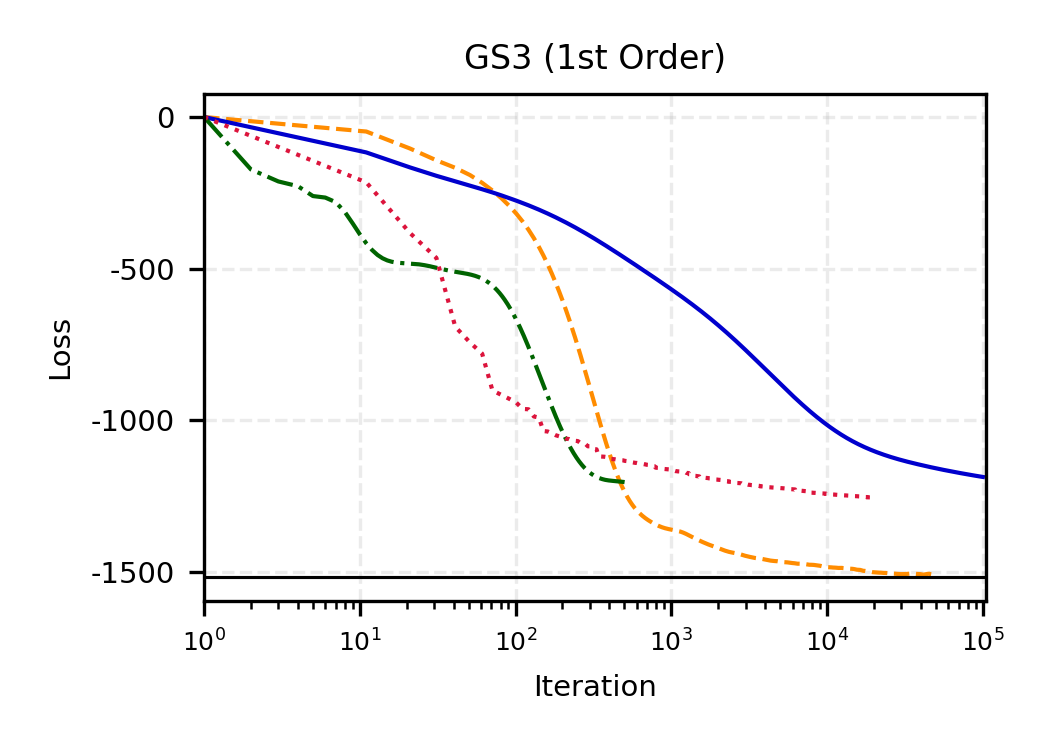
\includegraphics[width=.49\textwidth]{resources/optimization_algorithms/per_iter/TruncatedGMMSymmetricThree_order_1_loss_per_iter.png}
    
    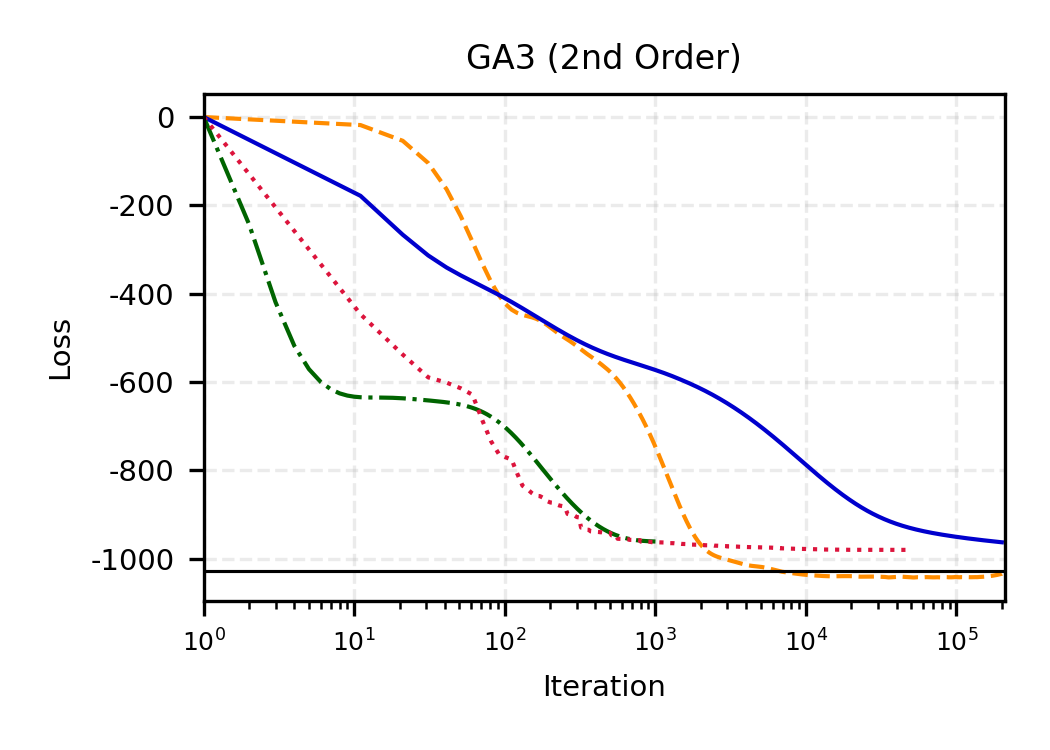
\includegraphics[width=.49\textwidth]{resources/optimization_algorithms/per_iter/TruncatedGMMAsymmetricThree_order_2_loss_per_iter.png}
    \hfill
    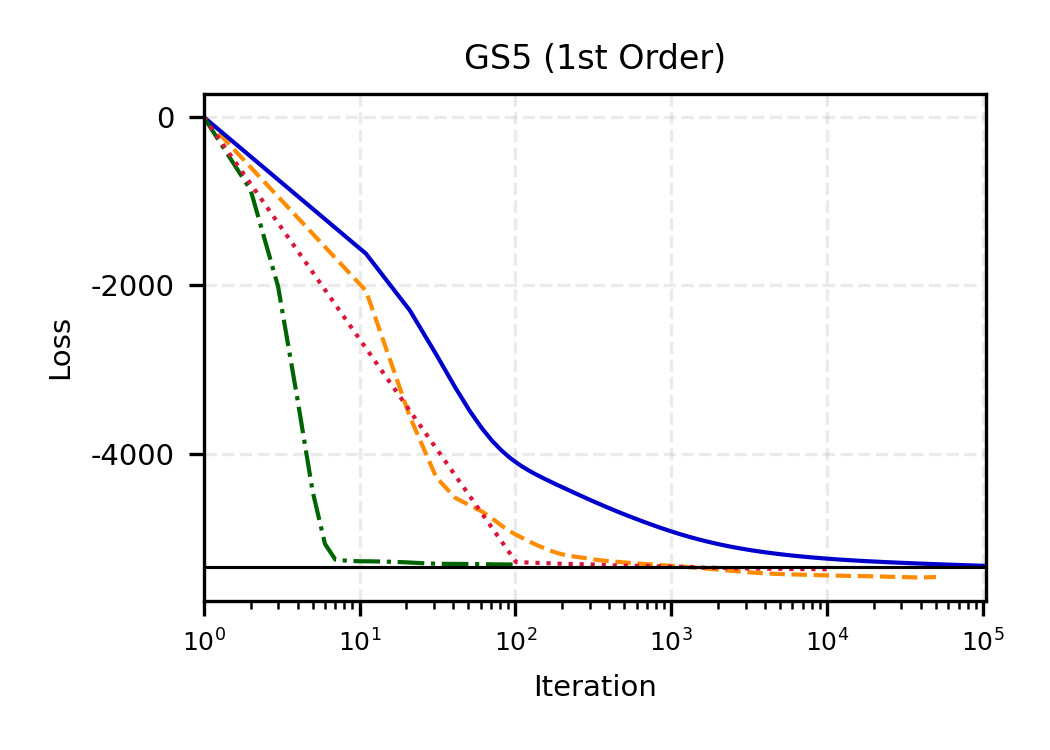
\includegraphics[width=.49\textwidth]{resources/optimization_algorithms/per_iter/TruncatedGMMFiveSpikes_order_1_loss_per_iter.png}
    
    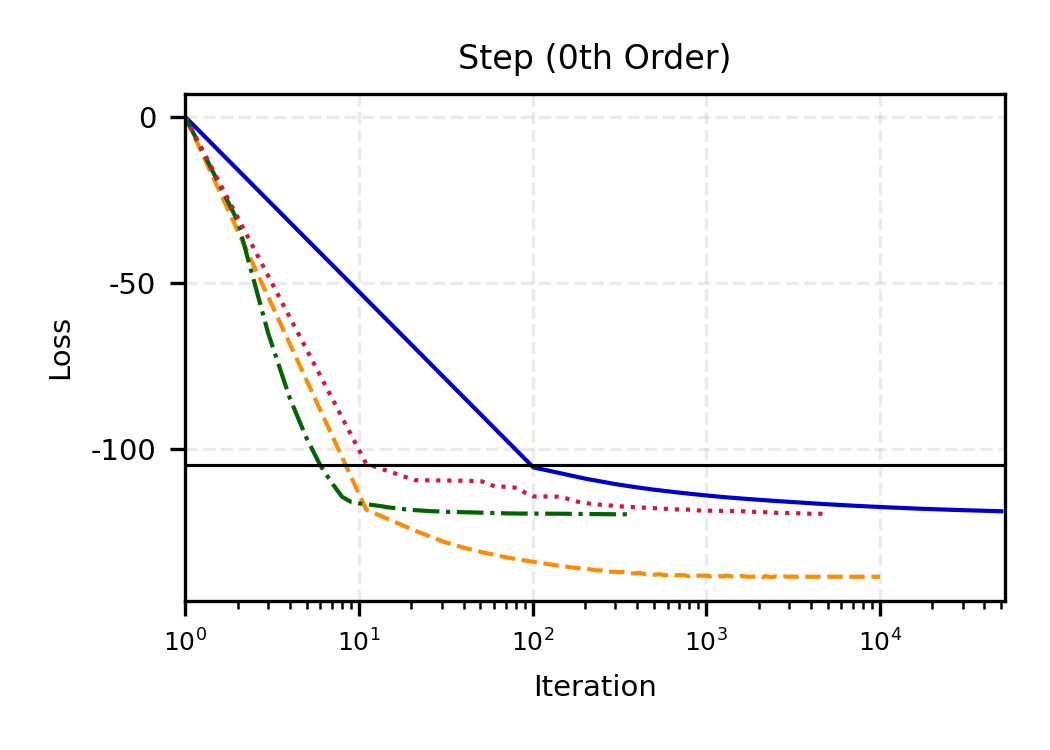
\includegraphics[width=.49\textwidth]{resources/optimization_algorithms/per_iter/StepFunction_order_0_loss_per_iter.png}
    \hfill
    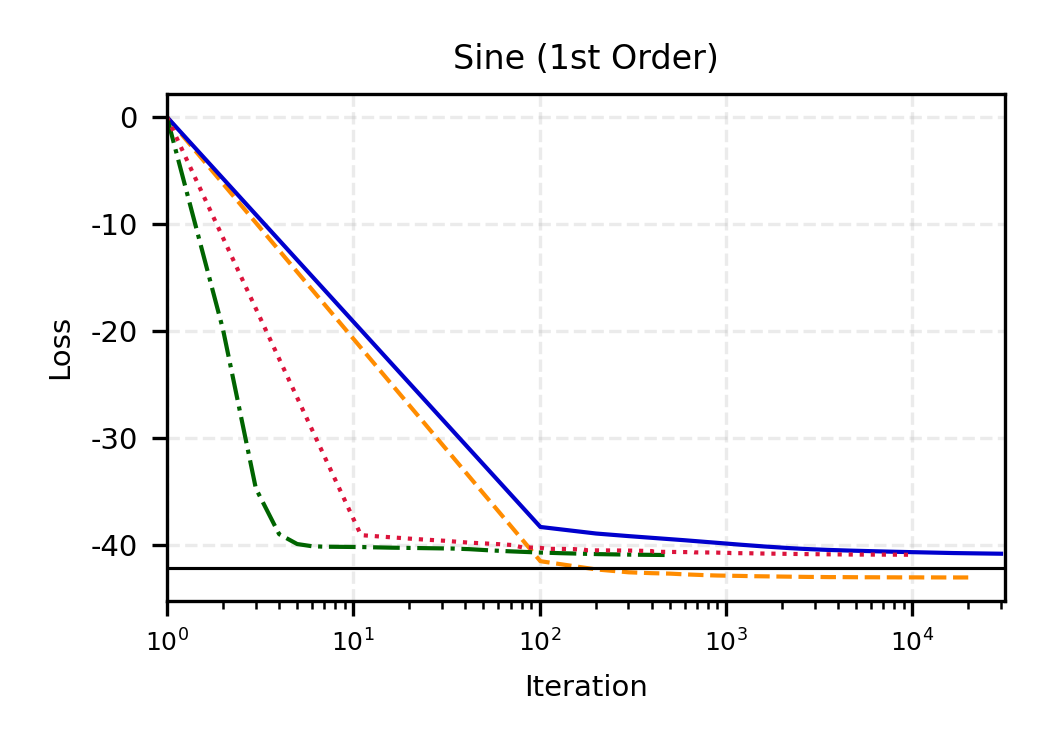
\includegraphics[width=.49\textwidth]{resources/optimization_algorithms/per_iter/Sinusoidal_order_1_loss_per_iter.png}
    
    \caption{Per-iteration loss convergence for optimization algorithms across six DGPs. Panels (row-wise, left to right): (a) TN, (b) GS3, (c) GA3, (d) GS5, (e) Step, (f) Sine.}
    \label{fig:opt-per-iter-loss}
    \end{figure}
    
    \begin{figure}[H]
    \centering
    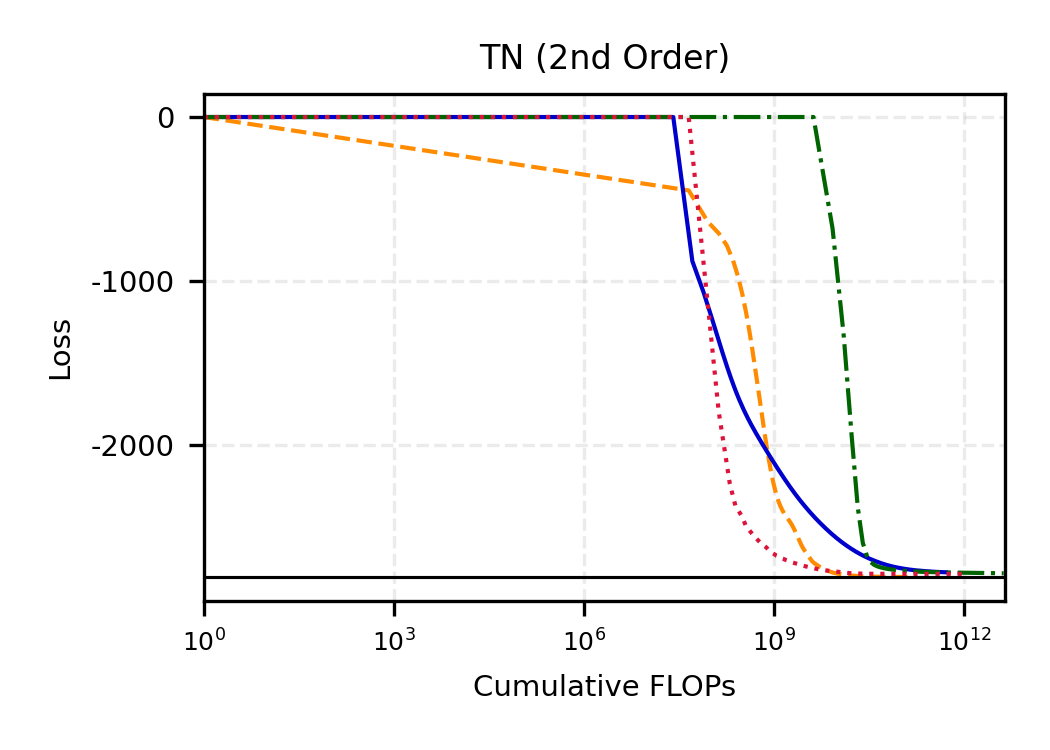
\includegraphics[width=.49\textwidth]{resources/optimization_algorithms/per_flop/TruncatedNormal_order_2_loss_per_flop.png}
    \hfill
    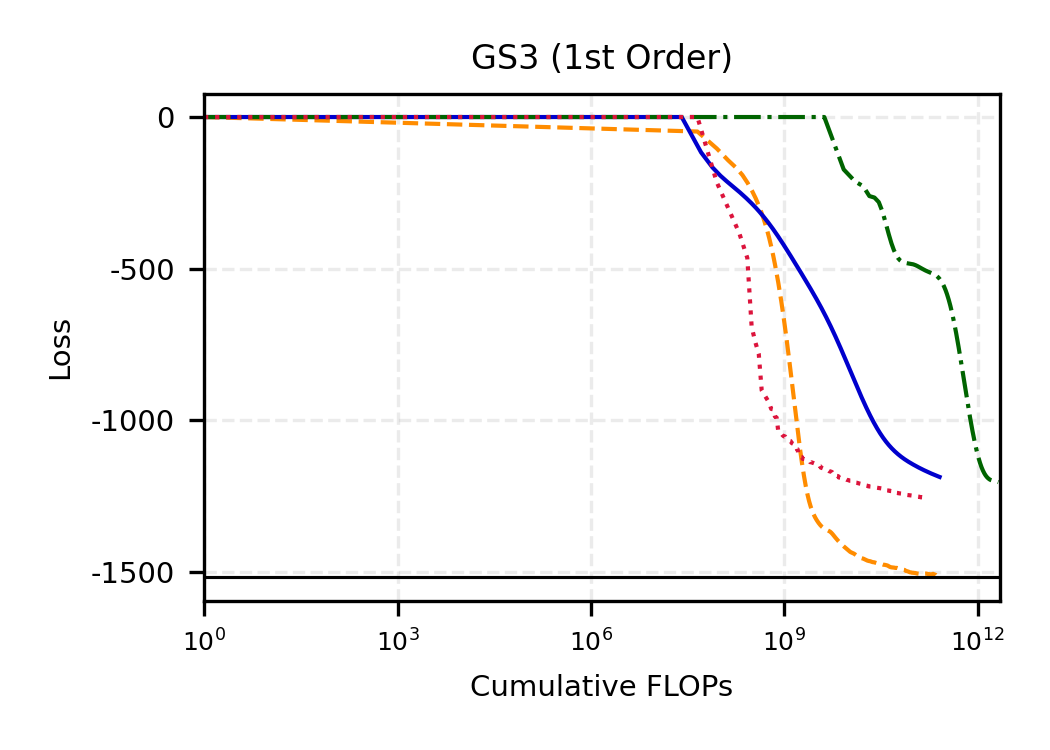
\includegraphics[width=.49\textwidth]{resources/optimization_algorithms/per_flop/TruncatedGMMSymmetricThree_order_1_loss_per_flop.png}
    
    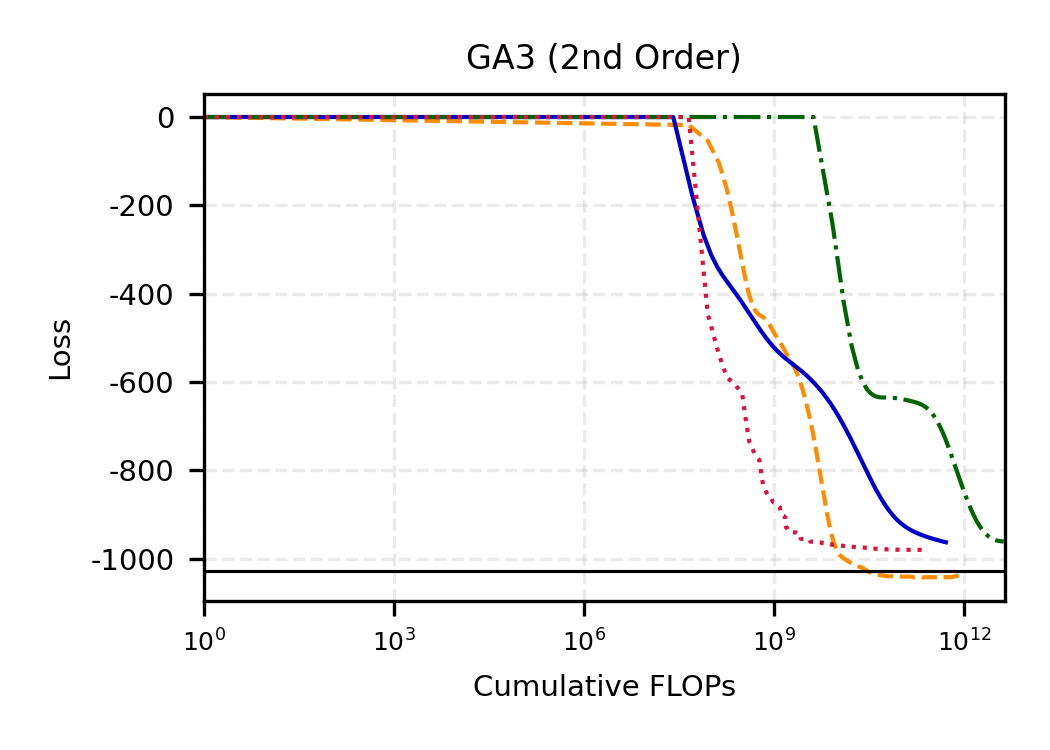
\includegraphics[width=.49\textwidth]{resources/optimization_algorithms/per_flop/TruncatedGMMAsymmetricThree_order_2_loss_per_flop.png}
    \hfill
    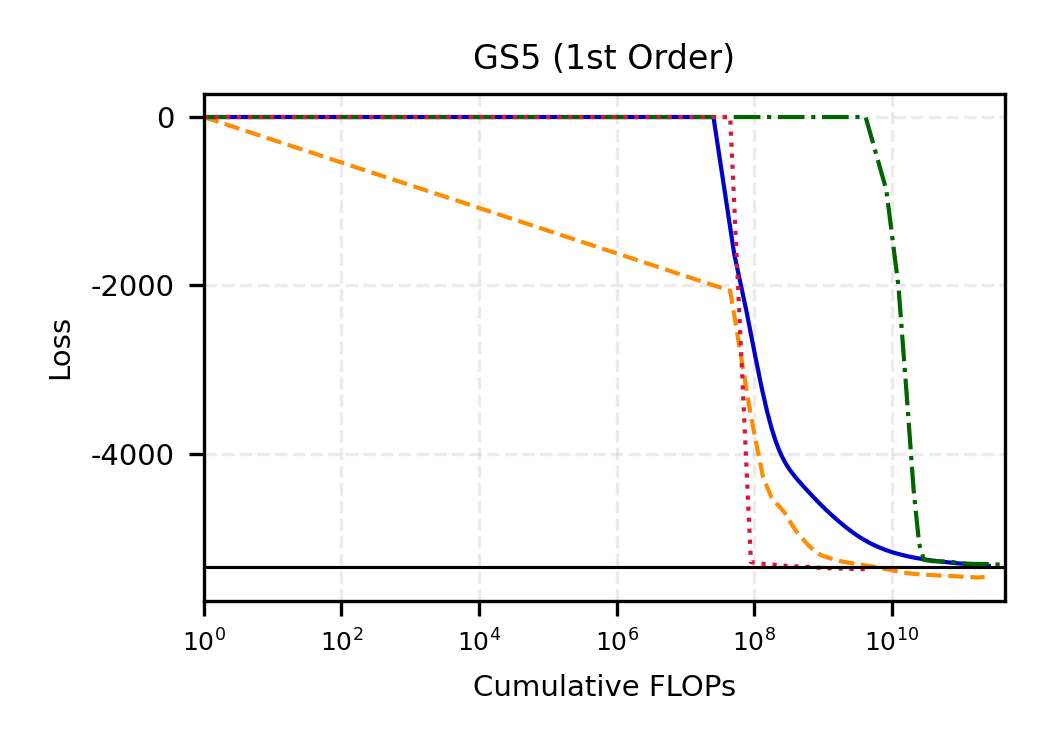
\includegraphics[width=.49\textwidth]{resources/optimization_algorithms/per_flop/TruncatedGMMFiveSpikes_order_1_loss_per_flop.png}
    
    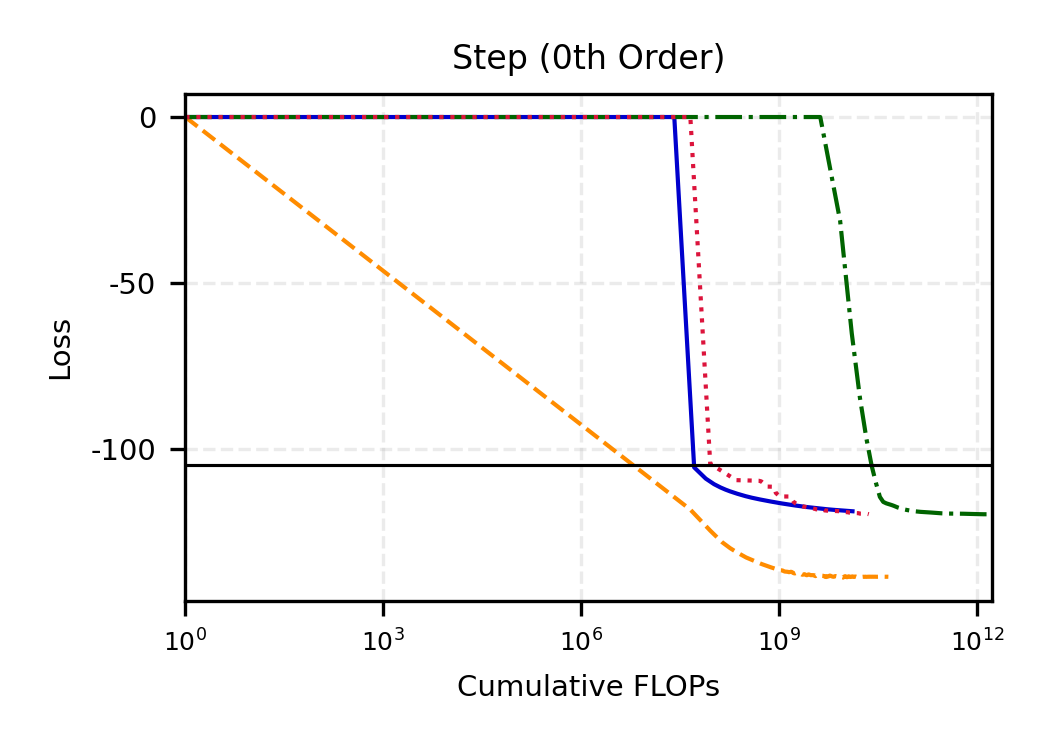
\includegraphics[width=.49\textwidth]{resources/optimization_algorithms/per_flop/StepFunction_order_0_loss_per_flop.png}
    \hfill
    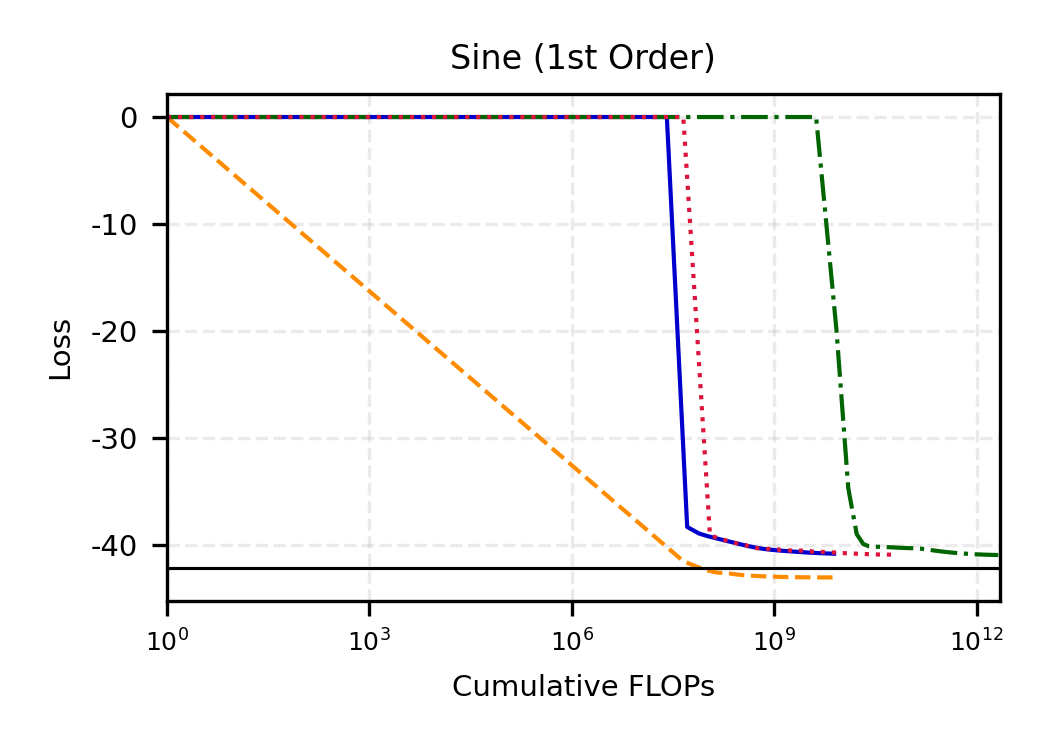
\includegraphics[width=.49\textwidth]{resources/optimization_algorithms/per_flop/Sinusoidal_order_1_loss_per_flop.png}
    
    \caption{Per-FLOP-normalized loss convergence across six DGPs. Panels (row-wise, left to right): (a) TN, (b) GS3, (c) GA3, (d) GS5, (e) Step, (f) Sine.}
    \label{fig:opt-per-flop-loss}
 \end{figure}
 
 \begin{figure}[H]
 \centering
 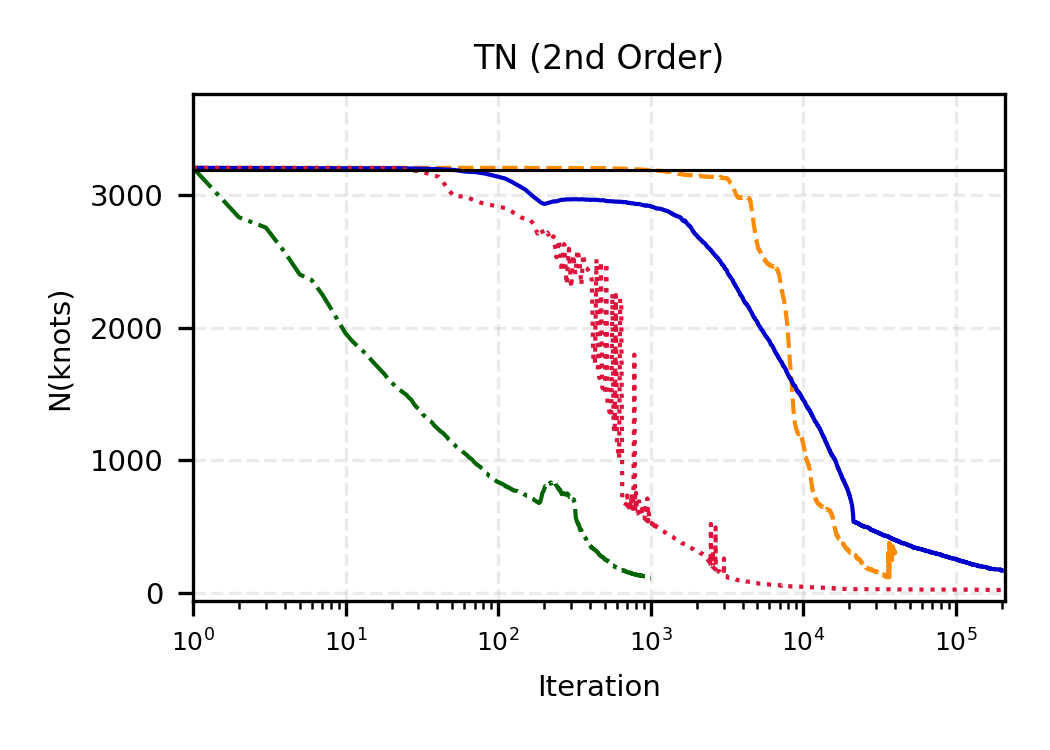
\includegraphics[width=.49\textwidth]{resources/optimization_algorithms/per_iter/TruncatedNormal_order_2_knot_selection.png}
 \hfill
 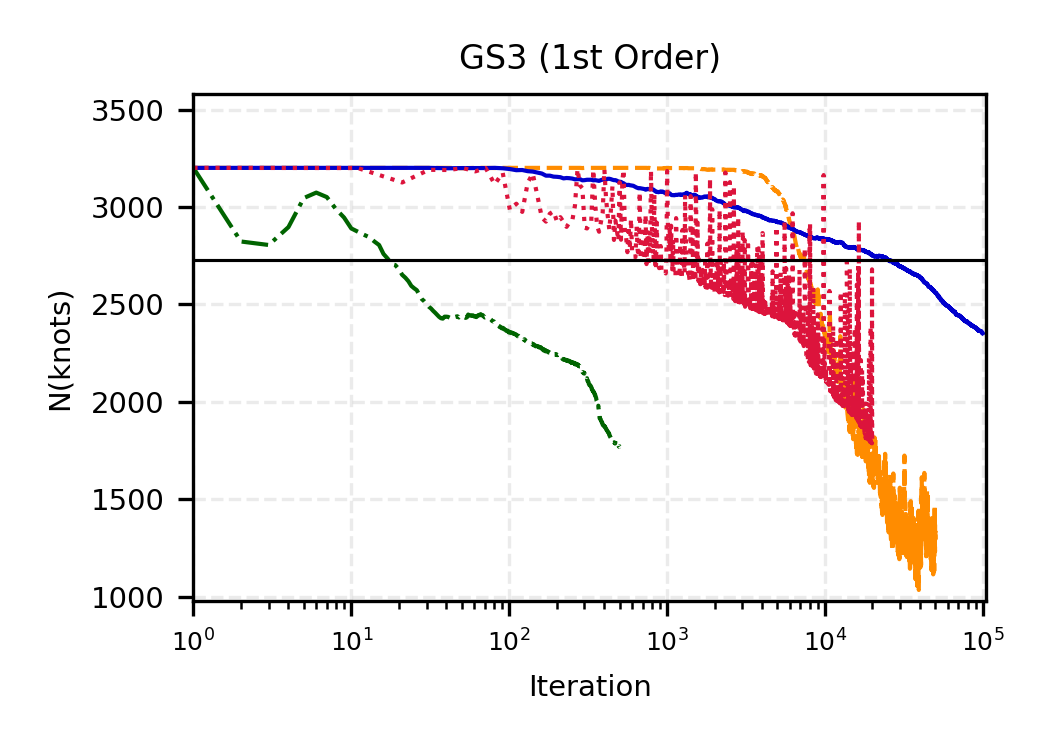
\includegraphics[width=.49\textwidth]{resources/optimization_algorithms/per_iter/TruncatedGMMSymmetricThree_order_1_knot_selection.png}
 
 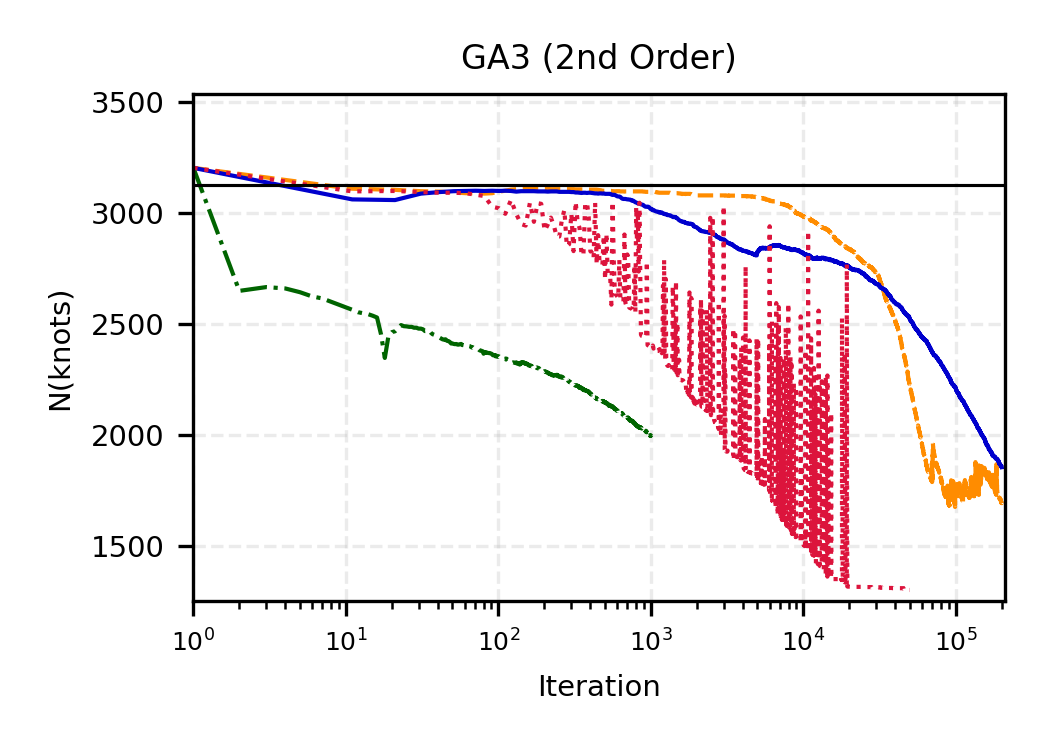
\includegraphics[width=.49\textwidth]{resources/optimization_algorithms/per_iter/TruncatedGMMAsymmetricThree_order_2_knot_selection.png}
 \hfill
 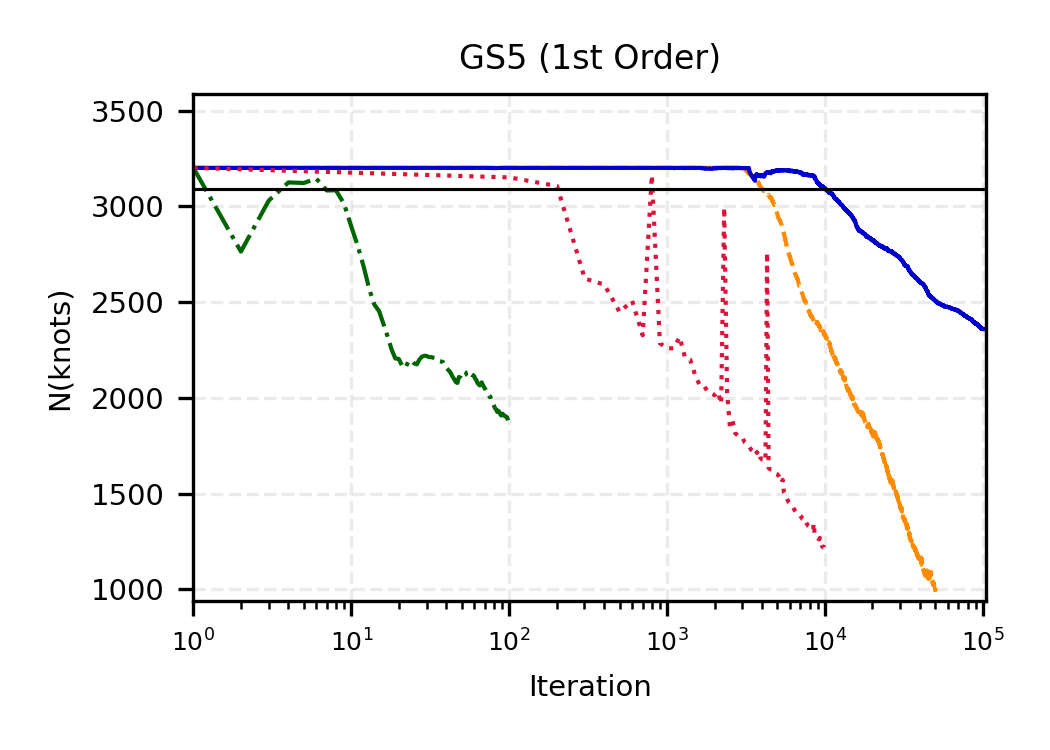
\includegraphics[width=.49\textwidth]{resources/optimization_algorithms/per_iter/TruncatedGMMFiveSpikes_order_1_knot_selection.png}
 
 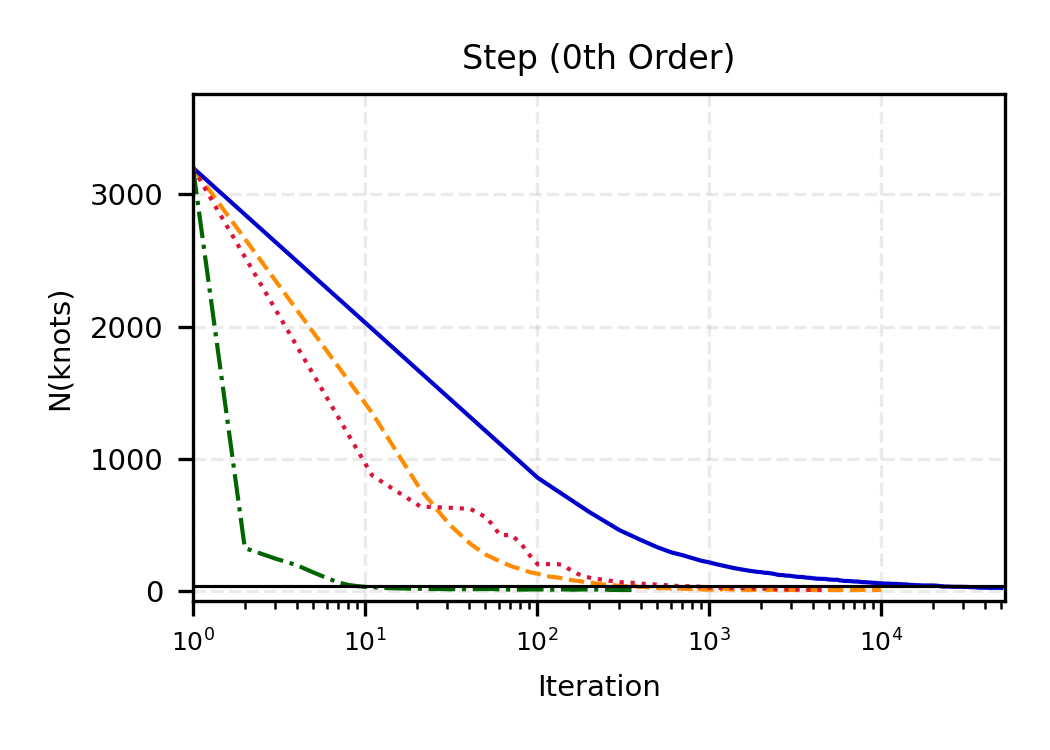
\includegraphics[width=.49\textwidth]{resources/optimization_algorithms/per_iter/StepFunction_order_0_knot_selection.png}
 \hfill
 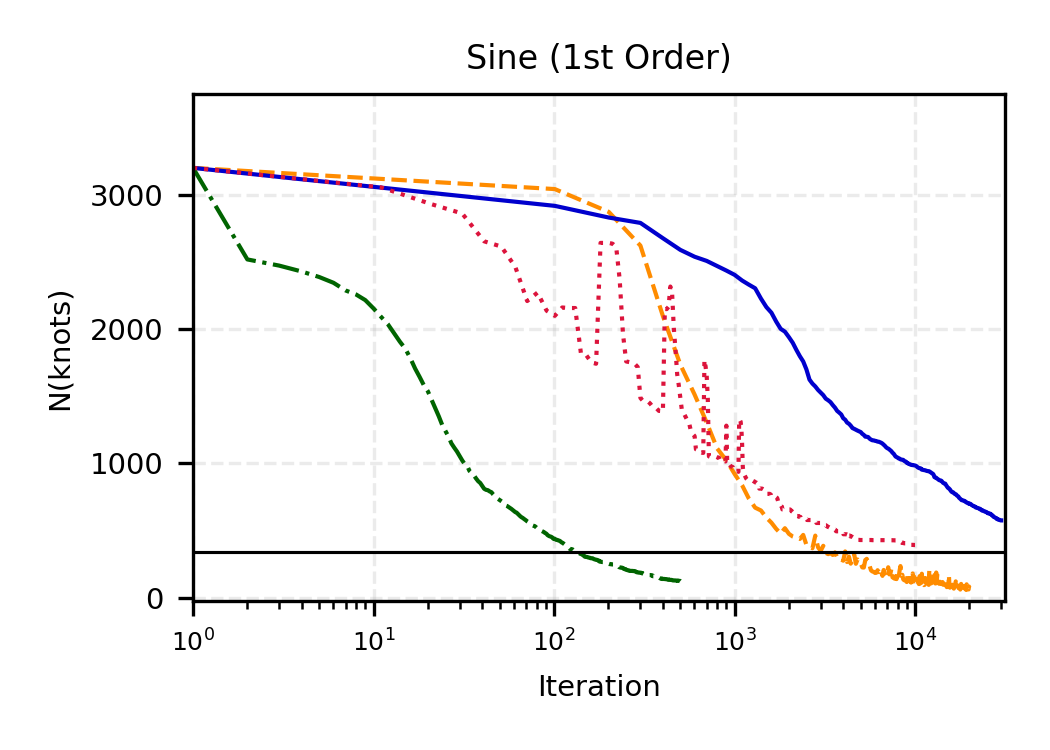
\includegraphics[width=.49\textwidth]{resources/optimization_algorithms/per_iter/Sinusoidal_order_1_knot_selection.png}
 
 \end{figure}
 
 \begin{figure}[H]
    \centering
    
\includegraphics[width=.9\textwidth]{resources/optimization_algorithms/per_iter/legend_knot_selection_algorithms.png}
    \caption{Per-iteration knot selection for optimization algorithms across six DGPs. Panels (row-wise, left to right): (a) TN, (b) GS3, (c) GA3, (d) GS5, (e) Step, (f) Sine.}
 \label{fig:opt-per-iter-knot}
 \end{figure}
 
 \begin{figure}[H]
 \centering
 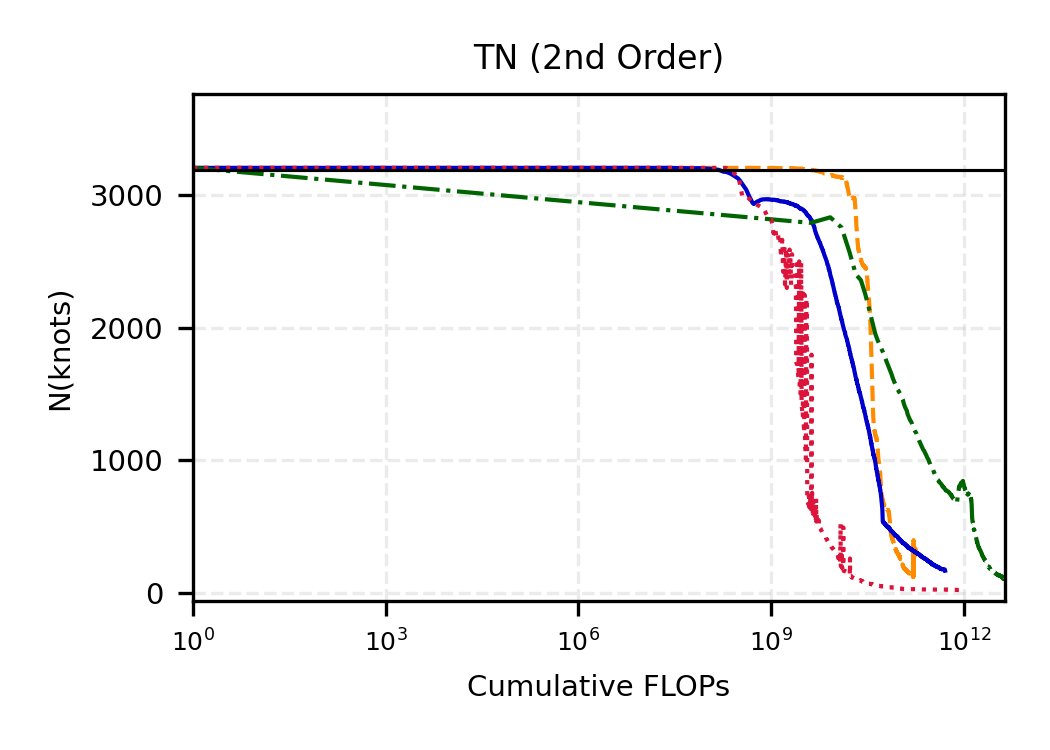
\includegraphics[width=.49\textwidth]{resources/optimization_algorithms/per_flop/TruncatedNormal_order_2_knot_selection_flops.png}
 \hfill
 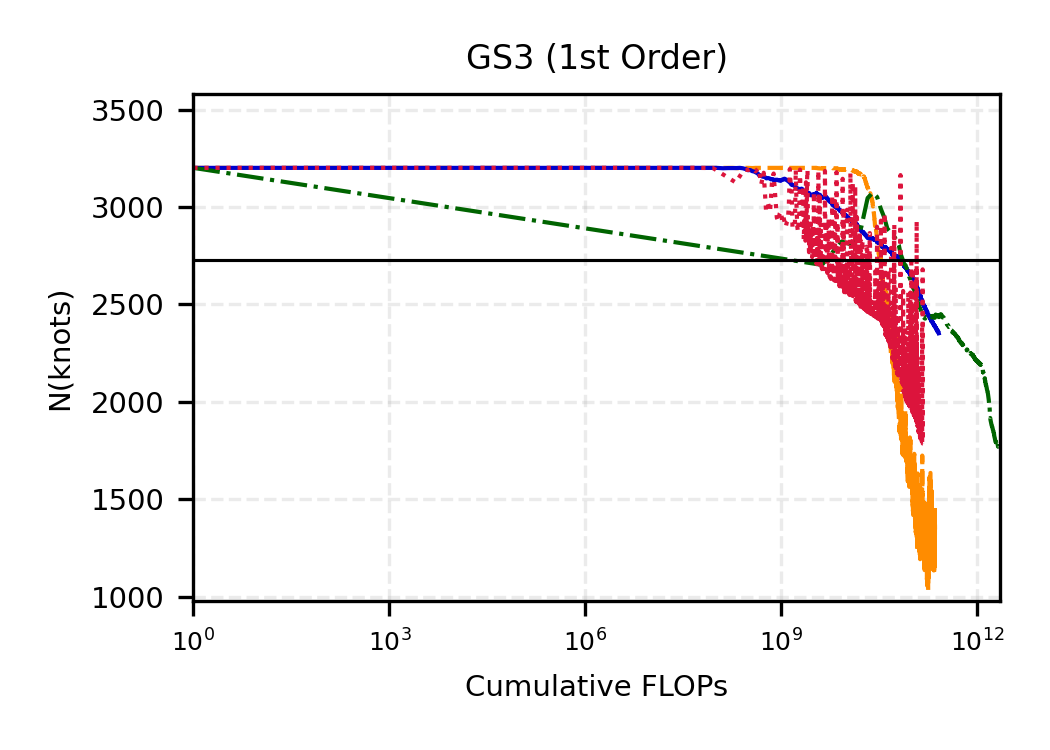
\includegraphics[width=.49\textwidth]{resources/optimization_algorithms/per_flop/TruncatedGMMSymmetricThree_order_1_knot_selection_flops.png}
 
 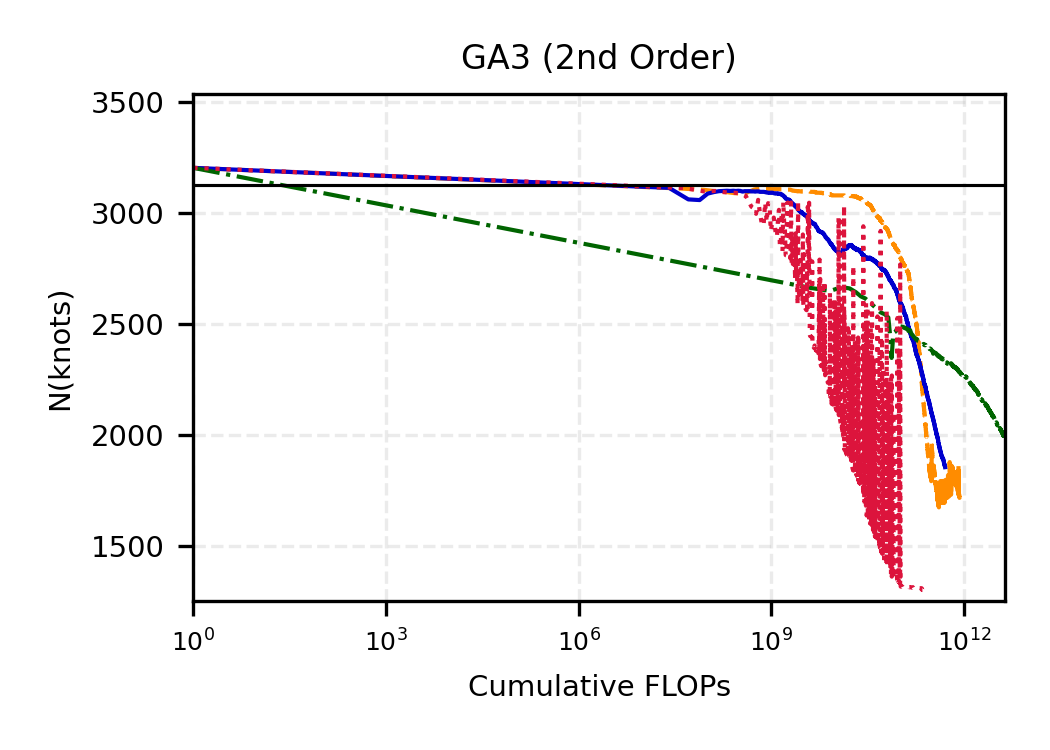
\includegraphics[width=.49\textwidth]{resources/optimization_algorithms/per_flop/TruncatedGMMAsymmetricThree_order_2_knot_selection_flops.png}
 \hfill
 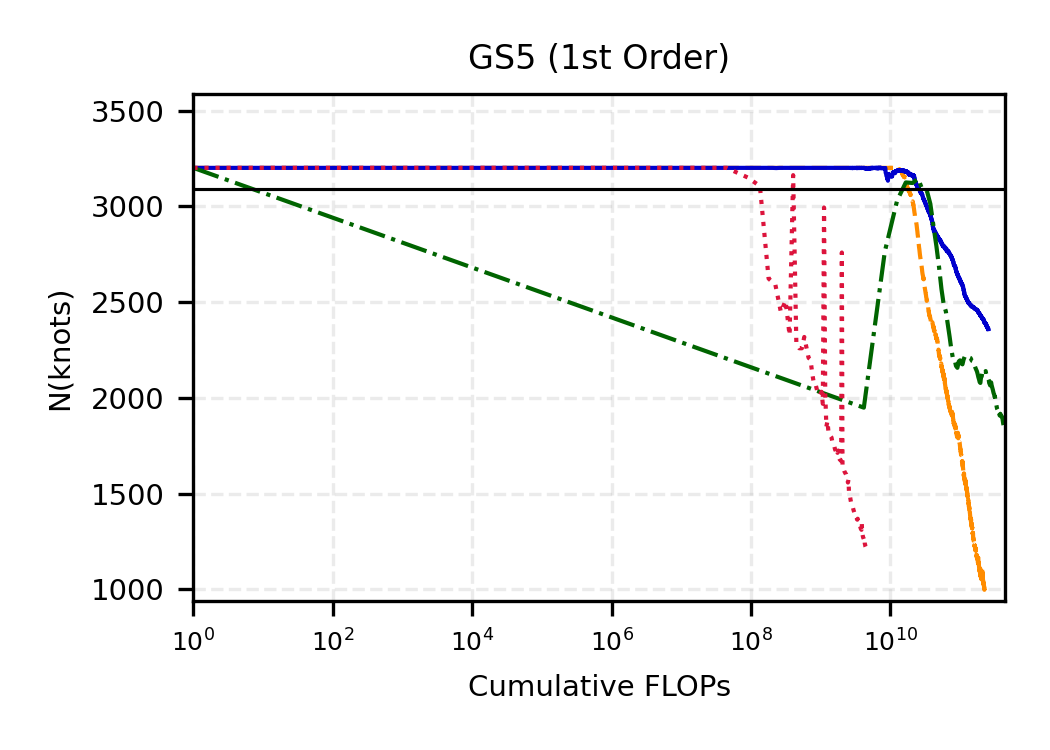
\includegraphics[width=.49\textwidth]{resources/optimization_algorithms/per_flop/TruncatedGMMFiveSpikes_order_1_knot_selection_flops.png}
 
 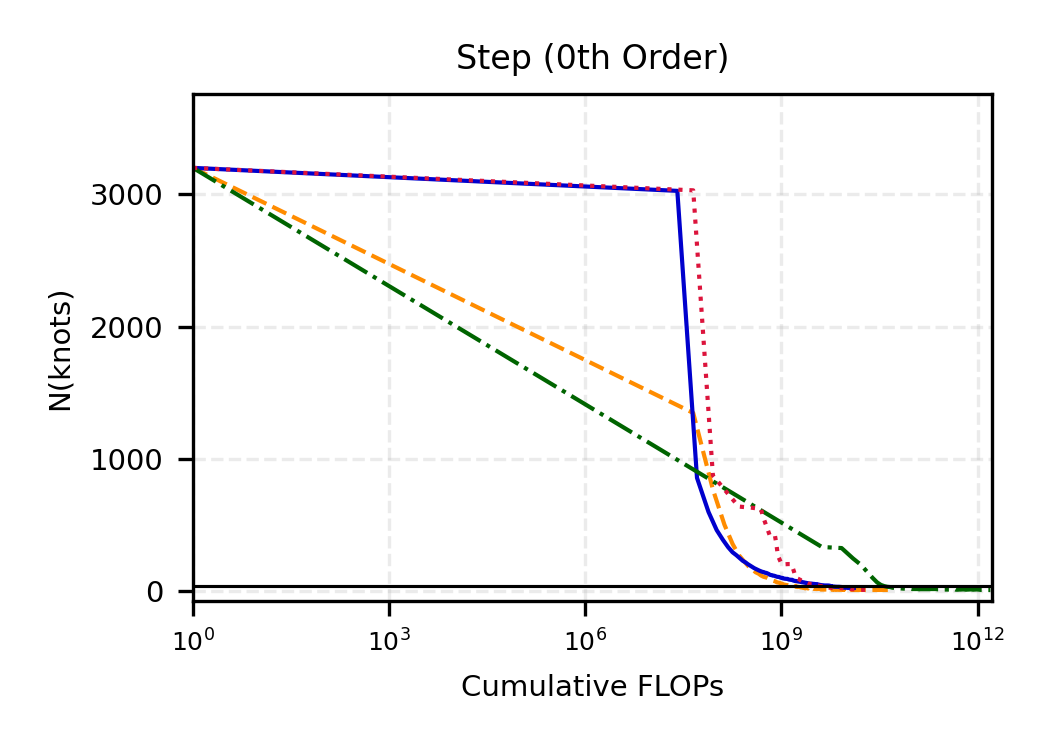
\includegraphics[width=.49\textwidth]{resources/optimization_algorithms/per_flop/StepFunction_order_0_knot_selection_flops.png}
 \hfill
 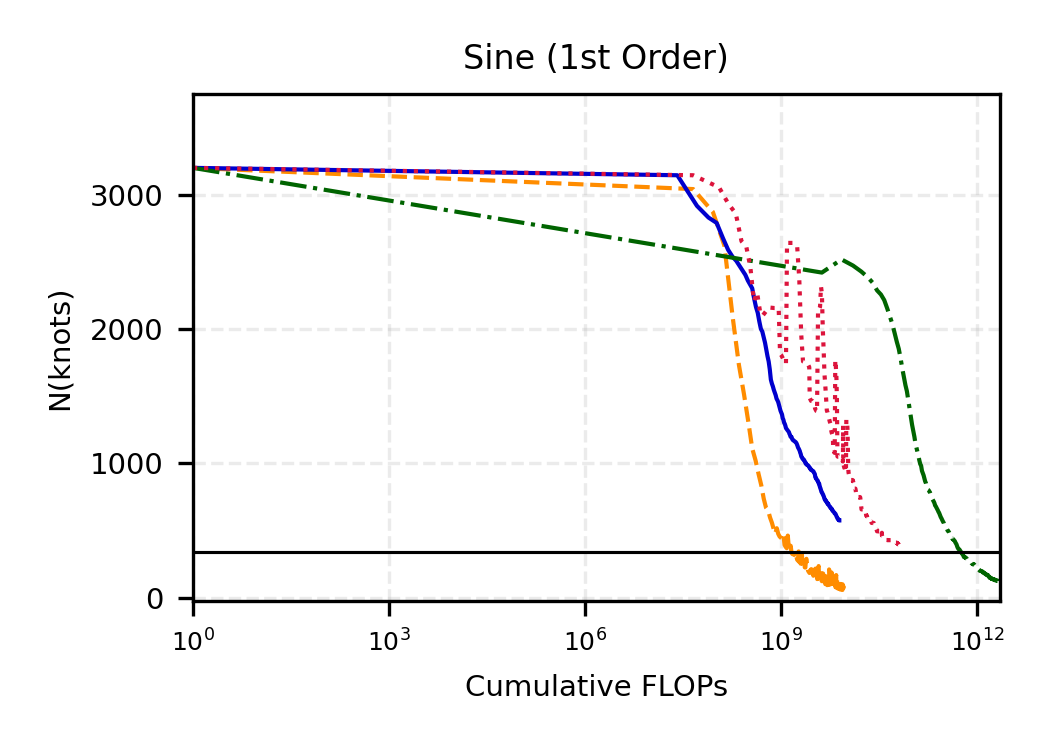
\includegraphics[width=.49\textwidth]{resources/optimization_algorithms/per_flop/Sinusoidal_order_1_knot_selection_flops.png}
 \end{figure}
 
 \begin{figure}[H]
    \centering
    
\includegraphics[width=.9\textwidth]{resources/optimization_algorithms/per_iter/legend_knot_selection_algorithms.png}
    \caption{Per-FLOP-normalized knot selection across six DGPs. Panels (row-wise, left to right): (a) TN, (b) GS3, (c) GA3, (d) GS5, (e) Step, (f) Sine.}
    \label{fig:opt-per-flop-knot}
 \end{figure}
 

\bibliographystyle{imsart-nameyear}
\bibliography{ref}

\end{document}
